%%%%%%%%%%%%%%%%%%%%%%%%%%%%%%%%%%%%%%%%%
% kaobook
% LaTeX Template
% Version 1.0 (5/6/19)
%
% This template originates from:
% https://www.LaTeXTemplates.com
%
% For the latest template development version and to make contributions:
% https://github.com/fmarotta/kaobook
%
% Authors:
% Federico Marotta (federicomarotta@mail.com)
% Based on the doctoral thesis of Ken Arroyo Ohori (https://3d.bk.tudelft.nl/ken/en)
% and on the Tufte-LaTeX class.
% Modified for LaTeX Templates by Vel (vel@latextemplates.com)
%
% License:
% CC0 1.0 Universal (see included MANIFEST.md file)
%
%%%%%%%%%%%%%%%%%%%%%%%%%%%%%%%%%%%%%%%%%

%----------------------------------------------------------------------------------------
%	PACKAGES AND OTHER DOCUMENT CONFIGURATIONS
%----------------------------------------------------------------------------------------

\documentclass[
	fontsize=12pt, % Base font size
	twoside=true, % Use different layouts for even and odd pages (in particular, if twoside=true, the margin column will be always on the outside)
	%open=any, % If twoside=true, uncomment this to force new chapters to start on any page, not only on right (odd) pages
	%chapterprefix=true, % Uncomment to use the word "Chapter" before chapter numbers everywhere they appear
	%chapterentrydots=true, % Uncomment to output dots from the chapter name to the page number in the table of contents
	numbers=noenddot, % Comment to output dots after chapter numbers; the most common values for this option are: enddot, noenddot and auto (see the KOMAScript documentation for an in-depth explanation)
	%draft=true, % If uncommented, rulers will be added in the header and footer
	%overfullrule=true, % If uncommented, overly long lines will be marked by a black box; useful for correcting spacing problems
]{kaobook}

% Choose the language
\usepackage[english]{babel} % Load characters and hyphenation
\usepackage[english=british]{csquotes}	% English quotes
\usepackage{dsfont}

% Load packages for testing
\usepackage{blindtext}
%\usepackage{showframe} % Uncomment to show boxes around the text area, margin, header and footer
%\usepackage{showlabels} % Uncomment to output the content of \label commands to the document where they are used

% Load the bibliography package
\usepackage{styles/kaobiblio}
%\addbibresource{main.bib} % Bibliography file
\addbibresource{bibliographies/styletransfer.bib} % Bibliography file
\addbibresource{bibliographies/brushstrokes.bib} % Bibliography file
\addbibresource{bibliographies/painters.bib} % Bibliography file

% Load mathematical packages for theorems and related environments. NOTE: choose only one between 'mdftheorems' and 'plaintheorems'.
\usepackage{styles/mdftheorems}
%\usepackage{styles/plaintheorems}

\graphicspath{{examples/documentation/images/}{images/}} % Paths in which to look for images

\makeindex[columns=3, title=Alphabetical Index, intoc] % Make LaTeX produce the files required to compile the index

% Reset sidenote counter at chapters
%\counterwithin*{sidenote}{chapter}
\DeclareMathAlphabet{\mathcal}{OMS}{cmsy}{m}{n}

\newcommand\norm[1]{\left\lVert#1\right\rVert}
%\renewcommand\vec[1]{\underline#1}
\newcommand\mat[1]{\underline{\underline{#1}}}
\newcommand\tensor[1]{\mathbf{#1}}
\newcommand\R{\mathbb{R}}
\newcommand\E{\mathbb{E}}
\renewcommand\L{\mathcal{L}}

\usepackage{amsmath}
\usepackage[binary-units=true]{siunitx}
\DeclareMathOperator*{\argmax}{arg\,max}
\DeclareMathOperator*{\argmin}{arg\,min}
%----------------------------------------------------------------------------------------

\usepackage{import}
\subimport{./images/PlotNeuralNet/layers/}{init}
\usetikzlibrary{positioning}

\def\ConvColor{rgb:yellow,5;red,2.5;white,5}
\def\ConvReluColor{rgb:yellow,5;red,5;white,5}
\def\PoolColor{rgb:red,1;black,0.3}
\def\FcColor{rgb:blue,5;red,2.5;white,5}
\def\FcReluColor{rgb:blue,5;red,5;white,4}
\def\SoftmaxColor{rgb:magenta,5;black,7}

\usepackage{pgfplots}

%\spacing{1.5}
\onehalfspacing

\usepackage{styles/dictionary}
\dictshorthand{CAD}{Cambridge American Dictionary}
\dictshorthand{MW}{Merriam-Webster}
\dictlibrary{mylib}

\usepackage{subfig}

\usepackage{xpatch}

\xpatchbibmacro{name:andothers}{%
  \bibstring{andothers}%
}{%
  \bibstring[\textit]{andothers}%
}{}{}

\usepackage{listings}
\definecolor{darkblue}{HTML}{000099}
%\def ¡{|}

\lstset{
    frameround=fttt,
    language=C,
    numbers=left,
    %stepnumber=5,               % Abstand zwischen den Zeilennummern       
    %numberfirstline=false
    breaklines=true,
    keywordstyle=\color{black}\bfseries, 
    basicstyle=\ttfamily\footnotesize\color{darkblue},
    showstringspaces=false,
    numberstyle=\color{black}
    }

\begin{document}

%----------------------------------------------------------------------------------------
%	BOOK INFORMATION
%----------------------------------------------------------------------------------------

\titlehead{Universität Heidelberg}
\subject{Fakultät für Physik}

\title[Artificially Painting]{Artificially Painting Pictures \& Artworks}
\subtitle{Masters Thesis}

\author[Arthur Willy Heimbrecht]{Arthur Willy Heimbrecht}

\date{June 2nd 2020}

\publishers{supervised by Professors Björn Ommer and Tilman Plehn}

%----------------------------------------------------------------------------------------

\frontmatter % Denotes the start of the pre-document content, uses roman numerals

%---------------------------------------------------------------------------------------
%        OPENING PAGE & Abstract
%----------------------------------------------------------------------------------------

\makeatletter
\extratitle{
	% In the title page, the title is vspaced by 9.5\baselineskip
	\vspace*{9\baselineskip}
	\vspace*{\parskip}
	\begin{center}
		% In the title page, \huge is set after the komafont for title
		\usekomafont{title}\huge\@title
	\end{center}
}
\makeatother

%----------------------------------------------------------------------------------------
%	OUTPUT TITLE PAGE AND PREVIOUS
%----------------------------------------------------------------------------------------

% Note that \maketitle outputs the pages before here

% If twoside=false, \uppertitleback and \lowertitleback are not printed
% To overcome this issue, we set twoside=semi just before printing the title pages, and set it back to false just after the title pages
\KOMAoptions{twoside=semi}
\maketitle
\KOMAoptions{twoside=false}

%----------------------------------------------------------------------------------------
%	PREFACE
%----------------------------------------------------------------------------------------

\chapter*{Preface}
\addcontentsline{toc}{chapter}{Preface} % Add the preface to the table of contents as a chapter

I am of the opinion that every \LaTeX\xspace geek, at least once during 
his life, feels the need to create his or her own class: this is what 
happened to me and here is the result, which, however, should be seen as 
a work still in progress. Actually, this class is not completely 
original, but it is a blend of all the best ideas that I have found in a 
number of guides, tutorials, blogs and tex.stackexchange.com posts. In 
particular, the main ideas come from two sources:

\begin{itemize}
	\item \href{https://3d.bk.tudelft.nl/ken/en/}{Ken Arroyo Ohori}'s 
	\href{https://3d.bk.tudelft.nl/ken/en/nl/ken/en/2016/04/17/a-1.5-column-layout-in-latex.html}{Doctoral 
	Thesis}, which served, with the author's permission, as a backbone 
	for the implementation of this class;
	\item The 
		\href{https://github.com/Tufte-LaTeX/tufte-latex}{Tufte-Latex 
			Class}, which was a model for the style.
\end{itemize}

The first chapter of this book is introductive and covers the most 
essential features of the class. Next, there is a bunch of chapters 
devoted to all the commands and environments that you may use in writing 
a book; in particular, it will be explained how to add notes, figures 
and tables, and references. The second part deals with the page layout 
and design, as well as additional features like coloured boxes and 
theorem environments.

I started writing this class as an experiment, and as such it should be 
regarded. Since it has always been indended for my personal use, it may 
not be perfect but I find it quite satisfactory for the use I want to 
make of it. I share this work in the hope that someone might find here 
the inspiration for writing his or her own class.

\begin{flushright}
	\textit{Federico Marotta}
\end{flushright}


%----------------------------------------------------------------------------------------
%	TABLE OF CONTENTS & LIST OF FIGURES/TABLES
%----------------------------------------------------------------------------------------

\begingroup % Local scope for the following commands

% Define the style for the TOC, LOF, and LOT
%\setstretch{1} % Uncomment to modify line spacing in the ToC
%\hypersetup{linkcolor=blue} % Uncomment to set the colour of links in the ToC
\setlength{\textheight}{23cm} % Manually adjust the height of the ToC pages

% Turn on compatibility mode for the etoc package
\etocstandarddisplaystyle % "toc display" as if etoc was not loaded
\etocstandardlines % "toc lines as if etoc was not loaded

\tableofcontents % Output the table of contents

\endgroup

%----------------------------------------------------------------------------------------
%	MAIN BODY
%----------------------------------------------------------------------------------------

\mainmatter % Denotes the start of the main document content, resets page numbering and uses arabic numbers
\setchapterstyle{kao} % Choose the default chapter heading style

%\input{chapters/Introduction.tex}
%
%\pagelayout{wide} % No margins
%\addpart{Theoretical Background \& Related Work}
%\pagelayout{margin} % Restore margins
%
%\setchapterpreamble[u]{\margintoc}
\chapter{Machine Learning \& Computer Vision}
\labch{MLandCV}
In this chapter the theoretical backgrounds and motivation of Neural Networks ought to be explored.

First, a physical/biological motivation will set the foundation for the theoretical background accompanied by a more mathematical motivation.
Thereafter, more advanced lines of thought will be introduced that finally lead to convolutional neural networks as the current driving force in computer vision .

\section[Artificial NNs]{Artificial Neural Networks}

\subsection[Inspiration]{Neurobiological Inspiration}

%Nature is often inspiration (birds and planes)
Many human achievements have at least been partially inspired by studying nature.
A very popular example is that of airplanes and birds.
The study of how birds are able to fly found that the shape of their wing is the essential element to flying.
Inventors and engineers have taken this inspiration and slowly but steadily created planes and the like from it.
%arguabnly implementations deviate from nature (plane and bird) and people say to refrain from using these analogies.
Yet, planes are not birds, as they are not flapping their wings (yet?), but integrate of other inventions like jet engines to get the same (or better) capability of flying as birds.

Quite similarly, the brain features a lot of insights, how intelligence or something that seems like it, can be constructed.
In the same way humans studied birds to understand flying, researchers are now studying the brain to create better artificial intelligence.

In the earliest stages of this they would try to imitate the brain, as people have tried imitating birds at first and failed similarly.
\begin{figure}
    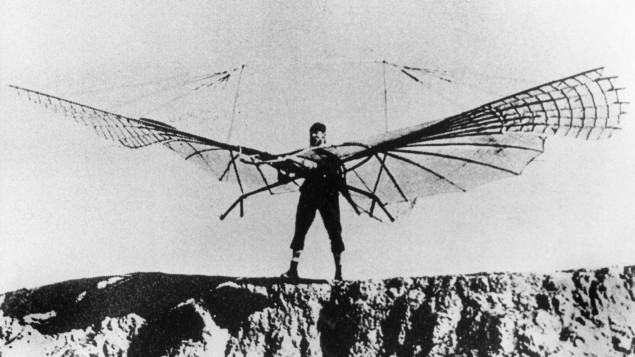
\includegraphics{otto_lilienthal}
    \caption[]{Otto Lilienthal with his flying apparatus. \url{https://www.deutschlandfunkkultur.de/geschichte-der-fliegerei-wie-der-mensch-die-voegel.976.de.html?dram:article_id=308043}}
    \labfig{lilienthal}
\end{figure}
\marginnote{There is current research on replicating the brains structure to the neuron level on hardware with more success \cite{brainscales}.}

%start with a very much simplified model McCulloch and Pitts
%binary input and binary output
Warren McCulloch and Walter Pitts proposed one of the earliest models of a neuron, which targeted simplifying the real Neuron.
\marginnote{Notably McCulloch and Pitts (1943) even preceded Hodkins and Huxley's (1952) Nobel price winning description of a neuron.}

%explain biological neuron
\subsubsection{Biological Neuron}
For this the functioning of a neuron shall be described shortly.

Human cells in that make up the brain are called \textbf{neurons}.
They connected to each other through dendrites, synapses and axons and they use these connections to send signals.

A neuron receives signals through its dendrites, which all lead to the cell body (soma).
At the cell body the signals are accumulated.
If the summed value of the signals' potential reaches a certain threshold, an action potential is generated.
The new signal then travels along the axon and its branches towards other neurons.
The axon ends in synapses which connect the axon to other neurons' dendrites.
Synaptic transmissions are usually mediated by chemicals and not by electrical signals.
The chemical nature of the synapse allows it to forward either an excitatory or an inhibitory signal.
Excitatory signals will bring the cell potential closer to the threshold, while inhibitory do the opposite \cite[p.~42]{coloratlas}.
\marginnote{Cell potentials are usually decreases by excitatory signals, as the action threshold sits below the resting potential.}

What makes the brain so powerful though, is not the neuron itself with its arguably simple structure but the vast network of billions of these neurons.
Each neuron is connected to thousands of other neurons with which it constantly communicates.
How a signal is transported between the neurons depends on the interplay of synaptic weights, neuron connections and the threshold of each neurons.

\subsubsection{Artificial Neuron}
McCulloch and Pitts saw that powerful things can be achieved when connecting lots and lots of simple structures.
Thus, they proposed an even simpler model of a neuron:

They restricted their neuron to a binary state (on or off).
Each neuron then has a number of incoming signals from other neurons which would either be positive or negative.
A neuron would only become active if the number of incoming positive signals minus the number of negative signals exceeds the neuron's threshold.
\todo{add equation with activation function, when neuron fires}
McCulloch and Pitts then also changed the highly parallel and complex nature of biological neural networks to a single layer feed-forward network architecture.

In a feed-forward network neurons are grouped into layers and operate in parallel within a layer.
Each neuron in a layer is fed the same input signal (often described as an input layer).
The neuron's state is then computed according to an equation such as \refeq{mcculloch}.
The activation value of each neuron then defines an output.

As this models deviates from nature quite a bit, these structures a better referred to as \textbf{units} instead of neurons.

In a single layer architecture a layer often consists of a single unit (see \reffig{ff_arch}.
Basically, input signals come from one side and output signal go out the other side, which can be expressed in a simple equation like \refeq{mcculloch}.
This is not only done for practical reasons but also inspired by observation of layered neuron structures in the brain.

The McCulloch-Pitts model is capable of emulating simple logical relations (|AND|, |OR|, |NOT|) but nor |XOR| which will be explained later.

\subsubsection{Perceptron}
This McCulloch's and Pitts' is very much simplified yet comes with some weaknesses.
Thus, the \textbf{perceptron} has been introduced by Frank Rosenblatt in 1957.
Instead of having a binary unit, he came up with a linear threshold unit (LTU).
The LTU allows for numeric instead of binary signals which can be weighted with independent factors.
Also they use the 'bias trick' to parametrize the threshold or bias of the unit as yet another weight for an input that is constantly one.
The resulting equation for each LTU then reads:
\todo{equation for LTU with bias trick}
Equation \refeq{LTU} can then be formulated in a vectorized form such that:
\todo{vectorized LTU}

In this form the calculations for each unit become mathematically and computationally relatively easy.
Each layer can be expressed as a vector of activations $\vec{x}$.
Multiplying this vector with the weight matrix $\mat{W}$ and applying the element-wise activation function returns the activations for the subsequent layer.
\marginnote{The word perceptron describes the whole function $f$ in equation \refeq{perceptron} which can consist of many LTUs}
%simplified computational model of how biological neurons might work together
This simple yet capable description of a unit built the base for a first surge of interest in neural networks.
%connectionism

\subsubsection{Mathematical Interpretation}
%hyperplane
%linear separation
%bias trick
The very simplistic mathematical formulation of the perceptron suggests that there might be a mathematical meaning to it besides the biological analogy.
Indeed, the perceptron is equal to the definition of a \textbf{binary linear classifier}.

A binary linear classifier, classifies inputs into two classes, hence binary.
It does so by drawing a virtual hyperplane in input space and predicts the class for each input, depending on whether it lies above or below this hyperplane.
\begin{marginfigure}
    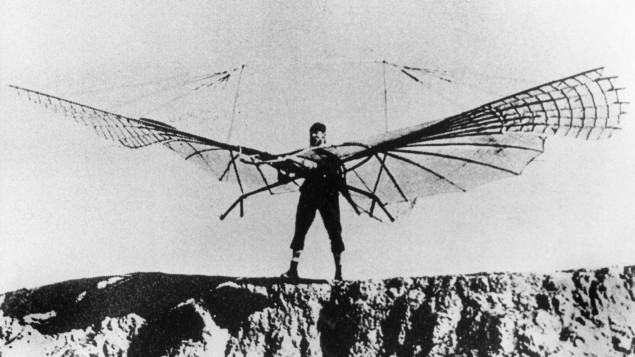
\includegraphics{otto_lilienthal}
    \caption[]{As a very simple example, this binary classifier has data on how often the words 'weightloss' and 'invest' appear in an email.
Any time these two words appears too often and the data point is above the decision boundary, the email is classified as 'spam'}
    \labfig{linear_class}
\end{marginfigure}
As the hyperplane (or decision boundary) is quantified by a linear function, the classifier is described as linear.

A classic problem would be classifying email as spam.
Given the two data inputs (\ie frequency of of the words 'weight loss' and 'invest') the classifier has to make a decision.
For this reason the binary classifier defines a \textbf{decision boundary}.
Any data point that lies above this decision boundary is classified as 'spam', any point beneath is classified as 'not spam'
This makes sense as normal email rarely use the two words.
For other people like a nutritionist, the word weight-loss can come up more frequently.
This means the decision boundary differs for different users and their mail.

To compute where a point lies relative to the decision boundary, a data point's value along each axis $x_1, x_2$ is weighted individually $w_1, w_2$ and summed with a bias $b$.
The result is checked whether it is above or below a threshold $t$.
\begin{align}
    z = w_1 x_1 + w_2 x_2 + b
\end{align}
With the classification 'spam' if $z > r$ and 'not-spam' $z \leq r$ (\textit{in dubio pro reo}).
Equally $z - r > 0$ holds for spam as well such that the threshold can be brought into the equation and $z$ is checked against $0$.
$r$ can then be absorbed into the bias.
%predistion is y, 1 is spam, 0 is not spam
\begin{align}
    \rightarrow z = w_1 x_1 + \hdots + w_D x_D + b - r = w_1 x_1 + \hdots + w_D x_D + b'
\end{align}

For arbitrary dimensions $D$ this becomes
\begin{align}
    z = w_1 x_1 + \hdots + w_D x_D + b
\end{align}
 where $\vec{x}$ and $\vec{w}$ can be defined by vectors
\begin{align}
    z = w_1 x_1 + \hdots + w_D x_D + b = \vec{w}^T \vec{x} + b
\end{align}
The decision boundary can be easily derived from this, since $\vec{w}$ is the orthogonal vector to the hyperplane and $\frac{b}/\norm{\vec{w}}$ is the displacement of the plane along $\vec{w}$.

For a simpler notation one can define an additional 'virtual' input which has a constant value of $1$ as $x_0$, the bias $b$ can then be elegantly included into $\vec{w}$.
\begin{align}
    z = w_0 b + \vec{w}^T \vec{x} = w_0 b + w_1 x_1 + \hdots + w_D x_D = \vec{\hat{w}}^T \vec{x}
\end{align}
with $x_0 = 1$ and $w_0 = b$.
This is called the \textbf{bias trick}.

This description also holds for perceptrons with more than one unit.
In that case, the input vector $\vec{x}$ and the weights $\vec{w}$ become matrices with multiple column vectors.
\begin{align}
    \vec{x} \rightarrow (\vec{x}_1, \vec{x}_2, ...) = \mat{X}
    \vec{w} \rightarrow (\vec{w}_1, \vec{w}_2, ...) = \mat{W}
    \rightarrow \vec{z} = \mat{\hat{W}}^T \vec{X}
\end{align}
%\todo{take this to high-dim space and explain ability to imitate any linear function.}


\subsubsection{Loss Function}
Now with a mathematical definition at hand the next step is to quantify the output.
In order to train a classifier, an objective has to be formulated though a \textbf{loss function}.
Usually (in the supervised case), there is already data set on which the network can be trained.
In the given example this would be mails which were read beforehand and then declared either 'spam' $\tilde{y}_i = 1$ or 'not-spam' $\tilde{y}_i = -1$
$\tilde{y}_i$ is called the \textbf{label} for a sample $x_i$ with index $i$.

With the binary linear classifier, the decision boundary has been introduced ($z_i > 0$ ?) to predict this label for any given sample.
This is sufficient to predict a class but a lot of information is lost this way.
For training and evaluation the information available in $z$ should be used.
\eg a large $z$ implies that the data point is far away from the decision boundary, thus, the classifier is very sure for this classification.
For $z \approx 0$ the classifier is not that sure and for $z = 0$ the classifier is indecisive.
Ultimately, $z$ can be viewed as a score that is calculated for each data input.

The question then becomes how to quantify how well the classifier performs on the given data.
For this reason a loss function is defined which measures the classifier's performance on the data.
A straight forward choice is \textbf{least squares}, where the score's distance to the label is measured.
\begin{align}
    \L_{\text{LS}} = \sum_i (y_i - z_i)^2
\end{align}
The value of the loss function become minimal for $y_i = z_i$ for $i = 1,...,N$.
Yet, this score function is especially susceptible to outliers which will cause the decision plane to skew towards outliers with $z > 1$ or $z < -1$

For this reason \textbf{support vector machines (SVM)} employ a \textbf{maximum margin} classifier.
A maximum margin classifier seeks to find a decision boundary which as far from the closest representatives of each class as possible (see \reffig{SVM}).
The maximum margin is defined as
\begin{align}
    \text{margin} = d_+ + d_-
\end{align}
with $d_+$ the distance to the nearest training sample with class $+1$ and $d_1$ the closest training sample for class $-1$.
Noticeably, this requires for the data to be linearly separable, which means that there must exist a hyperplane which perfectly separates the data according to its class.
The margin becomes maximal for $d_+ = d_-$.
Since $w$ is orthogonal to the hyperplane, $\vec{w}$ can always be rescaled such that 
\begin{align}
    d_+ = d_- = \frac{1}{\norm{\vec{w}}}
\end{align}

Additionally, $\vec{w}$ can be chosen such that $z = \vec{w}_i^T \vec{x}_i + b_i \geq +1$ for $\tilde{y}_i = +1$ and vice versa for $\tilde{y}_i = -1$.
Thus,
\begin{align}
    \tilde{y}_i z_i \geq 1
\end{align}
will hold, for all $x_i$ with equality for points on the margin, as there is always at least one point on the margin.

Thus,
\begin{align}
    d_- = d_+ = \frac{1}{\norm{\vec{w}}}
\end{align}
and the margin
\begin{align}
    d_- + d_+ = \frac{2}{\norm{\vec{w}}}
\end{align}
is maximized when $\norm{\vec{w}}$ is minimized.

Subsequently, the classification can be expressed as a relatively simple optimization problem.
\begin{align}
    \argmin_{w, b} \frac{1}{2} \norm{\vec{w}}^2
\end{align}
under the constraints
\begin{align}
    \tilde{y}_i z_i = \tilde{y}_i (\vec{w}_i^T \vec{x} + b) \geq 1 \forall i
\end{align}
How to solve this optimization problem shall be explained in \refssec{svmopt}

%\todo{perceptron usually just have a step function as activation for classification}
%What is the goal of training?
%hint at backpropagation but this will come in later.


%loss/score function
%(multiclass) (linear) discriminant function

%classifiers come in many forms, one is an SVM with a linear kernel is identical to a perceptron

%linear regression and linaer svm are identical

%linear binary classification
%find values for weights

%scalability
%neurons is activated if a number of inputs is active
%neurons can also be inhibitant
%focussed on logical computations

%explain the logic from neuron to perceptron

%perceptron invented by Frnak Rosenblatt (linear threshold unit)


%perceptron is one layer of LTUs
%weights shoul dbe reinforced when they lead to the correct output

%algebraic fomralism
%bias trick


\section[Fully Connected NNs]{Fully Connected Neural Networks}
\subsection{Multi-Layer Perceptron}
With the perceptron at hand for which is capable of classification any linear separable data, the question becomes, what are the limitations to this?
Minsky and Pappert found the limitations in 1969 with their book 'Perceptrons'.
They oulined the limitations of perceptrons with the |XOR| problem.
The problem becomes obvious when looking at the |XOR| problem in a 2D plane (see \reffig{XOR})
\begin{marginfigure}
    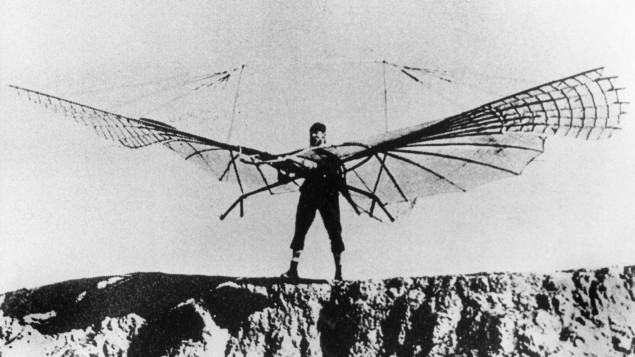
\includegraphics{otto_lilienthal}
    \caption[]{|OR| and |XOR| operations visualized. The |XOR| problem cannot be solved by drawing a single line.}
    \labfig{XOR}
\end{marginfigure}

As it has been explained in the previous section, the perceptron is equal to a binary linear classifier.
As such, the perceptron can only classify linear separable data perfectly.
Since the |XOR| problem can obviously not be solved with a straight line separating the two classes, the perceptron is also not able to compute such an operation. 

This realization led to the first decline in interest in artificial neural networks.

Since then there have been ways of solving this problem for SVMs by projecting the data into a higher dimensional space.
Another approach kept the logic as is but went from the existing shallow network approaches to deep neural networks (DNN).
\textbf{Deep Neural Networks (DNN)} are ANNs which consist of more than one hidden layer.
A single perceptron may not be capable of computing |XOR| but it is capable of calculating |AND|, |OR| and their negated forms.
By using one perceptron with two units to compute |AND| and |OR|, a second layer perceptron can use compute |XOR|
\begin{align}
    XOR(x, y) = AND(OR(x, y), NOT(AND(x, y)))
\end{align}

Now, the |XOR| problem becomes solvable.

\marginnote{The ability to stack multiple layers in ANNs stems from discovery of backpropagation which shall be explained in \refssec{backprop}.}

As before only linear functions could be approximated by perceptrons, multiple layers of perceptrons allow for any higher degree function to be approximated as well.
Thus, \textbf{Multi-Layer Perceptrons (MLP)} sparked new interest in the field of artificial neural networks.

This interest also originated in the similarly layered structure that has been found in the brain.
\begin{marginfigure}
    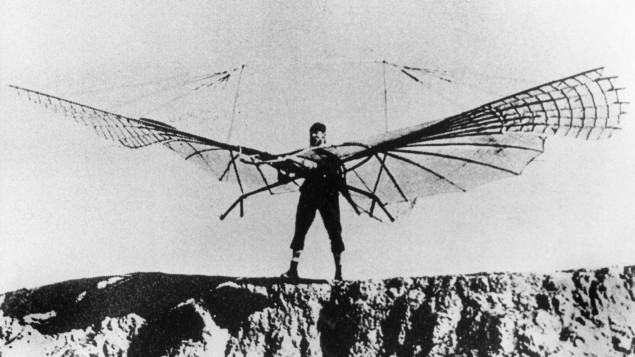
\includegraphics{otto_lilienthal}
    \caption[]{The brains structure under a microscope}
    \labfig{brain}
\end{marginfigure}
\begin{marginfigure}
    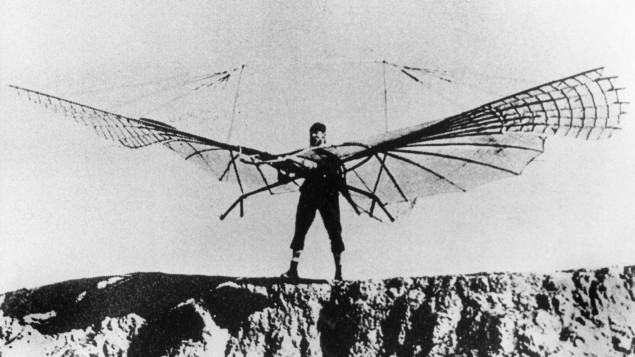
\includegraphics{otto_lilienthal}
    \caption[]{Layers of an MLP}
    \labfig{MLP}
\end{marginfigure}
Ultimately, MLPs really start to show the connected structure in a network that is typically expected.

MLPs are also called \textbf{fully connected networks} since each unit is connected to all unit in the previous layers as well as all units in the next layer.

%\marginnote{This new connectedness opens a realm to a whole field of studies on graphs, networks and network motifs \cite{network_motifs}.}

%histrocal rollercoaster of interest (AI winter) ?
%limited capabilities of the perceptron for XOR problem
%use either higher dimensional input -> kernel trick or stack many perceptrons
%any 2 layer MLP can approximate any continuous function (or somethign like that)
%simialrity to network motifs, make a large network of many identical pieces
%similar to how the brain works as well.

\subsubsection{Activation Functions}
%linear algebra shows that any linear function can approximated by just two perceptron layers for a linear activation function -> more layers do not make sense.
These newfound capabilities for MLPs are not only restricted to binary operations but will translate into continuous space.
In this case the hidden-layer perceptrons get stripped of their activation function.
The activation function of a perceptron has been used up until now to make a class prediction $y$ from the score $z$, which is also called pre-activation.

Replacing the step function with a linear activation function (\ie identity function), each hidden-layer's perceptron would initially seem to increase the capabilities of the MLP.
Unfortunately, this is not the case as any subsequent perceptrons with linear activations can be reduced to a single preceptron.
\begin{align}
    \vec{z}_2 = \mat{w}^T_2 \vec{z}_1(\vec{x}) = \mat{w}^T_2 \mat{w}^T_1 \vec{x} = \mat{w}' \vec{x}
    \labeq{LAF}
\end{align}

Consequently, the step-function that was used in the |XOR| problem played an important role.
The reason for this is the non-linear nature of the step-function in contrast to any linear activation function.
It can easily be shown, that \refeq{LAF} does not hold for non-linear activation functions.

Thus, the question becomes which other activation functions there are that go beyond binary classification.
An early popular choice are sigmoid functions (logistic function or $\tanh$).
Especially the logistic function is popular due to its similarity to the step-function amongst other things.
\begin{align}
    \sigma(z) = \frac{1}{1 + e^{-z}}
\end{align}
\begin{marginfigure}
    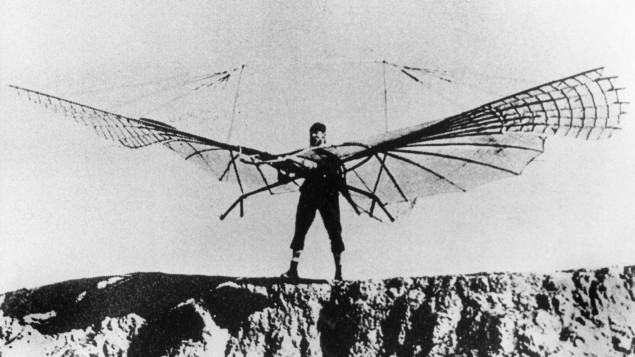
\includegraphics{otto_lilienthal}
    \caption[]{A sigmoid function. It saturates to $1$ for very large inputs and $0$ for very small inputs, similar to the step function.}
    \labfig{sigmoid}
\end{marginfigure}

Another popular choice are rectified linear units (ReLU) which are identical to a linear activation for $z > 0$ but mimic the step function for $z < 0$.
Basically, a ReLU suppresses the signal of a perceptron until it reaches the threshold of $0$ and then forwards the signal unaltered.

Another activation function 'leaky ReLU' attenuates the signal below the threshold with a factor $\alpha$ instead of fully suppressing it.
\begin{marginfigure}
    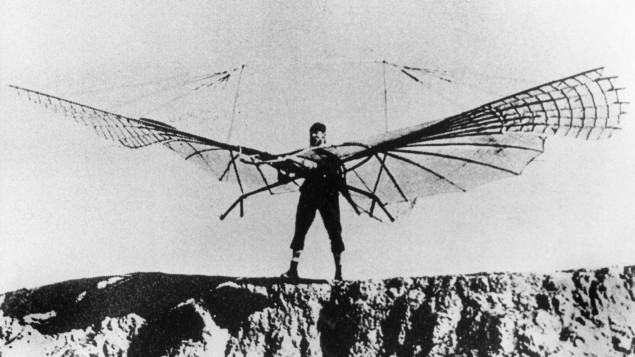
\includegraphics{otto_lilienthal}
    \caption[]{ReLu activation function}
    \labfig{relu}
\end{marginfigure}
\begin{marginfigure}
    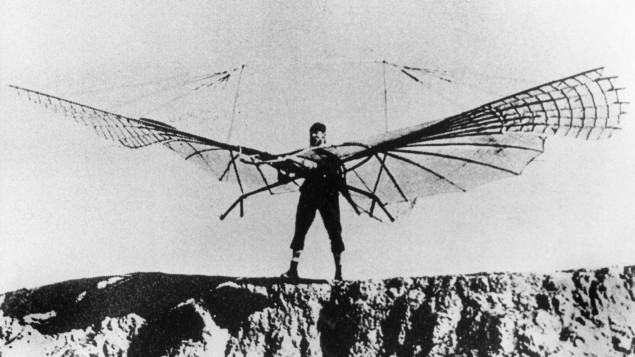
\includegraphics{otto_lilienthal}
    \caption[]{leaky ReLu activation function with $\alpha = 0.2$}
    \labfig{lrelu}
\end{marginfigure}


%move on from step function as activation
%Activation functions have already been used to describe the perceptron and the artificial neuron by McCulloch and Pitts.
%In both cases (as well as the binary linear classifier) the inputs are weighted and summed up to something called a \textbf{pre-activation} \cite[p.~6]{GrosseNotes}.
%The pre-activation is then checked against a threshold which is often $0$ if there is a bias term involved.
%In all previously given cases this decides whether a unit becomes active or which class the input is allocated to.
%\begin{align}
%    \sigma(z) = \frac{1}{1 + e^{-z}}
%\end{align}
%
%There are many more activation functions with different properties such as the \textbf{sigmoid activation} $\sigma$.
%\begin{align}
%    \sigma(z) = \frac{1}{1 + e^{-z}}
%\end{align}
%$\sigma$ is also inspired by nature as a neuron can fire at different rates according to its input.
%Even though this is very much simplified, the main idea is, that a strong input ('mentioning 'weightloss' hundreds of times) should lead to a strong output ('this mail is definitley spam').
%
%\reffig{sigmoid} shows that the output $\sigma(z)$ scales with the input $z$ but saturates for both very large and very small $z$.


%inability to solve XOR problem
%thus stack multiple 
%non-linearity is important 

%hiddenlayers

%After motivating the perceptron, this section will focus on combining multiple layers of perceptrons, which make up the \textbf{multi layer perceptron (MLP)}.
%The MLP combines several perceptron layers in series which is the first step towards what is described as deep neural networks.
%In a first thought experiment the original input layer and the output layer shall be separated by an additional layer that works quite simialrly to the input layer.
%Instead of receiving a signal 'from outside' the added layer takes the input layer's activations as a new input signal ....

%two or more hidden layers -> deep neural network
Deep neural networks repeat the step from the previous section over and over again which results in a \textbf{deep} architecture, where deep refers to the number of layers....


\section[Convolutional NNs]{Convolutional Neural Networks}
\subsection{Convolutions}
%advantage of convolutions as they use fewer weights
%unified behavior over space -> invariance


%process information hierarchically
%each layer is a collection of image filters

%mathematical explanation of what a convolution does
\subsection{Normalization}
%Motivate by facilitating training or look into book
Ioffe and Szegedy introduced BN to ease training of feed-forward networks.
affine parameters $\gamma$ and $\beta$

\subsection{Regularization}
%addition to loss but just keep training on track


%\setchapterpreamble[u]{\margintoc}
\chapter{Generative Models}
\labch{GenModels}
\todo{think about including htis into previous chapter as well as optimization -> save some space?}
After the previous two chapters focused the basic ideas and mathematics behind neural networks, this chapter will introduce basic architectures and building blocks of many recent neural networks.
Not every new publication reinvents the wheel
most works nowadays rely on established architectures and losses and only change parts of these
introduce some common language and concepts in CV

\section{Discriminators \& Classifiers}
Discriminators and Classifiers are some of the most basic structures
Discriminators often act as binary classifier
also as critiques, how well does this fit?

classifiers tend to classify mutliple classes
one-hot encoding
softmax loss

both structures are subject to challenges such as imagenet
perform better than humans nowadays \cite{something}
one very popular structure is that of VGG with ImageNet weights
many classes and lots of natural images
other architecture is resnet with its residual blocks

\section{Generators \& Decoders}
given some low-level input, decoders/generators 
words are often used interchangebly, sometimes generators generate content from noise see next section, decoders specifically decode low-level information into specific high-level representation 1-to-1 pairing exists.

very often use inverted VGG architecture
hard to train if paired data is not available

\section{Autoencoders}
Autoencoders are combiantion of encoders which are very simialr to classifiers and decoders in row
main goal is reconstoruction 
other goal is feature space which should have some nice properties
E.G change somehting in feature space and look at reconstruction what happens
position in feature space should represent something in image space as well
have some specific losses for this -> metric learning(jsut reference it)

\section{Generative Adversarial Networks}
GANs \citeauthor{GAN} \cite{GAN} are a combination of generator and discriminator
\marginnote{SChmidhuber claims its his idea, cite him to be on the safe side}
generate sample from noise
discrimiantor judges sample (does it fit into the distribuion that the discrimiantor has been shown so far/expects)
equillibrium problem

got the Turing award and is one of THE major gamechangers in the last decade
many applications such as AIs driving or alpha Go more or less are based on this principle

\subsection{RS- \& RA-GAN}
is used in this paper thus explain it


\subsection{Flavors of GANS}
condition genration on some input liek decoder cGAN
improve loss funciton WGAN
combine with autoencoder AEGAN
MSGGAN and ProGAN
jsut some ideas...



%\setchapterpreamble[u]{\margintoc}
\chapter{Artistic Computer Vision}
\labch{ACV}
This chapter shall dive into existing and related work that combines computer vision with artistic content.

Applying computer vision techniques to images with artistic content has been interesting and challenging at the same time.
Due to the often observed change in appearance that can be observed for many artistic images, existing CV pipelines for \ie classification usually do not work as intended.
This makes it all the more interesting to see, how these pipelines are affected by this domain gap.

At the same time artistic images bring something into the mix which 

%in SBR stroke is the basic unit texture synthesis fills each pixel individually.

%non-photorealistic rendering vs. photrealism
%clesly realted to texture synthesis and transfer
%games and movies benefit from this
%since the 1990's starting with artistic rendering of images (paint by numbers)

%with neural network more practical applicatin of style transfer have become popular:
% - funny iphone filters
% - translating images between other domains (google maps, satelites etc.) -> many possible applications
% quantitative style (materials used, color shoice etc.)
% qualitative style (how are people drawn etc.)

% historically there have been many different approaches
%try to group these approaches on the problem formulation and the approach

%color choice
%how to display something (is it unnaturally large or small ...)
%direction of brush strokes
%choice of material
%which details are kept which details are lost?

%all of this together makes style

%usually style transfer formulates this much simpler (maybe see gatys formulation?):
%create something that maintains the orginal content to some  degree but people would categorize together with other works of that 'style'
% style is rather something by what art can be grouped together 'easily'


\section{Problem Formulation \& Approach}
The problem that style transfer might seem easy to capture at first, but it quickly becomes harder when trying to formulate it.
As 'style' is simply defined as "a typical way of doing something", it includes actually all aspects 

%style transfer
%create IMAGE that catches style as well a possible, doesn't rally matter how, the pixel should make sense in the end

%painterly rendering
%create something that looks like is has been drawn with a paint brush (or any other such tool, e.g. has some gloss to it etc.)
%don't really concentrate on deeper style but just the apprearance

%drawing networks
%do not care as much about the apprearance or the style but how to compose the image in a different parameter space, FAST

%brush stroke extraction and image analysis
%get more information about the image, that can help to classify it, or identify it. Do not get all brush strokes but those that are characteristic

%drawing networks and painterly rendering are really much of the same with different focus on what matters.


%this work would fall into painterly rendering territory paired with brush stroke extraction


%features of DNN have been used to classify paintings

\section{Brushstroke Extraction}
%no updates in recent years
%relatively small field
%shift towards creating art rather than analyzing it
%what to do with the data besides identifying forgeries?


\section{Painterly Rendering}
\labsec{PR}

%refer to painterly rendering review

Painterly rendering is a field of computer vision that focusses stylization of images on giving the impression that certain tools were used.
Most often this would be the looks of pencil drawings or brush stroke paintings as these looks are very distinctive.

The use of such techniques often comes with a layer of abstraction which painterly rendering approaches often enforce explicitly though parameters.
One could see this as a hard regularization.
This is the reason why painterly rendering is rarely compared to style transfer (see next section) as style transfer achieves this abstraction more implicitly.
For instance, an impressionistic style is often achieved by limiting the length and width of brush strokes.
Nonetheless, the focus really lies on explicitly formulating an algorithm to transform images to something that looks like a painting.

There are several different key approaches how to achieve this, which shall be presented chronologically.

The earliest approaches were stroke-based renderings, which artificially generated single strokes.
With such strokes at hand the challenge mainly was to either improve the quality of these strokes or improve the algorithm which aligns them.
This field is especially close to the approach of this thesis.

In filter-based rendering filters are used to give the impression of \ie paint on canvas.

Lastly, drawing networks revived stroke-based rendering with modern machine learning techniques.
The focus of this field is really to remove the tuning of parameters and imitate the way humans would draw.
%Along this discrepancy comes a shift in focus.
%Style transfer wants to create something that looks like a photo of a painting by a certain artist.
%At the same time painterly rendering focusses on imitating the real world and produce an output that looks like it has been drawn by hand.
%One could say, that style transfer is about the broader picture and painterly rendering cares more about the details.
%
%As the goal is always just reconstruction an image as good as possible with the regularization at hand the target style can only formulated very broadly, like 'pointillism' or 'painting'.
%Any control over the painting beyond that is really hard to realize.
%
%On the other side, the resulting representation can come in a parametrized form, such that the image can be brought into a different domain.



\subsection{Stroke-Based Rendering}
%FOCUS ON PLACING STROKES
%two step approach: approximate and render -> flawed since the rendering matter for reconstruction.
%SBR creates images by placing strokes according to some goals.
%the tricky part is to define an objective function because the reconstruction is always in there
%two approaches: greedy algorithms (genetic algos) and optimization alogrithms \cite{hertzman}

%early painterly renderign techniques basically try clustering pixels with different mehtods and then repcaling them with regular shapes like stipples and tiles.
%voronoi algorithms cannot really take color into account but just create and even spacing with some constriants.

%trial and error alogrithms perturb a given set of strokes repeatedly and revert the changes if they result in a worse image.
%Haeberli first introduced such an algorithm  (paint by numbers)


%greedy algorithms predict a stroke and then leave it
%greedy algorithm is optimiation based
%paint x numbers Haeberli was the first to leave placing brush strokes to the user/artist and details of the brush strokes ar determined automatically
%Other followed suit and automated this procedure.


%other review
%these properties are of interest position and density, path and orientiation, lenght and width, ordering, color, temporal coherence
%renderign abstract the input uniformly


%the orientation of strokes is really quite often just perpendicular to the gradient in the image
%- arbitrary for large homegneeous color fields -> use some tricks to tackle this problem

%length and width of style are often just a parameter that is loosely motivated as a style like impressionism
%longer strokes by hertzman are just joint shorter staight strokes
%superquadrics are used by COllomosse and Hall

%order
%hertzmann was first to order strokes according to their thickness -> start with thick background strokes and then come up with smaller foreground strokes
%standard procedure is using low-pass fitlers and then generating mutiple layers
%collomosse and hall ordered according to salience map

%color
%color is often just the average of the pixels or just the color at the centroid.
%others use predefined palettes or color datasets for artists

%some want temproal coherence for 'animated paintings'

Stroke-based rendering focuses on generating real-looking brush strokes and composing images with these.
Two aspects which shall be of importance in this thesis as well.

\citeauthor*{paintbynumbers} introduced stroke-based rendering with his seminal work \citetitle{paintbynumbers} \cite{paintbynumbers}.
In this work he presents two methods which would allow for reconstructing images in an abstracted representation.
His first approach is interactive and requires a user to click a certain points in an image to place a brush stroke there.
Then his software would automatically select a brush stroke color and size.
He proposed several ideas on how to align the brush strokes on the canvas.
Either users could do this on their own, or the orientation would be perpendicular to either the global gradient (uniform alignment) or local gradient (non-uniform alignment) of the image.
\begin{marginfigure}
    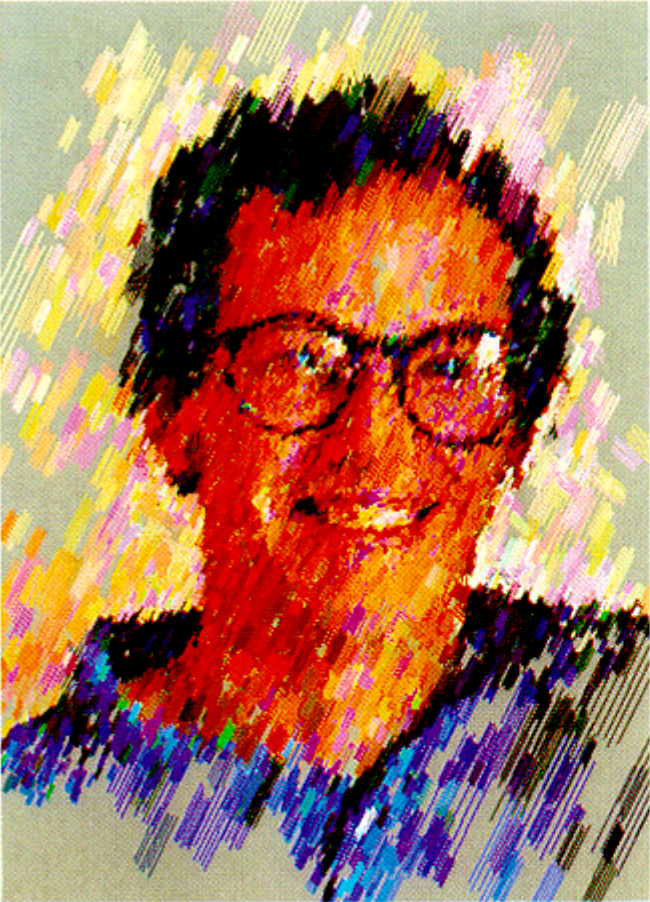
\includegraphics{haeberlihandcrafted}
    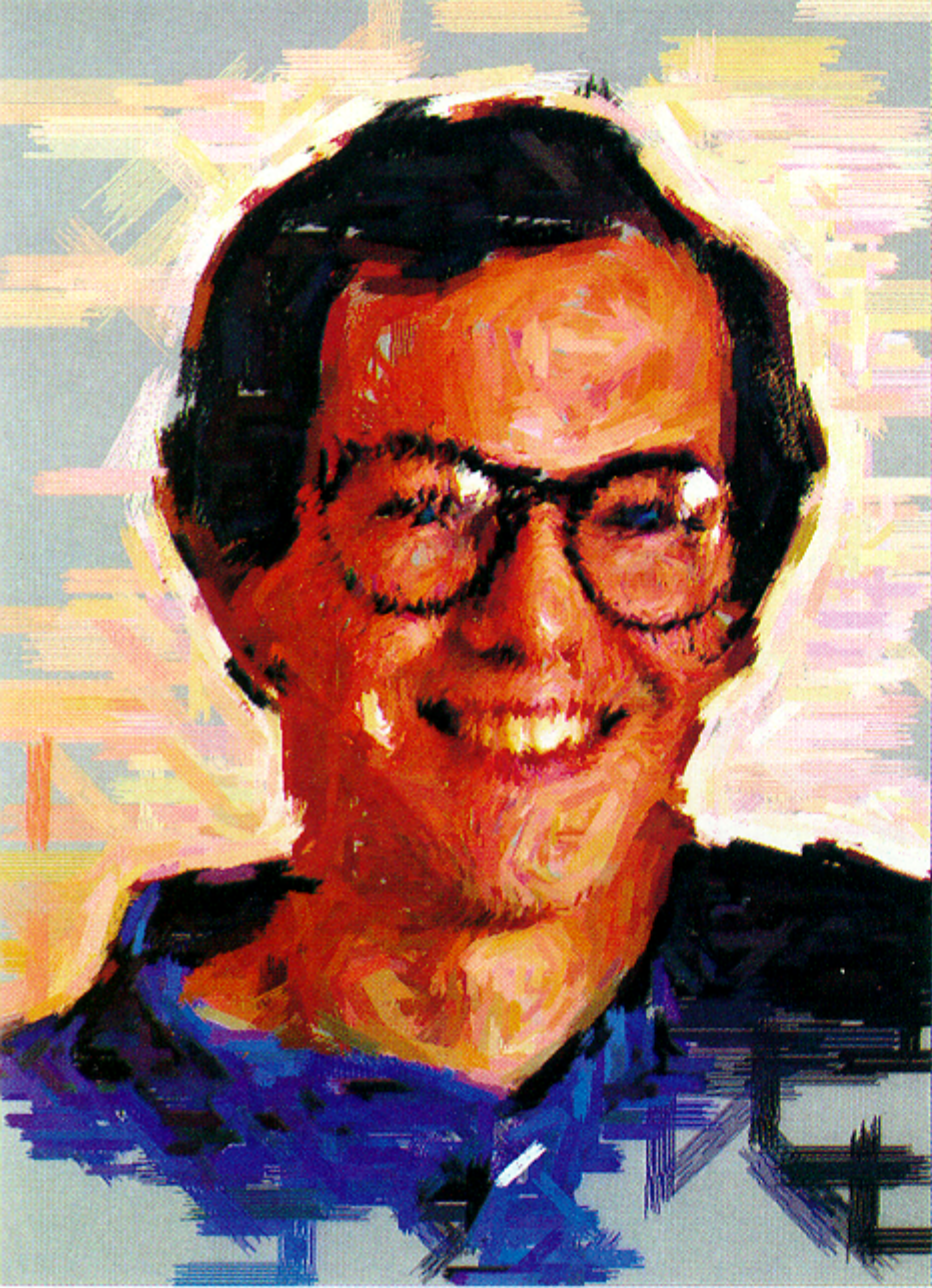
\includegraphics{haeberligradientdriven}
    \caption[]{Interactively painted images using \citeauthor*{paintbynumbers}'s method with a hand-selected orientation (\reffig{handselected}) and a gradient-driven orientation(\reffig{gradientdriven}).}
    \labfig{haeberliportrait}
\end{marginfigure}
\citeauthor*{paintbynumbers} even introduced the use of a scanned brush stroke texture in his algorithm.
\begin{marginfigure}
    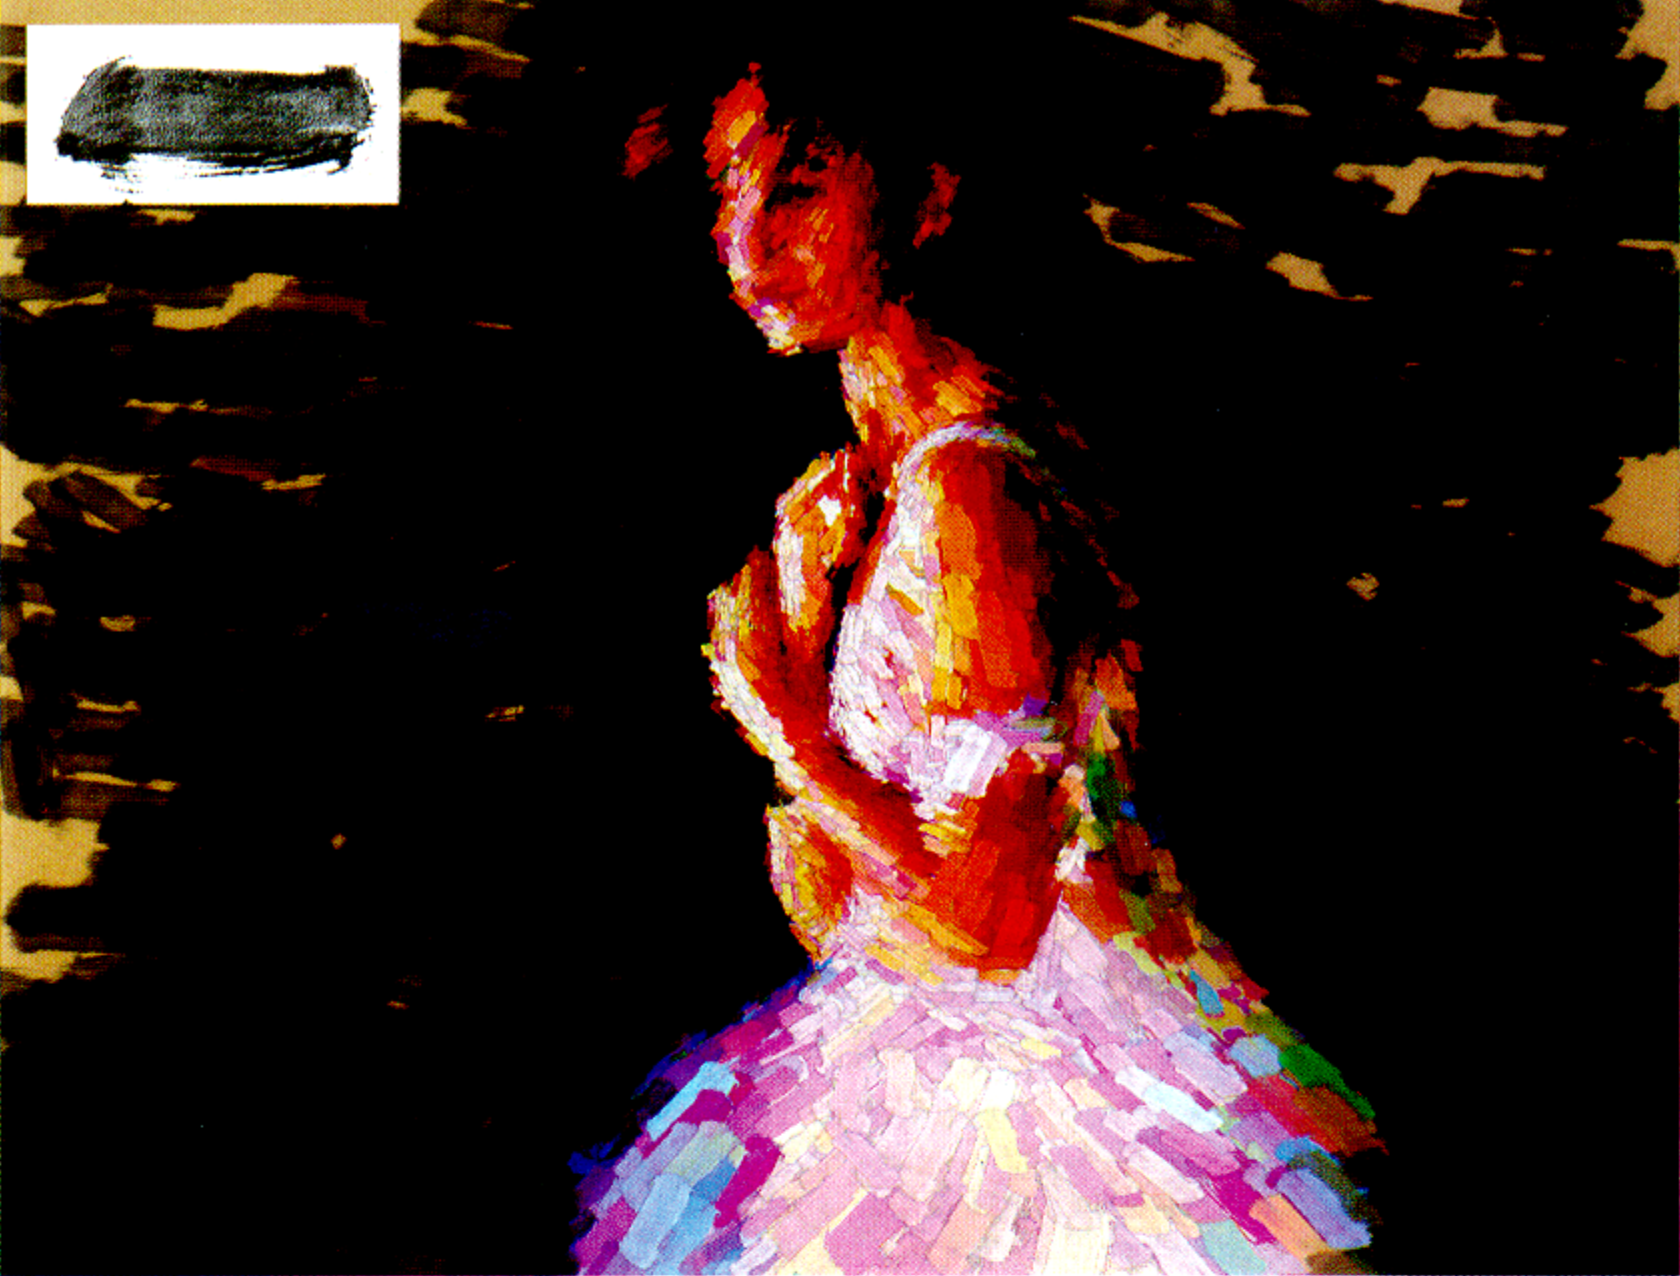
\includegraphics{haeberlibrushstroke}
    \caption[]{Rendered image with a brush stroke texture}
    \labfig{haeberlitexture}
\end{marginfigure}

Additionally to his interaction-based approach, \citeauthor*{paintbynumbers} also introduced a relaxation based approach \cite{paintbynumbers}.
In this approach a given set of 100 brush strokes is iteratively perturbed.
If the perturbation minimizes the energy function (L2-distance), the perturbation is kept.
If not, another perturbation is applied.
\begin{marginfigure}
    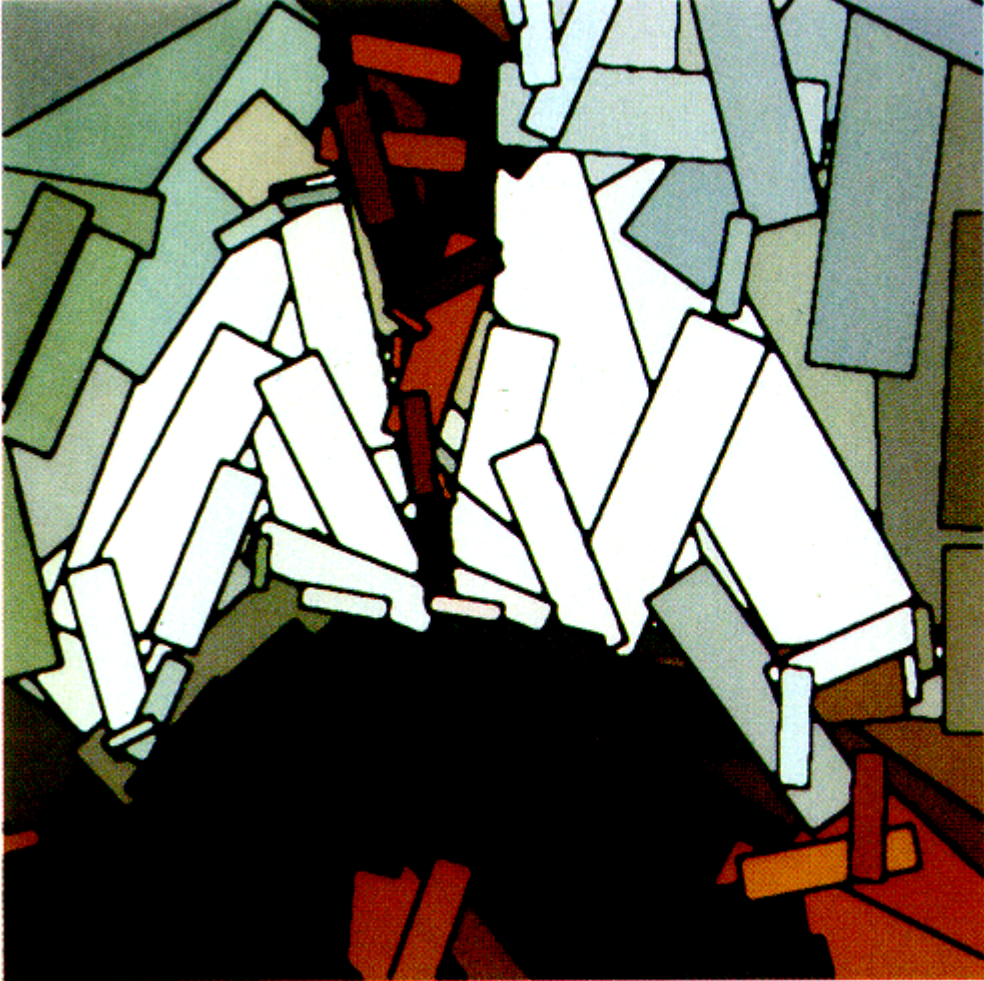
\includegraphics{haeberlirelaxation}
    \caption[]{Image approximated by relaxation.}
    \labfig{haeberlirelaxation}
\end{marginfigure}
This is described by \citeauthor*{hertzmannreview} as trial-and-error algorithm and very similar to genetic algorithms which shall be explained later \cite{hertzmannreview}.

Based on \citeauthor*{paintbynumbers}'s work, other authors automated the process of stroke positioning.
At the same they improved various aspect of brush strokes which were well categorized in a review by \citeauthor*{PRreview}.
The relevant categories are position, path and orientation, length and width, ordering, and color \cite{PRveview}.

%litwinowicz
\citeauthor*{apple} proposed a straight-forward way of placing brush strokes evenly spaced over the entire image.
Parameters are then inferred similar to \citeauthor*{paintbynumbers}'s approach.
To give a more random feel to these brush strokes, the obtained parameters are randomly perturbed according to preset parameters.
Also, a weakness of orienting brush strokes perpendicular to the gradient is dealt with.
For large uniform areas with little to no gradient, the orientation could become arbitrary.
\citeauthor*{apple} proposes to refine the gradient field by interpolating between the boundaries of large uniformly colored areas.
Also, \citeauthor*{apple} introduced temporal coherence to brush strokes, which meant that brush strokes move with the optical flow between frame in a video.

%hertzmann
\citeauthor*{hertzmann} reformulated the problem as an energy minimization problem in two publications \cite{hertzmanreview, Hertzmann}.
\begin{align}
    E(R) & = E_{\text{recon}}(R) + E_{\text{area}}(R) + E_{\text{nstr}}(R) + E_{\text{cov}}(R) \\
    E_{\text{recon}}(R) & = \sum_{x \in W, y \in H} w_{\text{recon}}{}_{x, y} \norm{I_{x, y}(R) - I_{x, y}}^2_2 \\
    %E_{\text{area}}(R) & = w_{\text{area}} \sum_{r \in R} \text{area){r} \\
    %E_{\text{nstr}}(R) & = w_{\text{nstr}} (\text{\#R}) \\
    %E_{\text{cov}}(R) & = w_{\text{cov}} (\text{\#empty pixels in $I(R)$}) \\
\end{align}
where $R$ is a brush stroke representation, $I$ is the target image, and $I(R)$ is the rendered representation.
$x$ and $y$ are pixel positions.
By adjusting the different weights, properties of the rendering can be altered.
$w_{\text{recon}}$ can vary spatially and dictate how well the reconstruction must fit the original image in certain areas.

Additionally, he added long strokes as B-splines with arbitrary control points.
In contrast, \citeauthor*{paintbynumbers} and \citeauthor*{apple} argued that short straight brush strokes would aid the perception of impressionistic style.
Furthermore, \citeauthor*{Hertzmann} added advanced rendering for brush strokes with synthetic textures in his work \cite{Hertzmann}.

\citeauthor*{Hertzmann} combined all these aspects in his approach with advanced relaxation methods similar to \citeauthor*{paintbynumbers}.
Based on trial-and-error search, \citeauthor*{Hertzmann} samples a local region along the many dimensions that represent a single brush stroke.
The best set of parameters that minimizes the energy function $E$ is then picked as new parameters.

In order to achieve better visual quality \citeauthor*{Hertzmann} also employs a coarse-to-fine multi-layer rendering approach.
Hereby, he blurred the image in the early iterations of his method and fixed the brush size at a large value.
Blurring of the image would then be gradually reduced along with the brush size.
The final implementation is further optimized to accelerate the relaxation algorithm and allow for more brush strokes than \citeauthor*{paintbynumbers}'s approach.

Ultimately, \citeauthor*{Hertzmann} achieves respectable results with his approach and many ideas of this thesis can be found in his works as well.

\subsubsection{Stroke Rendering}

%FOCUS ON QUALITY OF STROKES
%physical simulations
%Lee et al, baxter et al focused on 3D version of bristle

%there are papers which focus on the material i.e. paper etc.

%later



\subsection{Filter-Based Rendering}
%IMAGE PROCESSING BASED TECHNIQUES
Parallel to his works in stroke-based rendering, \citeauthor*{imageanalogies} proposed a way of stylizing images much faster by using trainable filters.
They call their technique 'image analogies' since the transformation between two training images is analogously applied to a test image.

Basically, for creating the impression of brush strokes a photograph $A$ and a painting of that photograph $A'$ is needed.
As this is rarely the case, \citeauthor*{iamgeanalogies} showed that using anisotropic diffusion works also reasonably well to generate $A$ from $A'$.
Then their algorithm searches locally for the best filter parameters $F(p)$ that transform $A(p)$ into $A'(p)$.
$p$ is an arbitrary position in the image.
By using another search algorithm to match similar regions $B(p)$ and $A(p)$, $F(p)$ can be used to transform $B(p)$ into $B'(p)$.
Thus $B'$ a stylized version of $B$ can be obtained by transforming it analogously to $A \rightarrow A'$.
%Hertzmann et al 2010 smooth a painting and optimize filter parameters for the inverse transformation -> apply the filters to photos
    %similar to superresolution and texture synthesis
%first approach is just grouping pixels simialrly to super-pixels
Other works like \citeauthor*{texturetransfer}~\cite{texturetransfer} have built on this principle idea which has led to a fast texture transfer algorithm \cite{fasttexturetransfer}.
Besides only matching local region according to their pixel values, \citeauthor*{texturetransfer} obtain a flow map (which they call 'directions'), that is based on the content image's gradient.
This flow is then also matched against the style image.
\begin{figure}
    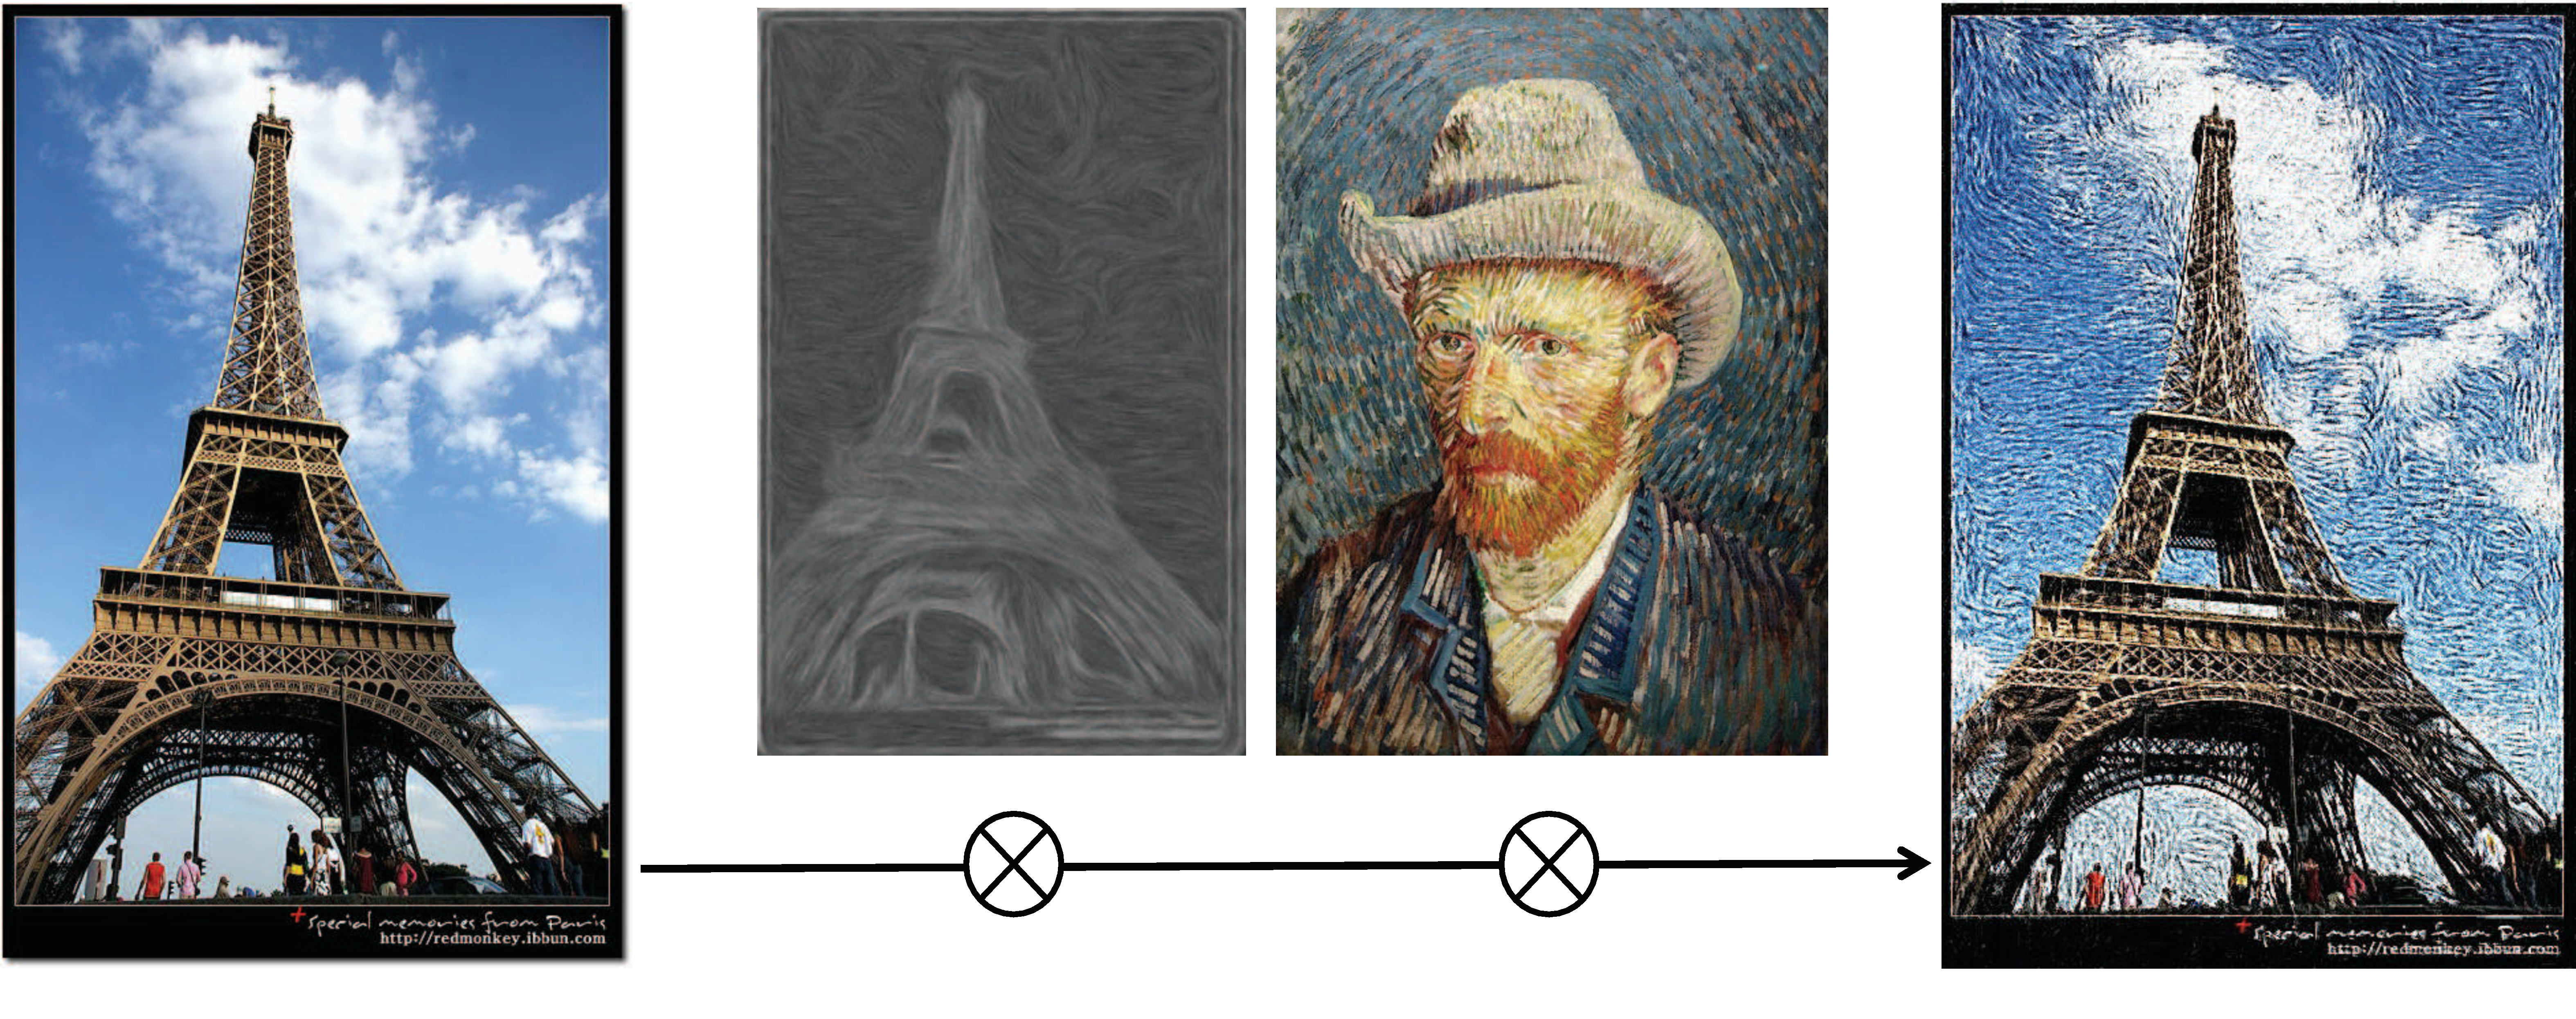
\includegraphics{texturetransfer}
    \caption[]{Target image $T$ is combined with a dictional map specially obtained from $T$ and a style image  $S$. The result maintains the direction's flow while presenting the texture from $S$.}
    \labfig{texturetransfer}
\end{figure}

%Lee et al 2010 transfer the texture of brush stroke onto an image much like style transfer (this is the intersection)


\subsection{Drawing Networks}
%gaining traction

%were described by hertzmann as greedy algorithms.

%learning2Paint
%SPIRAL
%DrawNet
%PaintNet


%image transofrmation tasks denoising, colorization, super-resolution, semantic-segmentation, depth estimation, 

\subsection{Genetic Algorithms}
Genetic algorithms are typically not closely associated with painterly rendering, even though they represent just a different approach to algorithms for this problem.

Genetic algorithms already perform a similar task in order to approximate images by other geometric shapes or even smaller photos (also known as the popular photo mosaic effect).
Starting with a random set of circles that are parameterized by their position, radius, and color, it then chooses the most successful samples and resamples in a region around these.
This process is repeated until a certain level of convergence is reached.

%refer to neural style transfer: a review

\begin{marginfigure}
    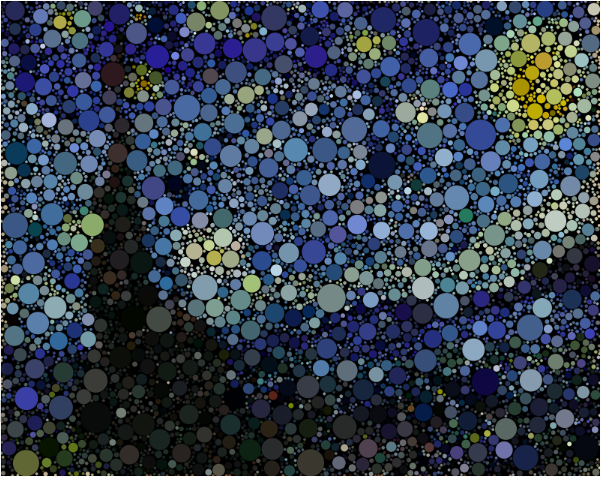
\includegraphics{genetic_starry_night}
    \caption[]{Starry Night approximated by a genetic algorithm using only circles. \url{https://effyfan.com/2018/03/02/w6-van-gogh-flowfield/}}
    \labfig{genetic}
\end{marginfigure}

As well as this does work, it is very much computationally expensive as most samples will not fit the image, thus searching for the small set of fitting shapes requires to evaluate all the wrong shapes as well.
Considering artworks, brushstrokes have many more degrees of freedom, and artworks usually consist of upwards of a few thousand brushstrokes.
Consequently, it would be considerably more challenging to apply to this problem until computational resources have become a few magnitudes more powerful.

\begin{figure}
    \includegraphics{photomosaic_starry_night}
    \caption[]{Photo mosaic of Starry Night using only images by the Hubble Space Telescope. \url{http://www.astro.uvic.ca/~alexhp/new/figures/starrynight_HST.001.jpg}}
    \labfig{photomosaic}
\end{figure}

\section{Style Transfer}
\labsec{ST}

This field of style transfer has its origins 
%most active field
%style and texture are similar problem

\subsection{Early Approaches}
Earliest approaches
%painterly rendering is some kind of style transfer but shall be dealt with explicitly
%focus is on approaches that work only with pixels
%filters
%texton based approaches

%Some early approaches include histogram matching on linear filter responses [19] and non-parametric sampling [12, 15].
%       . Pyramid-based texture analysis/synthesis
%       Split and match: example-based adaptive patch sampling for unsupervised style transfer
%       Image quilting for texture synthesis and transfe
%low-level statistics and fail to perceive semantic structures



\subsection{Neural Style Transfer}
%A bit similar to transfer learning -> utilize the pretrained features especially of the early layers.
The field of style transfer has really gained traction in 2015 with the publication of \textbf{A Neural Algorithm for Artistic Style} by \citeauthor*{gatys}.
It was the first approach to transfer the style of one image to another and at the same time maintaining a high contextual fidelity.
In retrospective, this work really kicked off neural style transfer as a field.

\citeauthor*{gatys} themselves pinpoint the novelty of their approach as 'manipulations in feature spaces' as opposed to previous approaches that 'directly manipulate the pixel representation of an image'\cite{gatys}.
They use existing neural architectures and extract information in two separate ways, such that content and style can be separated.

Previous works already used \textbf{perceptual loss} to accumulate information on the content in an image \cite{percep_loss}, or check whether two images have the same content \cite{other_percep_loss}.
%networks trained on object recognition increasingly care about the content with every layer
Perceptual loss is based on the VGG-19 architecture \cite{VGG} which is a deep CCN trained for object classification on ImageNet \cite{imagenet}.
By arguing that the network's layer activations increasingly respond to the content when following the networks' hierarchy.
Some much even, that it is possible to reconstruct the content of an image by using the activations of one such layer.

For reconstruction of an image's content, gradient descent is performed on a white noise image.
The gradient descent aims to minimize the perceptual distance between the reconstruction and the target image.
Perceptual distance is defined as the L2-distance between the activations of two images in deep layer of the VGG-network.

For image vector $\vec{x}$ with $\vec{x} \in = \R^{M_0}, M_0 = H_x \dot W_x $, a layer $l$ of the network has $N_l$ feature maps of size $M_l$.
In this case $M_l$ is equal to the height times the width of the feature map of the $l$-th layer.
The activations of the $i$-th filter ($i \in N_l$) at position $j$ ($j \in M_l$) at layer $l$ can then be represented by matrix $F(\vec{x})_{ij}^l \in \R^{N_l \times M_l}$.
The perceptual distance is then defined as
\begin{align}
    d_{\text{percep}}(\vec{x}, \vec{y}) = \sum_{i, j} (F(\vec{x})_{ij}^l - F(\vec{y})_{ij}^l)^2 = \norm{\tensor{F(\vec{x})}^l - \tensor{F(\vec{y})}^l}_2^2
\end{align}
, which allows to define the perceptual loss or content loss as 
\begin{align}
    \L_{\text{content}} = \frac{1}{2} \sum_{i, j} (F(\vec{x})_{ij}^l - F(\vec{y})_{ij}^l)^2 = \frac{1}{2} \norm{\tensor{F(\vec{x})}^l - \tensor{F(\vec{y})}^l}_2^2
\end{align}

\marginnote{The factor $\frac{1}{2}$ will cancel out when deriving $\L_{\text{content}}$ with respect to $F(\vec{x})_{ij}^l$.}

Minimizing the content loss between two images, by using gradient descent the content of an image can be restored (see \reffig{content_style_loss}).

\begin{figure*}
    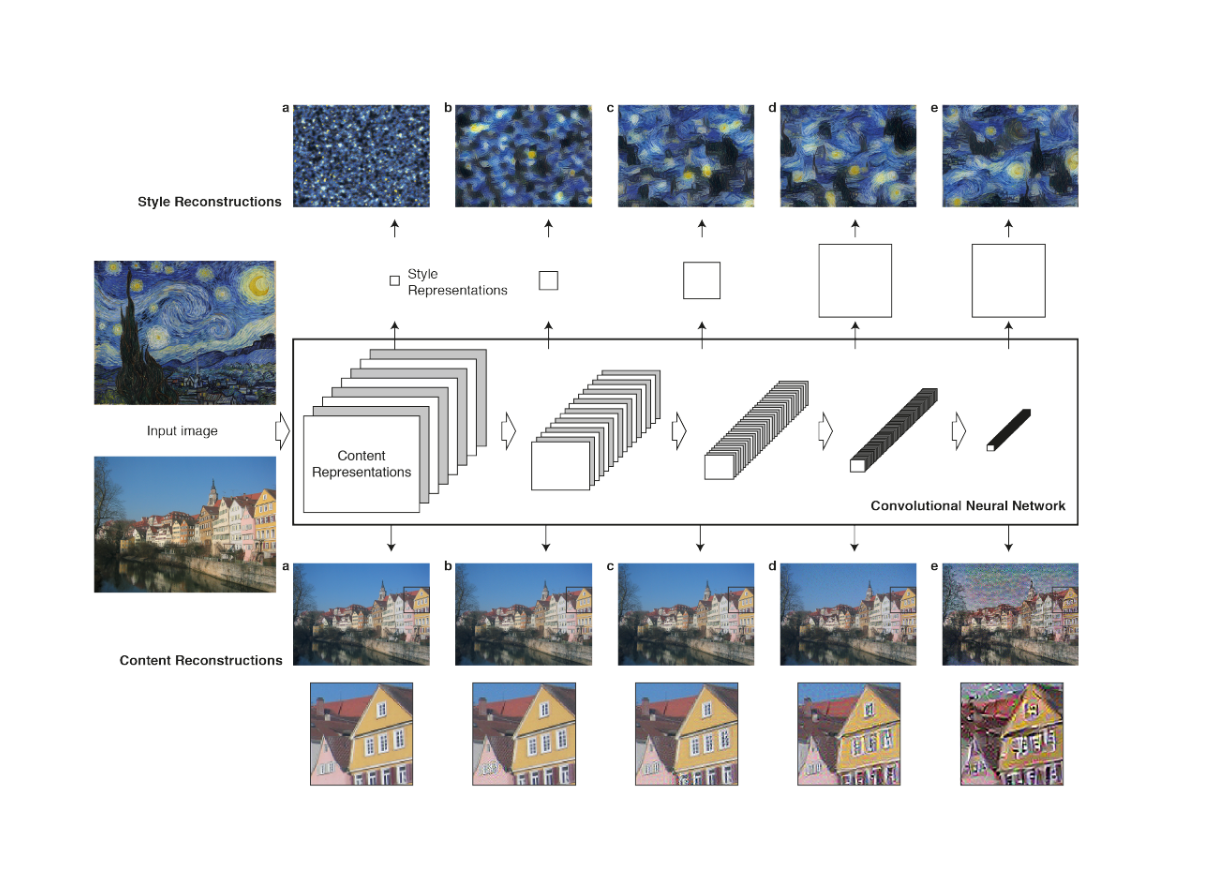
\includegraphics{content_style_loss}
    \caption[]{Reconstructions of content(bottom) and style(top) using different layers. \cite{gatys}}
    \labfig{content_style_loss}
\end{figure*}

As approximating the content of an image has now become possible, the question is whether this is possible with style as well.
\citeauthor*{gatys} again turned to the pre-trained VGG network for this.
They explicitly reduce style to texture for this reason and thus search for a feature space that captures \textbf{texture} rather than content.
Subsequently, \citeauthor*{gatys} propose the use of \textbf{Gram matrices} as they capture the correlations of feature-activations over their spatial extent.

The Gram matrix of a given matrix $\tensor{A}$ is the inner product of all column vectors in $\tensor{A}$.
\begin{align}
    G = \langle a_{i}, a_{j} \rangle = \tensor{A}^T \tensor{A} \text{ if $a_1$...$a_j$ are column vectors of $\tensor{A}$}
\end{align}
The resulting Gram matrix G now has the form $j \times j$ and captures texture information but no longer the global content.

\refsec{problem} already mentioned that style is very complex and exists at various scales at the same time which \citeauthor*{gatys} address by using many layers.
As these layers sit at different depths their field of view varies and each layer captures information at a different scale.
Early layers will tend to hold small scale information, later layers will hold larger scale information with every layer.

\citeauthor*{gatys} first compute the Gram matrices each layer $l$ for both the target style image and the current image.
Then they use the L2 distance metric to measure the discrepancy between them.
\begin{align}
    G(\vec{x})^l & = \frac{1}{(2 N_x^l M_x^l)^2} F(\vec{x})^l{}^T F(\vec{x})^l \\
    G(\vec{y})^l & = \frac{1}{(2 N_y^l M_y^l)^2} F(\vec{y})^l{}^T F(\vec{y})^l \\
    d_{\text{style}}^l(\vec{x}, \vec{y}) & = \norm{G(\vec{x})^l - G(\vec{y})^l}^2_2 \\
\end{align}

\marginnote{The denominator of $\frac{1}{4 N_x^l{}^2 M_x^l{}^2}$ is squared since the Gram matrix is the product of a matrix with itself transposed.}

The style distances at each layer are then weighted and summed up to make up the style loss:

\begin{align}
    \L_{\text{style}} = \sum_{l} w_l d_{\text{style}}^l(\vec{x}, \vec{y})
\end{align}

%again one can visualize the style/texture that is perceived
This style loss can again by used together with gradient descent in order to check whether it is possible to reconstruct the texture of an image much like the content of an image.
\reffig{content_style_loss} shows that it is in fact possible to reconstruct the texture of the image at various scales.
Specifically the local consistency of each texture becomes larger, the deeper the layer sits.

%mix content and style
\citeauthor*{gatys} now combine the losses for one content image $\vec{c}$ with a style image $\vec{s}$ and optimize $\vec{x}$ in the same way the reconstructions have been obtained.

\begin{align}
    \L_{\text{total}} = \lambda_{\text{content}} \L_{\text{content}}(\vec{x}, \vec{c}) + \lambda_{\text{style}} \L_{\text{style}}(\vec{x}, \vec{s})
\end{align}

\begin{marginfigure}
    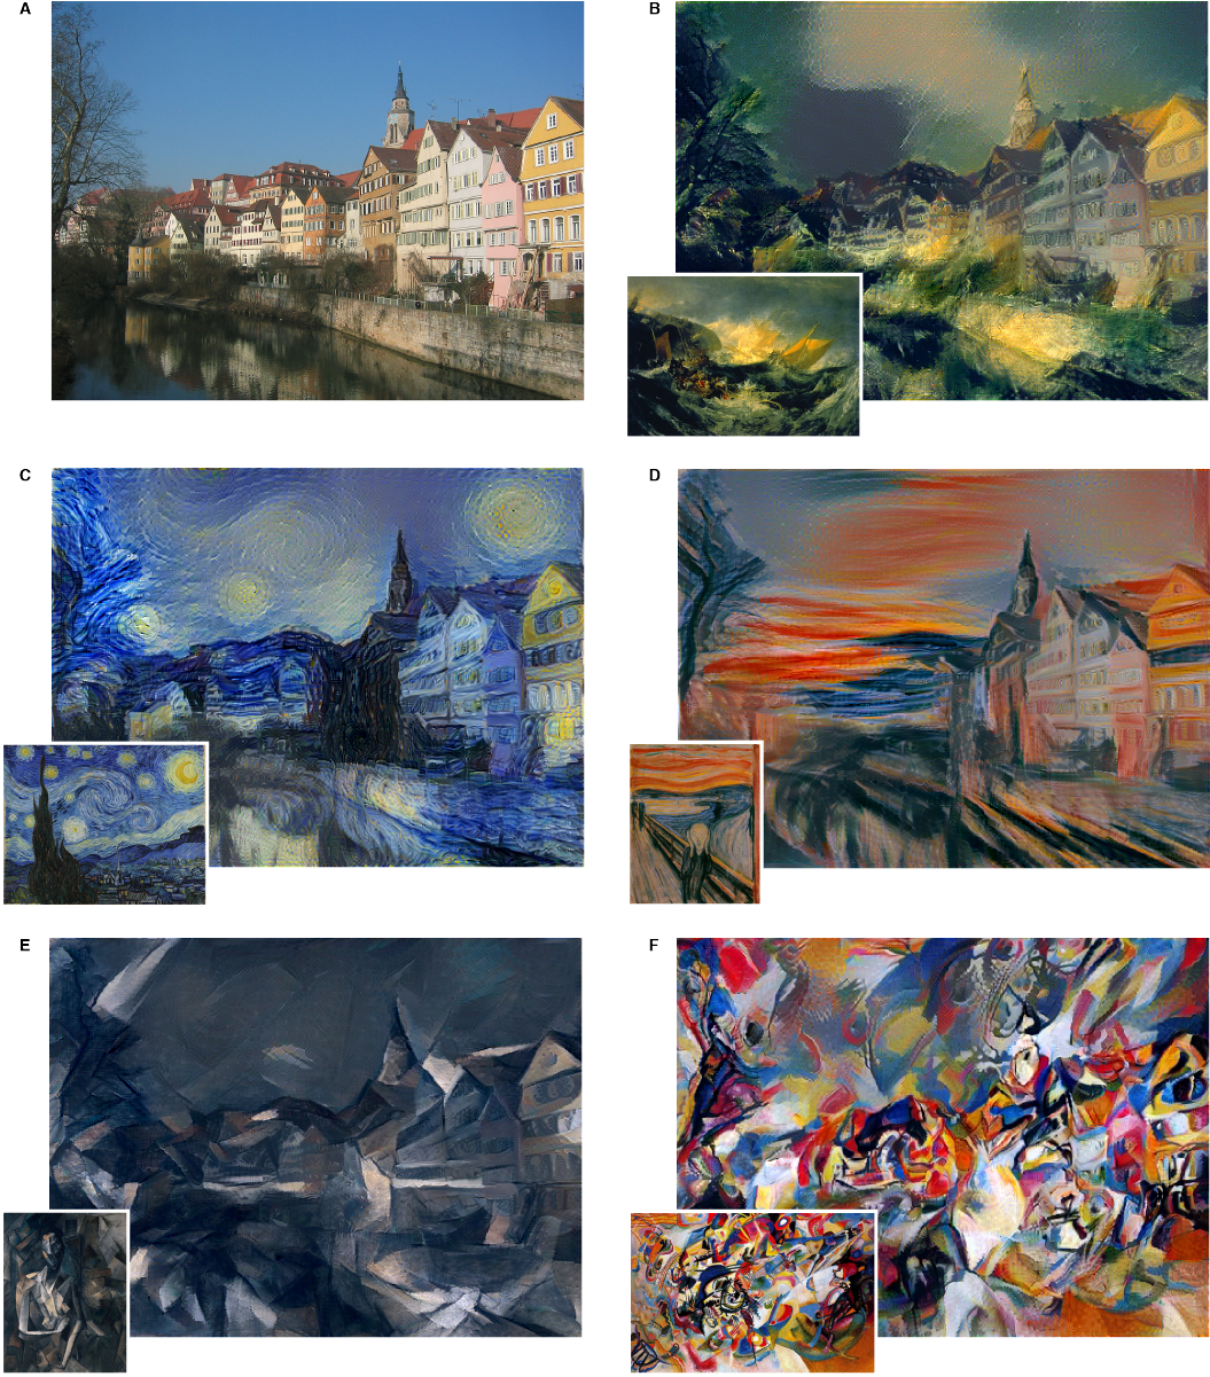
\includegraphics{gatys_ST}
    \caption[]{Style transfer examples by \citeauthor*{gatys}. \cite{gatys}}
    \labfig{content_style_loss}
\end{marginfigure}

The result of this can be seen in \reffig{gatys_ST}

\subsubsection{Follow-Up Research}
There has been some follow-up research on \citeauthor*{gatys}'s work which addresses mainly how the style loss works.

\citeauthor*{MMD} have shown that the style loss is equivalent to calculating the \textbf{maximum mean discrepancy (MMD)} between the features of each layer \cite{MMD}.
MMD is a test-statistic for a null hypothesis $p=q$ with the data $X = \{x_i\}^n_{i=1}$, sampled from $p$, and $Y = \{y_i\}^n_{i=1}$, sampled from q, at hand.
It can be used as a difference measure as well and vanishes only if $p=q$.
\begin{align}
    \text{MMD}^2[X, Y] & = \frac{1}{n^2} \sum^n_{i=1} \sum^n_{i'=1} k(\vec{x}_i, \vec{x}_{i'}) \\
    & + \frac{1}{m^2} \sum^m_{j=1} \sum^m_{j'=1} k(\vec{y}_j, \vec{y}_{j'}) \\
    & - \frac{2}{nm} \sum^n_{i=1} \sum^m_{j=1} k(\vec{x}_i, \vec{y}_{j})
\end{align}

MMD can be based on different kernel functions $k$ and \citeauthor*{MMD} have shown that the style loss is equivalent to the squared MMD with a polynomial kernel.
Consequently they were able to show, that style transfer work with different kernel functions as well and even by explicitly matching the batch statistics (see \reffig{MMD}):
\begin{align}
    d_{\text{style}}^l(\vec{x}, \vec{y}) & = \frac{1}{N_l} \sum_{i = 1}^{N_l} \left( (\mu^i_{F(\vec{x})^l} - \mu^i_{F(\vec{y})^l}) + (\sigma^i_{F(\vec{x})^l} - \sigma^i_{F(\vec{y})^l}) \right)
\end{align}

\begin{figure}
    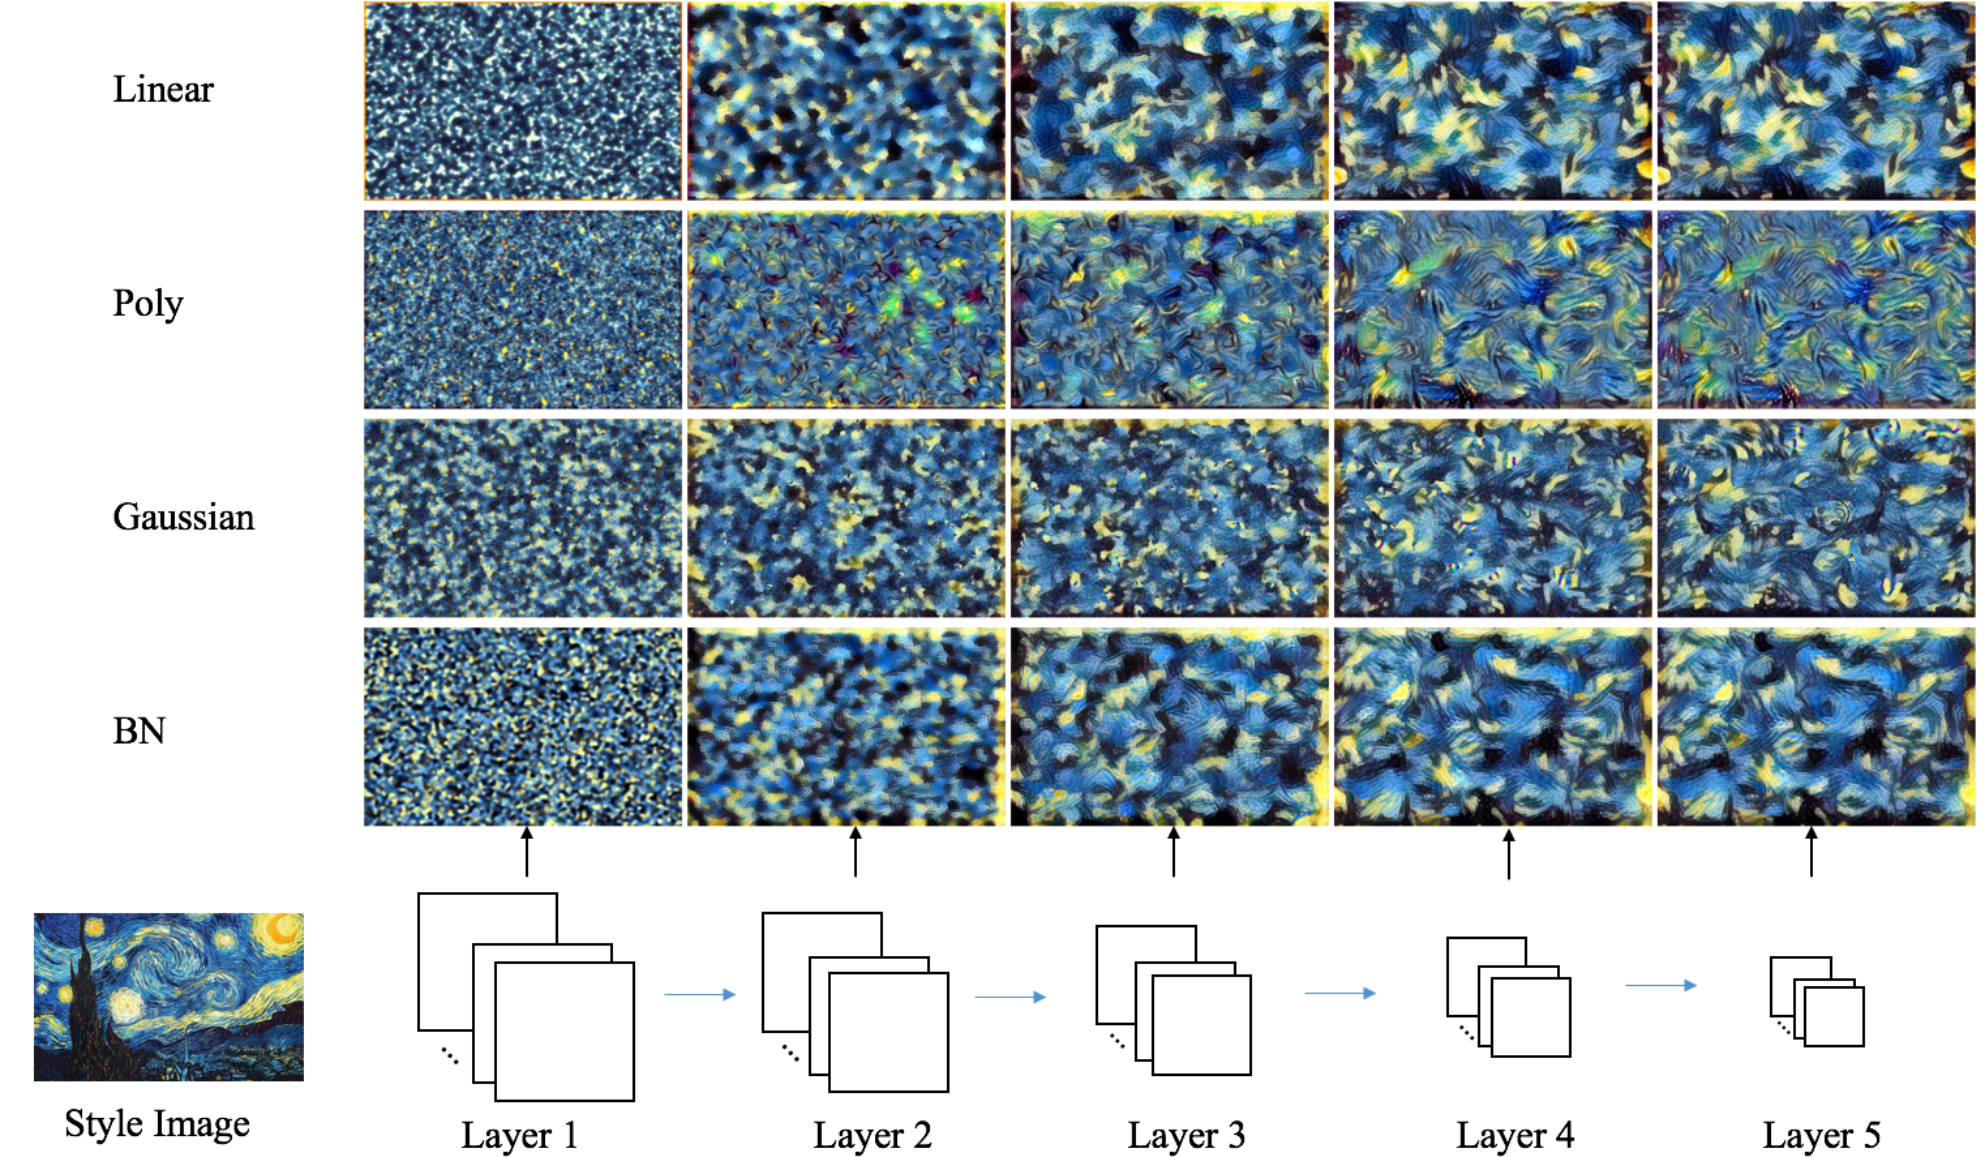
\includegraphics{MMD}
    \caption[]{Reconstructed textures for Starry Night using different kernel functions $k$ \cite{MMD}}
    \labfig{MMD}
\end{figure}


\citeauthor*{LenDu} tested whether pre-trained weights play an important role when performing style transfer.
He was able to show basic style transfer even with random initialized networks, but results vary wisely depending on the random initialization.
Ultimately, it is possible so obtain some style transfer with this technique but the pre-trained weights seem to play an important role in stablizing the reconstruction process.

\subsection{State of the Art}

\subsubsection{Real-Time Style Transfer}
%johnson
Following \citeauthor*{gatys} seminal work, other have followed suit in trying to stylize images with neural networks.
\citeauthor*{Johnson} were the first to use the same losses but train a feed-forward architecture with it \cite{johnson}.
They were able to significantly speed up the stylization process like this as stylization was performed in a single feed-forward pass instead of a lengthy gradient descent optimization.
Ultimately, this enabled them to generate stylized images in real-time from a given content image, using a deep residual convolutional neural network.
\begin{figure*}
    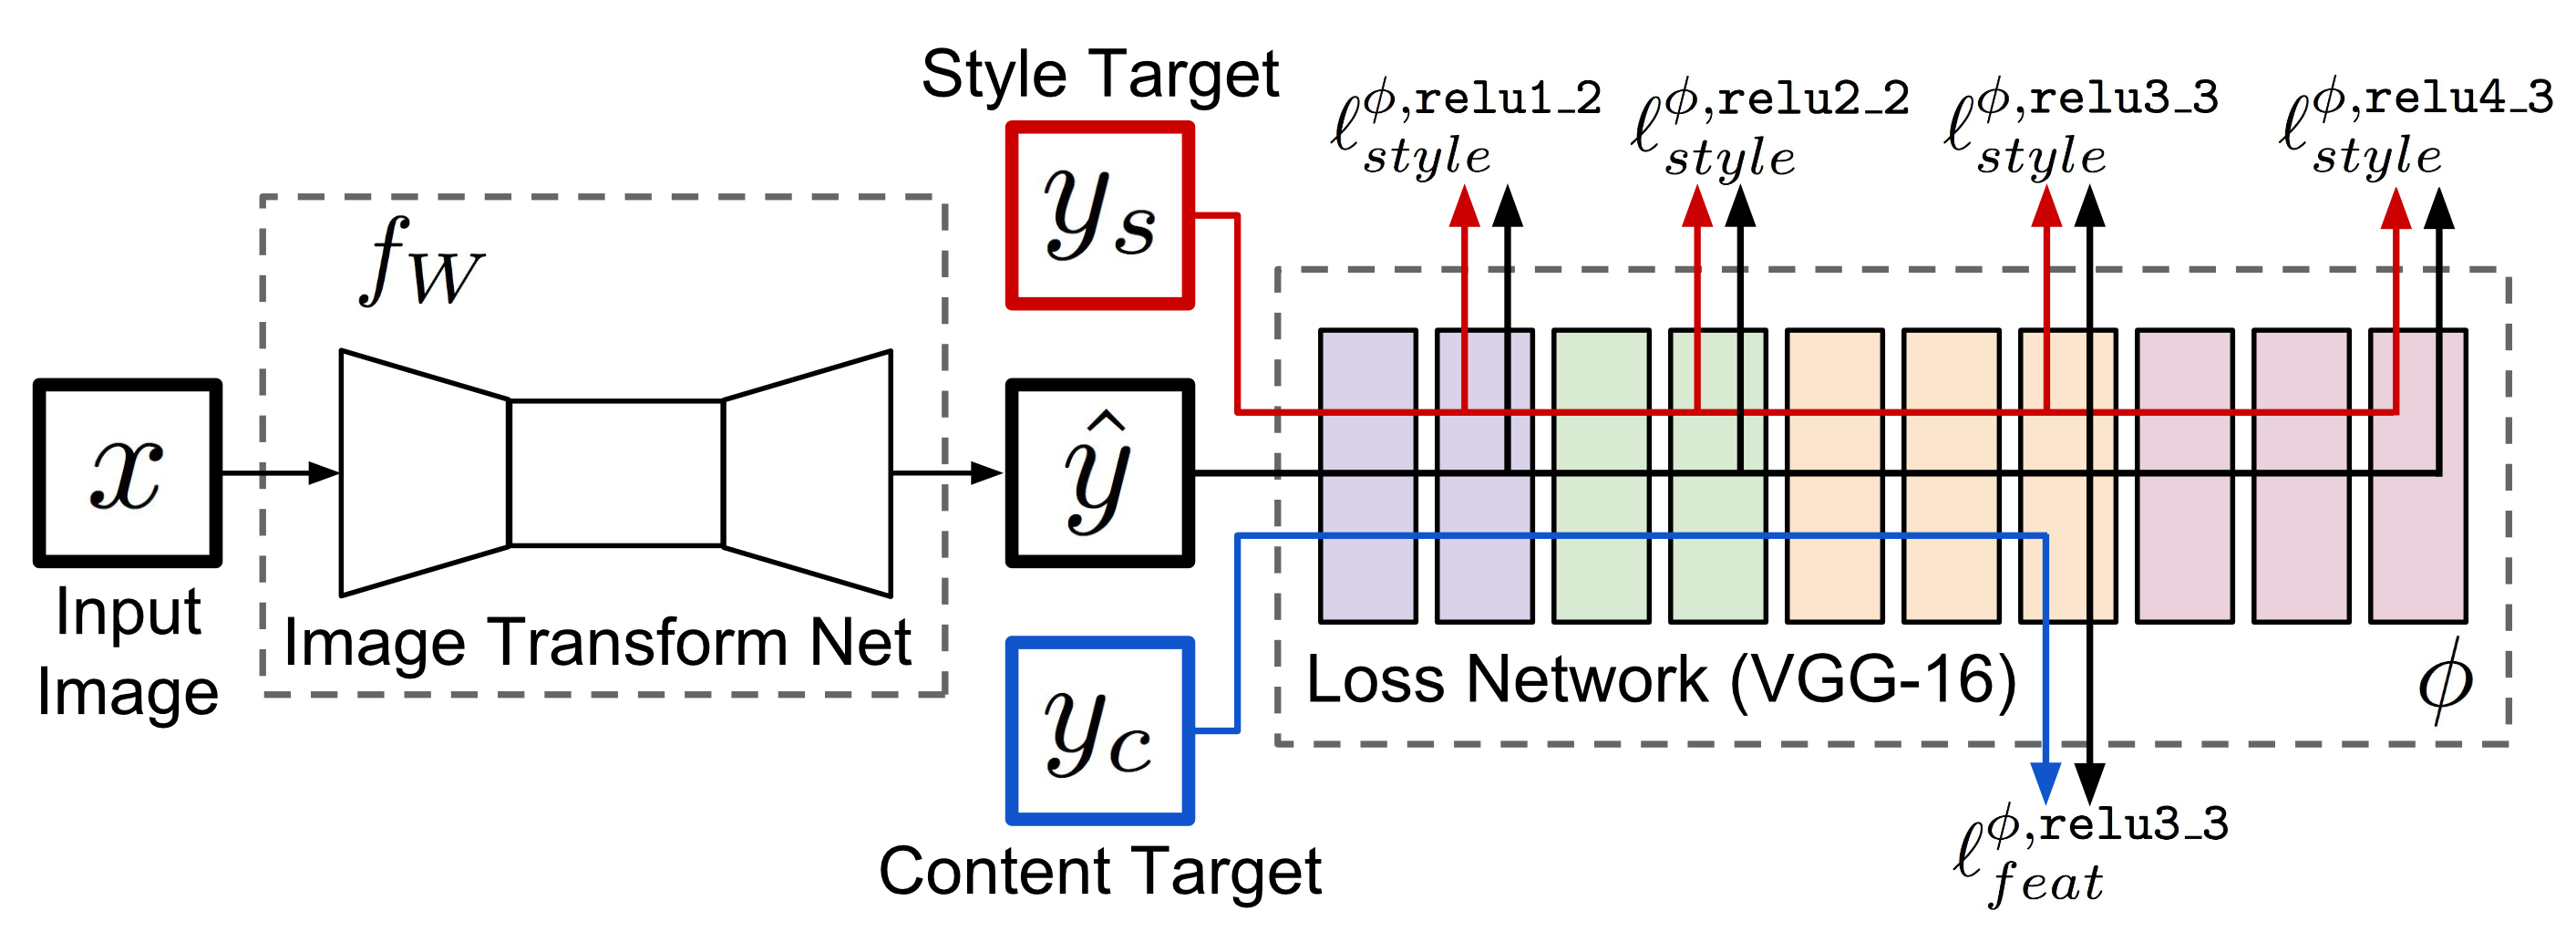
\includegraphics{johnson_net}
    \caption[]{Training set-up by \citeauthor*{johnson}. \cite{johnson}}
    \labfig{johnson_net}
\end{figure*}

%markov random field ansatz?

%adain
\subsubsection{Arbitrary \& Universal Style Transfer}
\citeauthor*{AdaIN} used a different feed-forward approach for arbitrary style.
They first encode an arbitrary style image $\vec{s}$ as well as a content image $\vec{c}$ using a pre-trained VGG network.
This allows them to obtain the activations at a very deep layer of the network $F^l(\vec{s})$ and $F^l(\vec{c})$.
Then they compute the second order statistics for both $\mu_F^l(\vec{s}), \sigma_F^l(\vec{s})$ and $\mu_F^l(\vec{c}), \sigma_F^l(\vec{c})$.
Using adaptive instance normalization (AdaIN), they rescale the content activations such that they match the statistics of the style activations.
\begin{align}
    F'^l = \sigma_F^l(\vec{s}) \frac{F^l(\vec{c} - \mu_F^l(\vec{c})}{\sigma_F^l(\vec{c})} + \mu_F^l(\vec{s}) 
\end{align}
Finally, they train a decoder that minimizes the style and content loss, as they have been proposed by \citeauthor*{gatys}.
They achieve comparable results to other style transfer approaches at a similar speed to \citeauthor*{johnson} while allowing for any target style eventhough only training only once.
\begin{figure*}
    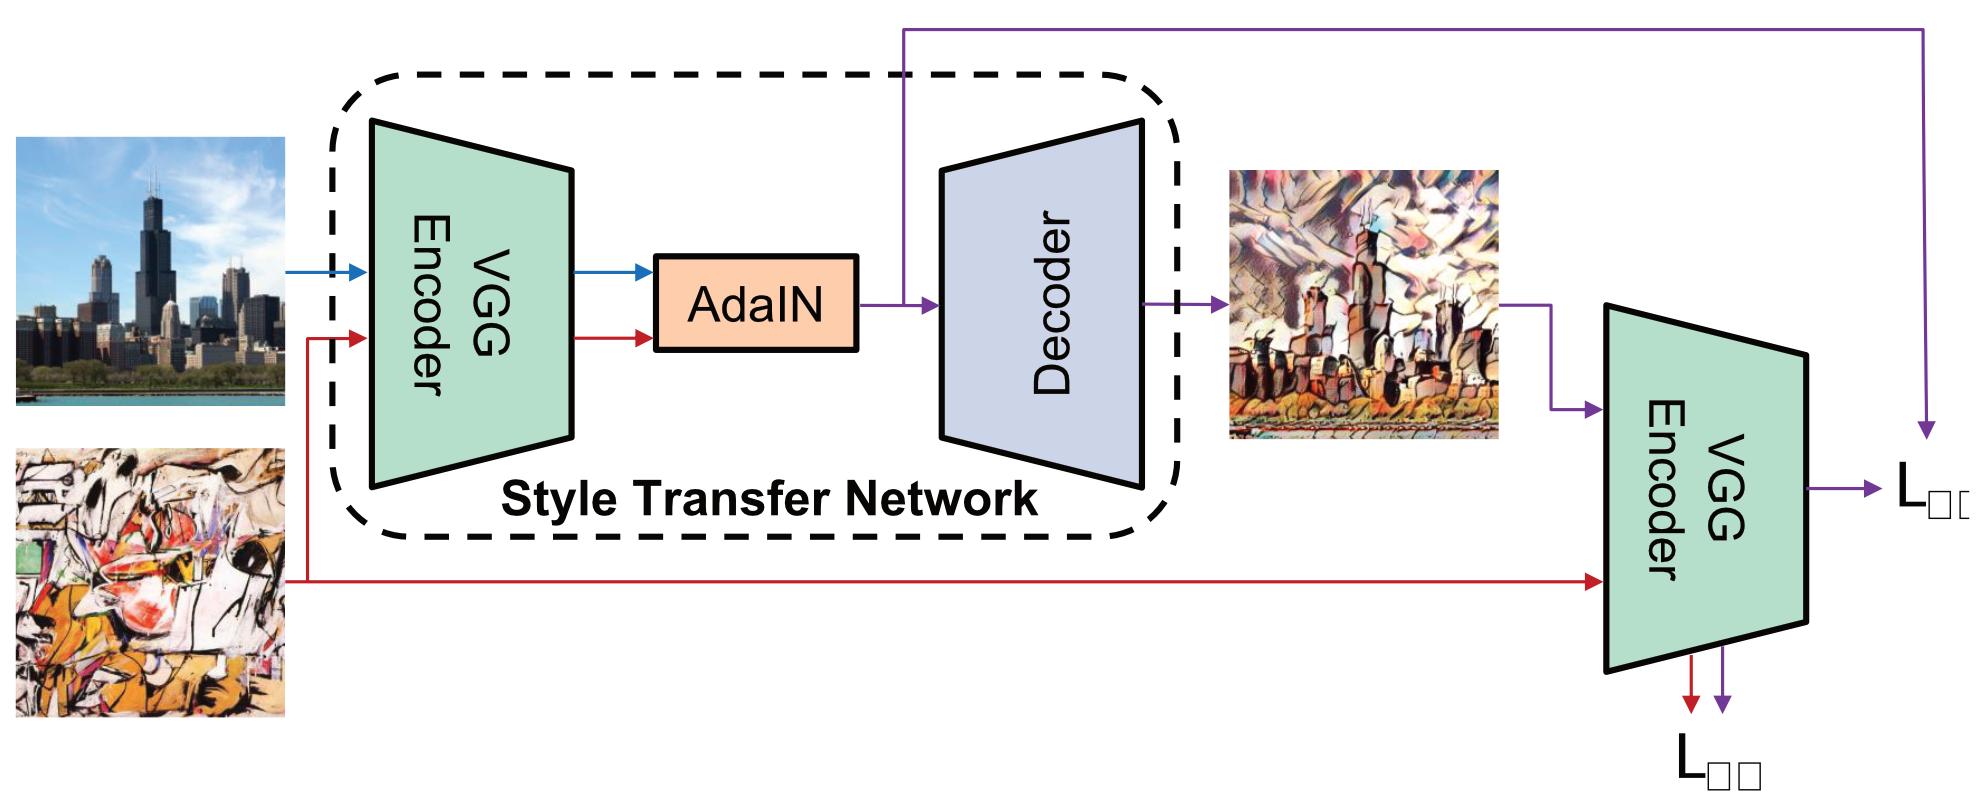
\includegraphics{adain_net}
    \caption[]{Training set-up by \citeauthor*{AdaIN}. \cite{AdaIN}}
    \labfig{johnson_net}
\end{figure*}

%wct
\todo{this is actually just PCA decompsition to a certain degree}
A similar approach by \citeauthor*{WCT} relies on matching the covariance and the mean of content and style activations.
They do that through what they call 'whitening and coloring transform' \cite{WCT}.
First they whiten $F^l(\vec{c})$ into $\hat{F}^l$ such that $\hat{F}^l \hat{F}^l{}^T = I$
\begin{align}
    \hat{F}^l = E_c D_c^{-\frac{1}{2}} E_c^T (F^l(\vec{c}) - \mu_c)
\end{align}
Where $D_c$ is the diagonal matrix of eigenvalues of the covariance matrix and $E_c$ is the respective orthogonal matrix of eigenvectors.
such that
\begin{align}
    F^l(\vec{c}) F^l(\vec{c})^T = E_c D_c E_c^T
\end{align}

Then coloring is performed by rescaling the whitened representation $\hat{F}^l$ into $\tilde{F}^l$
\begin{align}
    \tilde{F}^l = E_s D_s^{\frac{1}{2}} E_s^T \hat{F}^l + \mu_s \\
    F^l(\vec{s}) F^l(\vec{s})^T = E_s D_s E_s^T
\end{align}

The resulting $\tilde{F}^l$ is then decoded with a pre-trained decoder to render the final stylized result.
\citeauthor*{WCT} use pre-train the decoder solely on natural images and perceptual loss and reconstruction loss as objective.
Additionally, they introduce a pipeline that performs style transfer on multiple scales sequentially.
They achieve good results in real-time with just training the decoder once.

\subsubsection{Bidirectional Style Transfer}
%cyclegan
\citeauthor*{CycleGAN} went a different way on style transfer and rely on a generative adversarial objective to identify style in an image.
Specifically, they transform images between any two domains $x \in \mathcal{X}$ and $y \in mathcal{Y}$, not just photos and artworks.
For this, they use two discriminators ($D_X$ and $D_Y$, one for each domain) as well as two transformation networks ($G: X \rightarrow Y$ and $H: Y \rightarrow X$).
Each translation network then transforms a given sample from one domain into the other and the discriminator assesses the result.

\begin{align}
    \L_{\text{adv}} = \log D_Y(y) + \log(1 - D_Y(G(x)))
\end{align}

Additionally, the transformed image is then transformed \textit{again} and compared to the original input, in what they call \textbf{cycle loss}.

\begin{align}
    \L_{\text{cycle}} = \norm{F(G(x)) - x}^2_2
\end{align}

In the end, \citeauthor*{CycleGAN} are able to stylize and de-stylize images with their networks $G$ and $H$.
The main novelty here though is the good stylization quality they achieve without any of the previously introduces style losses.
They have also shown one way, in which GANs are also capable of performing style transfer reasonably well.
Other notable efforts were \todo{list GAN-based style transfer efforts}.

\subsubsection{Adversarial Style Transfer}
Building on these GAN-based approaches, \citeauthor*{artsiom} improved the quality of adversarial style transfer and extended it to abstract styles as well.
They argue that ImageNet-based approaches inherently favor photorealistic styles through the data set that ImageNet has been trained on \cite{artsiom}.
Furthermore, approaches like cycleGAN suffer a similar fate as the back-transformation with cycle consistency opposes loss of detail in more abstract styles.

In order to retain content and global structure of an image, they introduce a fixed-point loss, which requires the stylized image to stay as-is when being re-stylized.
\begin{align}
    \L_{\text{content}} = \norm{E(G(E(x))) - E(x)}^2_2
\end{align}
To minimize this loss, the encoder must understand original content and stylized content.
They also implement a transformed reconstruction loss for better visual quality of the stylized image
\begin{align}
    \L_{\text{transformed}} = \norm{T(x) - T(G(E(x)))}^2_2
\end{align}
The results show good visual quality, especially concerning the details and loss of details for abstract styles.
Also this approach focusses on stylizing not only for a single image but the style of an artist in general.

\citeauthor*{dima} take this further and focus on stylizing different content specifically.
This means, a person is differently depicted than a tree, considering level of detail, colorscheme \etc. , which holds with real-world experience.
They achieve this by using the same fixed-point loss that \citeauthor*{artsiom} but combine it with a second update step.
In this second update step they require similar scenes to be placed closely in feature space and dissimilar scene to lie further apart.
They add a transformation block between encoder and decoder shape the feature space accordingly.

\subsubsection{Others}
There exist many other approaches that are capable of transferring style.
Some focus very heavily on stylization of portraits using self-attention modules \cite{ugatit}.
Others choose an approach similar to cycleGAN but add a shared encoding space for content and separate attribute spaces where style is encoded \cite{unit, munit, drit, drit++}.
With the latter ones mainly focussing on separating shape and appearance of images and recombining them arbitrarily.
One such example is taking the posture of a person in one image and combining it with the clothes and appearance of a person in another image.

The lines between these the applications and style transfer as it has been presented are blurry with many approaches that are capable of performing both.



%\setchapterpreamble[u]{\margintoc}
\chapter{Optimization \& Gradient Descent}
\labch{Optim}

Optimzers have played a very important role for the development of neural networks and their comeback after the so-called 'AI winter'.

The very early implementations of networks like the perceptron, had very straight forward rules for tuning the weights within the network.

These networks were inspired by nature and so was training them.
In accordance to observations made on neurons, weights were 
%what fires together wires together (Hebb's rule)

\section{Optimization Problems}
%optimization
%lagrangian for SVM

\section{Gradient Descent}
%hwo does gradient descent work?

\section{Backpropagation}
%backpropagation finally allowed to train neural networks efficiently

%forward pass
%reverse pass
%gradient descent step
%vanishing gradient problem

\section{Optimization Algorithms}
\subsection{Momentum}
\subsection{Stochastic Gradient Descent}
\subsection{AdaM}
\subsection{Other Algorithms}


%
%\pagelayout{wide} % No margins
%\addpart{Contribution and Experiments}
%\pagelayout{margin} % Restore margins
%
%%\input{chapters/NeuralRenderer.tex}
%%\setchapterpreamble[u]{\margintoc}
\chapter{Stroke Approximation}
\labch{StrokeApprox}

%\input{chapters/Approach.tex}
%\setchapterpreamble[u]{\margintoc}
\chapter{Ablation Experiments}
\labch{Ablations}

%
%\pagelayout{wide} % No margins
%\addpart{Conclusion}
%\pagelayout{margin} % Restore margins
%
%\setchapterpreamble[u]{\margintoc}
\chapter{Discussion}
\labch{Discussion}

This thesis's original goal was to come up with a feed-forward architecture, which can predict brushstrokes in a painting.
This architecture should be built around a differentiable renderer, which renders brushstrokes from parameters.
Such an approach would have two use-cases:
\begin{enumerate}
    \item Generate 'brushstroke representations' of input paintings, which describes paintings as brushstrokes instead of pixels.
    \item Render images as paintings if the input is a photograph.
\end{enumerate}

Especially the aspiration of achieving this with a single feed-forward approach has been proven difficult.
For once, existing approaches either restrict themselves to very low image resolutions or iteratively predict brushstrokes.
As both these compromises ought to be avoided, an orthogonal approach has been chosen.
This approach places many brushstrokes on a virtual canvas.
Then the brushstroke parameters are iteratively optimized through backpropagation.
It was possible to show that a target image with a resolution of $\approx 1$ megapixel can be approximated with such a set-up.

Nevertheless, this approach features some weaknesses.
First of all, it takes approximately one hour per image to obtain a brushstroke representation.
Then, the approach struggles with large uniformly colored regions in images.
The best approximations could be gathered if single brushstrokes are visible and set themselves apart from the background.
Furthermore, the optimization requires many constraints, and lots of compromises are necessary to keep the computational burden low.
The limited data set with only a single control-point, which was used to train the renderer, is a good example of this.

Still, the results could be compared to what others have previously achieved.
The closest approaches to this thesis are those by \citeauthor*{LpaintB} and \citeauthor*{neuralpainters}.\\
\citeauthor*{LpaintB} were able to recreate a painting by sliding a window over it for which brushstrokes are predicted in a feed-forward manner.
The network is trained explicitly for a single image and shows style transfer-like behavior if applied to other images.
It takes about an hour to train the network per 1 MP image, as the author claim.\\
\citeauthor*{neuralpainters} focused his work on training a recurrent approach to predict brushstrokes.
However, he showed a first approach which recreated content in an image by optimizing the brushstroke parameters directly.\\
Both approaches presented a differentiable renderer as a key-element, much like this thesis.

Compared to both of these approaches, this thesis put more effort into building a suitable renderer.
It seems to have paid off when looking at the details in the image.
Brushstrokes show fading and narrowing towards their ends which lines up with real-world observations.\\
When rendering images of van Gogh paintings, it seems as if a majority of brushstrokes aligns with the 'flow' of the original painting.
Especially brushstrokes in 'The Starry Night would follow the curly flow, which can be seen in the original.
Compared to \citeauthor*{LpaintB} the visual quality seems to have improved while a similar amount of time is necessary to approximate a single painting.\\
When considering the stylization of photos, this thesis could only offer a single oil painting-like style.
\citeauthor*{LpaintB} offer more styles (\eg watercolor).
Comparing stylizations is highly subjective.
Thus, readers are encouraged to look at the provided stylizations of the same image and build their verdict (see \reffig{final_stylization}).
A noteworthy aspect is how well this thesis' approach aligns brushstrokes with edges in the stylization, much like artists presumably would choose to do.

\citeauthor*{neuralpainters} presented a stylization approach very close to the approach of this thesis.
Arguably, it comes up with a very nice level of abstraction.
As this thesis focused harder on being closer to the original image, these two approaches are hard to compare.
Nonetheless, it would be desirable to achieve similar levels of abstraction by tweaking the approach of this thesis.


Another comparison has was made to brushstroke extraction.
\citeauthor*{lamberti} presented an approach aimed specifically at extracting brushstroke properties from painting images.
This thesis also aimed at extracting brushstrokes from images.
Up until now, there has not been a known neural network-based approach to do so.
Comparisons showed that \citeauthor*{lamberti} were able to extract single brushstrokes more precisely.
Still, the rendering based approach of this thesis was able to cover the whole image area better.
Also, it seems that this thesis' approach is able to capture group dynamics broadly.
This could be seen as a first step towards accurately parametrizing paintings with a neural network.


%Verdict
Ultimately, it was indeed possible to generate a brushstroke parametrization for images of paintings.
Although it was not possible to achieve this with a feed-forward approach, the subsequent optimization-based approach still fares well against state-of-the-art counter-parts.
It could even be argued that such an optimization-based approach scales easier than other approaches and enables high-resolution image sizes.
The image resolution of up to one megapixel is especially noteworthy and probably a key factor in generating such detailed renderings.
%%goal achieved?
%%nice image resolution

Surprisingly, the stylization of photographs, which was initially a byproduct of the approach, gave relatively good results.
It could be argued that it is comparable in quality to the best approaches as of mid-2020.
%%is probably a state of the art painterly rendering approach in terms of quality
The other actual goal of generating accurate brushstroke representations of images has not been quite so successful.
The comparison to brushstroke extraction algorithms showed that brushstrokes are not captured as accurately as hoped.
Especially when comparing the details to the original paintings, it becomes evident that the rendered brushstrokes still look significantly different.
Thus the results seem relatively appealing from afar, but less so when getting closer.

It raises the question of whether the extensive work that went into the renderer was worth it.
It seems that the goal of generating real-looking brushstrokes may clash with having a versatile and more efficient renderer.
Future approaches should definitely ask whether the renderer should focus even more on realism or rather tend towards a more simplistic approach. 
%was it worth putting that much effort into the renderer?
This is maybe also a question which could have been dealt with in the course of this thesis.
Other ways could have been thought of, how brushstrokes are parameterized, and it would have been interesting which differences it had made.
%more testing with regard to the brushstrokes could have been performed
%Other approaches to the brushstroke renderer, use paths instead of predefined and paired samples

Another aspect would have been testing different optimizers (\eg L-BGFS) besides the standard AdaM-optimizer.
%different optimizers should have been tested (L-BGFS)

At last, the question arises whether this work will be relevant for the future.
As artistic style transfer is more of a niche than a mainstream field in computer vision, it seems at first as if there is little relevance in this work.
Nevertheless, it was possible to show that state-of-the-art results in painterly rendering can be achieved by employing an approach that could be called dated.
Also, it is imaginable that the resulting brushstroke parametrization could be used for other purposes, such as style transfer on a brushstroke level.
%Is this something that will be used in the future? / relevance?
% parametrized representation is interesting for GNNs and other emerging techniques.
Other possible improvements and future ideas based on this thesis will be explained in the next chapter.

All-in-all, the results are two-faced.
Stylization works reasonably well, but parametrizing paintings leaves much to wish for.
Still, the approach and its results could be seen as a proof-of-concept for simple optimization-based approximation.


%\setchapterpreamble[u]{\margintoc}
\chapter{Outlook}
\labch{Outlook}

%
%\appendix % From here onwards, chapters are numbered with letters, as is the appendix convention
%
%\pagelayout{wide} % No margins
%\addpart{Appendix}
%\pagelayout{margin} % Restore margins
%
%\input{chapters/Appendix.tex}

\include{chapters/Introduction}

\pagelayout{wide} % No margins
\addpart{Theoretical Background \& Related Work}
\pagelayout{margin} % Restore margins

\setchapterpreamble[u]{\margintoc}
\chapter{Machine Learning \& Computer Vision}
\labch{MLandCV}
In this chapter the theoretical backgrounds and motivation of Neural Networks ought to be explored.

First, a physical/biological motivation will set the foundation for the theoretical background accompanied by a more mathematical motivation.
Thereafter, more advanced lines of thought will be introduced that finally lead to convolutional neural networks as the current driving force in computer vision .

\section[Artificial NNs]{Artificial Neural Networks}

\subsection[Inspiration]{Neurobiological Inspiration}

%Nature is often inspiration (birds and planes)
Many human achievements have at least been partially inspired by studying nature.
A very popular example is that of airplanes and birds.
The study of how birds are able to fly found that the shape of their wing is the essential element to flying.
Inventors and engineers have taken this inspiration and slowly but steadily created planes and the like from it.
%arguabnly implementations deviate from nature (plane and bird) and people say to refrain from using these analogies.
Yet, planes are not birds, as they are not flapping their wings (yet?), but integrate of other inventions like jet engines to get the same (or better) capability of flying as birds.

Quite similarly, the brain features a lot of insights, how intelligence or something that seems like it, can be constructed.
In the same way humans studied birds to understand flying, researchers are now studying the brain to create better artificial intelligence.

In the earliest stages of this they would try to imitate the brain, as people have tried imitating birds at first and failed similarly.
\begin{figure}
    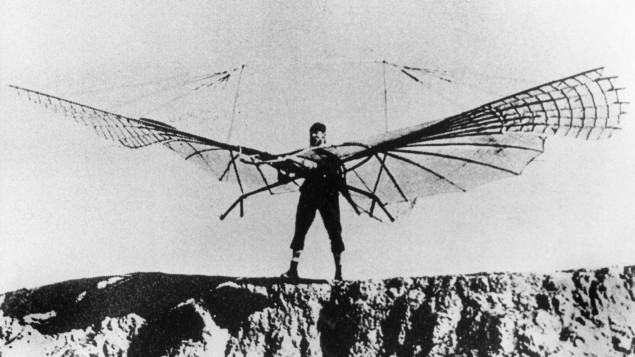
\includegraphics{otto_lilienthal}
    \caption[]{Otto Lilienthal with his flying apparatus. \url{https://www.deutschlandfunkkultur.de/geschichte-der-fliegerei-wie-der-mensch-die-voegel.976.de.html?dram:article_id=308043}}
    \labfig{lilienthal}
\end{figure}
\marginnote{There is current research on replicating the brains structure to the neuron level on hardware with more success \cite{brainscales}.}

%start with a very much simplified model McCulloch and Pitts
%binary input and binary output
Warren McCulloch and Walter Pitts proposed one of the earliest models of a neuron, which targeted simplifying the real Neuron.
\marginnote{Notably McCulloch and Pitts (1943) even preceded Hodkins and Huxley's (1952) Nobel price winning description of a neuron.}

%explain biological neuron
\subsubsection{Biological Neuron}
For this the functioning of a neuron shall be described shortly.

Human cells in that make up the brain are called \textbf{neurons}.
They connected to each other through dendrites, synapses and axons and they use these connections to send signals.

A neuron receives signals through its dendrites, which all lead to the cell body (soma).
At the cell body the signals are accumulated.
If the summed value of the signals' potential reaches a certain threshold, an action potential is generated.
The new signal then travels along the axon and its branches towards other neurons.
The axon ends in synapses which connect the axon to other neurons' dendrites.
Synaptic transmissions are usually mediated by chemicals and not by electrical signals.
The chemical nature of the synapse allows it to forward either an excitatory or an inhibitory signal.
Excitatory signals will bring the cell potential closer to the threshold, while inhibitory do the opposite \cite[p.~42]{coloratlas}.
\marginnote{Cell potentials are usually decreases by excitatory signals, as the action threshold sits below the resting potential.}

What makes the brain so powerful though, is not the neuron itself with its arguably simple structure but the vast network of billions of these neurons.
Each neuron is connected to thousands of other neurons with which it constantly communicates.
How a signal is transported between the neurons depends on the interplay of synaptic weights, neuron connections and the threshold of each neurons.

\subsubsection{Artificial Neuron}
McCulloch and Pitts saw that powerful things can be achieved when connecting lots and lots of simple structures.
Thus, they proposed an even simpler model of a neuron:

They restricted their neuron to a binary state (on or off).
Each neuron then has a number of incoming signals from other neurons which would either be positive or negative.
A neuron would only become active if the number of incoming positive signals minus the number of negative signals exceeds the neuron's threshold.
\todo{add equation with activation function, when neuron fires}
McCulloch and Pitts then also changed the highly parallel and complex nature of biological neural networks to a single layer feed-forward network architecture.

In a feed-forward network neurons are grouped into layers and operate in parallel within a layer.
Each neuron in a layer is fed the same input signal (often described as an input layer).
The neuron's state is then computed according to an equation such as \refeq{mcculloch}.
The activation value of each neuron then defines an output.

As this models deviates from nature quite a bit, these structures a better referred to as \textbf{units} instead of neurons.

In a single layer architecture a layer often consists of a single unit (see \reffig{ff_arch}.
Basically, input signals come from one side and output signal go out the other side, which can be expressed in a simple equation like \refeq{mcculloch}.
This is not only done for practical reasons but also inspired by observation of layered neuron structures in the brain.

The McCulloch-Pitts model is capable of emulating simple logical relations (|AND|, |OR|, |NOT|) but nor |XOR| which will be explained later.

\subsubsection{Perceptron}
This McCulloch's and Pitts' is very much simplified yet comes with some weaknesses.
Thus, the \textbf{perceptron} has been introduced by Frank Rosenblatt in 1957.
Instead of having a binary unit, he came up with a linear threshold unit (LTU).
The LTU allows for numeric instead of binary signals which can be weighted with independent factors.
Also they use the 'bias trick' to parametrize the threshold or bias of the unit as yet another weight for an input that is constantly one.
The resulting equation for each LTU then reads:
\todo{equation for LTU with bias trick}
Equation \refeq{LTU} can then be formulated in a vectorized form such that:
\todo{vectorized LTU}

In this form the calculations for each unit become mathematically and computationally relatively easy.
Each layer can be expressed as a vector of activations $\vec{x}$.
Multiplying this vector with the weight matrix $\mat{W}$ and applying the element-wise activation function returns the activations for the subsequent layer.
\marginnote{The word perceptron describes the whole function $f$ in equation \refeq{perceptron} which can consist of many LTUs}
%simplified computational model of how biological neurons might work together
This simple yet capable description of a unit built the base for a first surge of interest in neural networks.
%connectionism

\subsubsection{Mathematical Interpretation}
%hyperplane
%linear separation
%bias trick
The very simplistic mathematical formulation of the perceptron suggests that there might be a mathematical meaning to it besides the biological analogy.
Indeed, the perceptron is equal to the definition of a \textbf{binary linear classifier}.

A binary linear classifier, classifies inputs into two classes, hence binary.
It does so by drawing a virtual hyperplane in input space and predicts the class for each input, depending on whether it lies above or below this hyperplane.
\begin{marginfigure}
    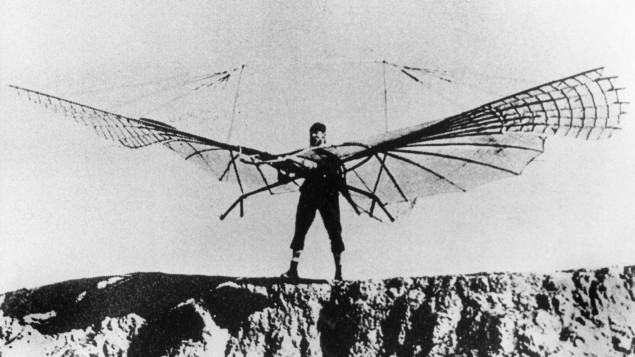
\includegraphics{otto_lilienthal}
    \caption[]{As a very simple example, this binary classifier has data on how often the words 'weightloss' and 'invest' appear in an email.
Any time these two words appears too often and the data point is above the decision boundary, the email is classified as 'spam'}
    \labfig{linear_class}
\end{marginfigure}
As the hyperplane (or decision boundary) is quantified by a linear function, the classifier is described as linear.

A classic problem would be classifying email as spam.
Given the two data inputs (\ie frequency of of the words 'weight loss' and 'invest') the classifier has to make a decision.
For this reason the binary classifier defines a \textbf{decision boundary}.
Any data point that lies above this decision boundary is classified as 'spam', any point beneath is classified as 'not spam'
This makes sense as normal email rarely use the two words.
For other people like a nutritionist, the word weight-loss can come up more frequently.
This means the decision boundary differs for different users and their mail.

To compute where a point lies relative to the decision boundary, a data point's value along each axis $x_1, x_2$ is weighted individually $w_1, w_2$ and summed with a bias $b$.
The result is checked whether it is above or below a threshold $t$.
\begin{align}
    z = w_1 x_1 + w_2 x_2 + b
\end{align}
With the classification 'spam' if $z > r$ and 'not-spam' $z \leq r$ (\textit{in dubio pro reo}).
Equally $z - r > 0$ holds for spam as well such that the threshold can be brought into the equation and $z$ is checked against $0$.
$r$ can then be absorbed into the bias.
%predistion is y, 1 is spam, 0 is not spam
\begin{align}
    \rightarrow z = w_1 x_1 + \hdots + w_D x_D + b - r = w_1 x_1 + \hdots + w_D x_D + b'
\end{align}

For arbitrary dimensions $D$ this becomes
\begin{align}
    z = w_1 x_1 + \hdots + w_D x_D + b
\end{align}
 where $\vec{x}$ and $\vec{w}$ can be defined by vectors
\begin{align}
    z = w_1 x_1 + \hdots + w_D x_D + b = \vec{w}^T \vec{x} + b
\end{align}
The decision boundary can be easily derived from this, since $\vec{w}$ is the orthogonal vector to the hyperplane and $\frac{b}/\norm{\vec{w}}$ is the displacement of the plane along $\vec{w}$.

For a simpler notation one can define an additional 'virtual' input which has a constant value of $1$ as $x_0$, the bias $b$ can then be elegantly included into $\vec{w}$.
\begin{align}
    z = w_0 b + \vec{w}^T \vec{x} = w_0 b + w_1 x_1 + \hdots + w_D x_D = \vec{\hat{w}}^T \vec{x}
\end{align}
with $x_0 = 1$ and $w_0 = b$.
This is called the \textbf{bias trick}.

This description also holds for perceptrons with more than one unit.
In that case, the input vector $\vec{x}$ and the weights $\vec{w}$ become matrices with multiple column vectors.
\begin{align}
    \vec{x} \rightarrow (\vec{x}_1, \vec{x}_2, ...) = \mat{X}
    \vec{w} \rightarrow (\vec{w}_1, \vec{w}_2, ...) = \mat{W}
    \rightarrow \vec{z} = \mat{\hat{W}}^T \vec{X}
\end{align}
%\todo{take this to high-dim space and explain ability to imitate any linear function.}


\subsubsection{Loss Function}
Now with a mathematical definition at hand the next step is to quantify the output.
In order to train a classifier, an objective has to be formulated though a \textbf{loss function}.
Usually (in the supervised case), there is already data set on which the network can be trained.
In the given example this would be mails which were read beforehand and then declared either 'spam' $\tilde{y}_i = 1$ or 'not-spam' $\tilde{y}_i = -1$
$\tilde{y}_i$ is called the \textbf{label} for a sample $x_i$ with index $i$.

With the binary linear classifier, the decision boundary has been introduced ($z_i > 0$ ?) to predict this label for any given sample.
This is sufficient to predict a class but a lot of information is lost this way.
For training and evaluation the information available in $z$ should be used.
\eg a large $z$ implies that the data point is far away from the decision boundary, thus, the classifier is very sure for this classification.
For $z \approx 0$ the classifier is not that sure and for $z = 0$ the classifier is indecisive.
Ultimately, $z$ can be viewed as a score that is calculated for each data input.

The question then becomes how to quantify how well the classifier performs on the given data.
For this reason a loss function is defined which measures the classifier's performance on the data.
A straight forward choice is \textbf{least squares}, where the score's distance to the label is measured.
\begin{align}
    \L_{\text{LS}} = \sum_i (y_i - z_i)^2
\end{align}
The value of the loss function become minimal for $y_i = z_i$ for $i = 1,...,N$.
Yet, this score function is especially susceptible to outliers which will cause the decision plane to skew towards outliers with $z > 1$ or $z < -1$

For this reason \textbf{support vector machines (SVM)} employ a \textbf{maximum margin} classifier.
A maximum margin classifier seeks to find a decision boundary which as far from the closest representatives of each class as possible (see \reffig{SVM}).
The maximum margin is defined as
\begin{align}
    \text{margin} = d_+ + d_-
\end{align}
with $d_+$ the distance to the nearest training sample with class $+1$ and $d_1$ the closest training sample for class $-1$.
Noticeably, this requires for the data to be linearly separable, which means that there must exist a hyperplane which perfectly separates the data according to its class.
The margin becomes maximal for $d_+ = d_-$.
Since $w$ is orthogonal to the hyperplane, $\vec{w}$ can always be rescaled such that 
\begin{align}
    d_+ = d_- = \frac{1}{\norm{\vec{w}}}
\end{align}

Additionally, $\vec{w}$ can be chosen such that $z = \vec{w}_i^T \vec{x}_i + b_i \geq +1$ for $\tilde{y}_i = +1$ and vice versa for $\tilde{y}_i = -1$.
Thus,
\begin{align}
    \tilde{y}_i z_i \geq 1
\end{align}
will hold, for all $x_i$ with equality for points on the margin, as there is always at least one point on the margin.

Thus,
\begin{align}
    d_- = d_+ = \frac{1}{\norm{\vec{w}}}
\end{align}
and the margin
\begin{align}
    d_- + d_+ = \frac{2}{\norm{\vec{w}}}
\end{align}
is maximized when $\norm{\vec{w}}$ is minimized.

Subsequently, the classification can be expressed as a relatively simple optimization problem.
\begin{align}
    \argmin_{w, b} \frac{1}{2} \norm{\vec{w}}^2
\end{align}
under the constraints
\begin{align}
    \tilde{y}_i z_i = \tilde{y}_i (\vec{w}_i^T \vec{x} + b) \geq 1 \forall i
\end{align}
How to solve this optimization problem shall be explained in \refssec{svmopt}

%\todo{perceptron usually just have a step function as activation for classification}
%What is the goal of training?
%hint at backpropagation but this will come in later.


%loss/score function
%(multiclass) (linear) discriminant function

%classifiers come in many forms, one is an SVM with a linear kernel is identical to a perceptron

%linear regression and linaer svm are identical

%linear binary classification
%find values for weights

%scalability
%neurons is activated if a number of inputs is active
%neurons can also be inhibitant
%focussed on logical computations

%explain the logic from neuron to perceptron

%perceptron invented by Frnak Rosenblatt (linear threshold unit)


%perceptron is one layer of LTUs
%weights shoul dbe reinforced when they lead to the correct output

%algebraic fomralism
%bias trick


\section[Fully Connected NNs]{Fully Connected Neural Networks}
\subsection{Multi-Layer Perceptron}
With the perceptron at hand for which is capable of classification any linear separable data, the question becomes, what are the limitations to this?
Minsky and Pappert found the limitations in 1969 with their book 'Perceptrons'.
They oulined the limitations of perceptrons with the |XOR| problem.
The problem becomes obvious when looking at the |XOR| problem in a 2D plane (see \reffig{XOR})
\begin{marginfigure}
    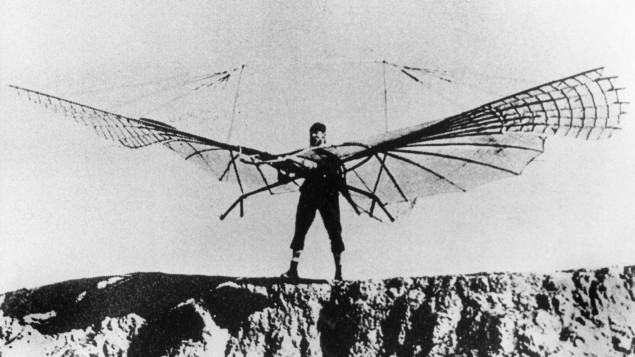
\includegraphics{otto_lilienthal}
    \caption[]{|OR| and |XOR| operations visualized. The |XOR| problem cannot be solved by drawing a single line.}
    \labfig{XOR}
\end{marginfigure}

As it has been explained in the previous section, the perceptron is equal to a binary linear classifier.
As such, the perceptron can only classify linear separable data perfectly.
Since the |XOR| problem can obviously not be solved with a straight line separating the two classes, the perceptron is also not able to compute such an operation. 

This realization led to the first decline in interest in artificial neural networks.

Since then there have been ways of solving this problem for SVMs by projecting the data into a higher dimensional space.
Another approach kept the logic as is but went from the existing shallow network approaches to deep neural networks (DNN).
\textbf{Deep Neural Networks (DNN)} are ANNs which consist of more than one hidden layer.
A single perceptron may not be capable of computing |XOR| but it is capable of calculating |AND|, |OR| and their negated forms.
By using one perceptron with two units to compute |AND| and |OR|, a second layer perceptron can use compute |XOR|
\begin{align}
    XOR(x, y) = AND(OR(x, y), NOT(AND(x, y)))
\end{align}

Now, the |XOR| problem becomes solvable.

\marginnote{The ability to stack multiple layers in ANNs stems from discovery of backpropagation which shall be explained in \refssec{backprop}.}

As before only linear functions could be approximated by perceptrons, multiple layers of perceptrons allow for any higher degree function to be approximated as well.
Thus, \textbf{Multi-Layer Perceptrons (MLP)} sparked new interest in the field of artificial neural networks.

This interest also originated in the similarly layered structure that has been found in the brain.
\begin{marginfigure}
    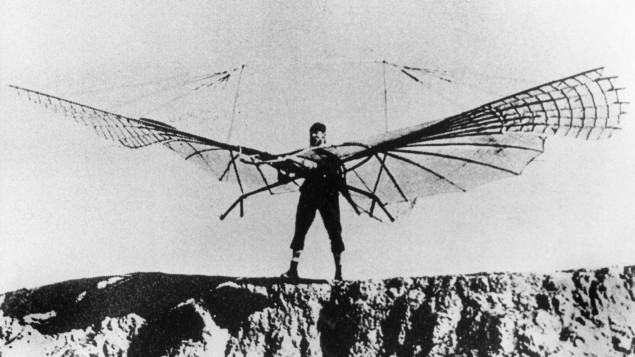
\includegraphics{otto_lilienthal}
    \caption[]{The brains structure under a microscope}
    \labfig{brain}
\end{marginfigure}
\begin{marginfigure}
    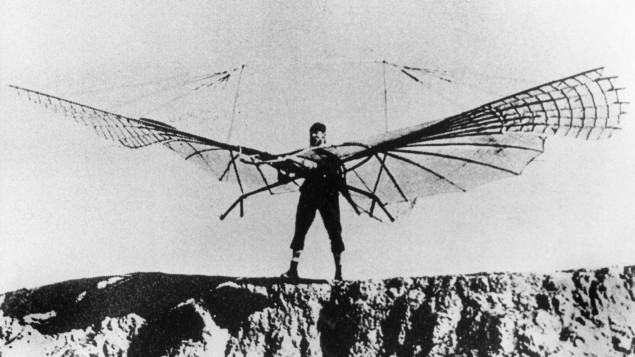
\includegraphics{otto_lilienthal}
    \caption[]{Layers of an MLP}
    \labfig{MLP}
\end{marginfigure}
Ultimately, MLPs really start to show the connected structure in a network that is typically expected.

MLPs are also called \textbf{fully connected networks} since each unit is connected to all unit in the previous layers as well as all units in the next layer.

%\marginnote{This new connectedness opens a realm to a whole field of studies on graphs, networks and network motifs \cite{network_motifs}.}

%histrocal rollercoaster of interest (AI winter) ?
%limited capabilities of the perceptron for XOR problem
%use either higher dimensional input -> kernel trick or stack many perceptrons
%any 2 layer MLP can approximate any continuous function (or somethign like that)
%simialrity to network motifs, make a large network of many identical pieces
%similar to how the brain works as well.

\subsubsection{Activation Functions}
%linear algebra shows that any linear function can approximated by just two perceptron layers for a linear activation function -> more layers do not make sense.
These newfound capabilities for MLPs are not only restricted to binary operations but will translate into continuous space.
In this case the hidden-layer perceptrons get stripped of their activation function.
The activation function of a perceptron has been used up until now to make a class prediction $y$ from the score $z$, which is also called pre-activation.

Replacing the step function with a linear activation function (\ie identity function), each hidden-layer's perceptron would initially seem to increase the capabilities of the MLP.
Unfortunately, this is not the case as any subsequent perceptrons with linear activations can be reduced to a single preceptron.
\begin{align}
    \vec{z}_2 = \mat{w}^T_2 \vec{z}_1(\vec{x}) = \mat{w}^T_2 \mat{w}^T_1 \vec{x} = \mat{w}' \vec{x}
    \labeq{LAF}
\end{align}

Consequently, the step-function that was used in the |XOR| problem played an important role.
The reason for this is the non-linear nature of the step-function in contrast to any linear activation function.
It can easily be shown, that \refeq{LAF} does not hold for non-linear activation functions.

Thus, the question becomes which other activation functions there are that go beyond binary classification.
An early popular choice are sigmoid functions (logistic function or $\tanh$).
Especially the logistic function is popular due to its similarity to the step-function amongst other things.
\begin{align}
    \sigma(z) = \frac{1}{1 + e^{-z}}
\end{align}
\begin{marginfigure}
    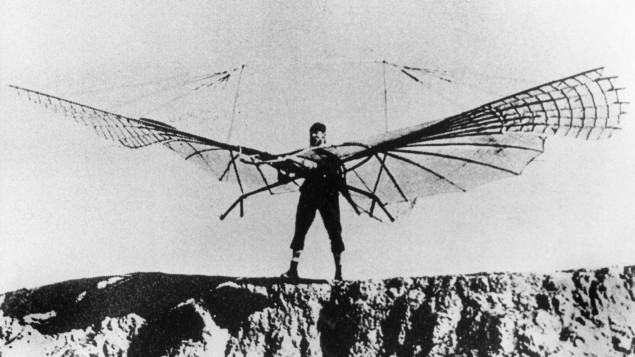
\includegraphics{otto_lilienthal}
    \caption[]{A sigmoid function. It saturates to $1$ for very large inputs and $0$ for very small inputs, similar to the step function.}
    \labfig{sigmoid}
\end{marginfigure}

Another popular choice are rectified linear units (ReLU) which are identical to a linear activation for $z > 0$ but mimic the step function for $z < 0$.
Basically, a ReLU suppresses the signal of a perceptron until it reaches the threshold of $0$ and then forwards the signal unaltered.

Another activation function 'leaky ReLU' attenuates the signal below the threshold with a factor $\alpha$ instead of fully suppressing it.
\begin{marginfigure}
    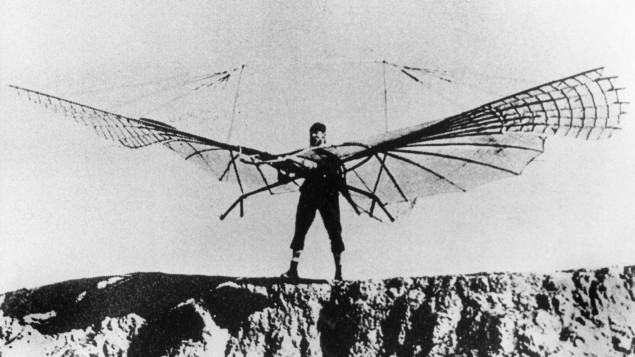
\includegraphics{otto_lilienthal}
    \caption[]{ReLu activation function}
    \labfig{relu}
\end{marginfigure}
\begin{marginfigure}
    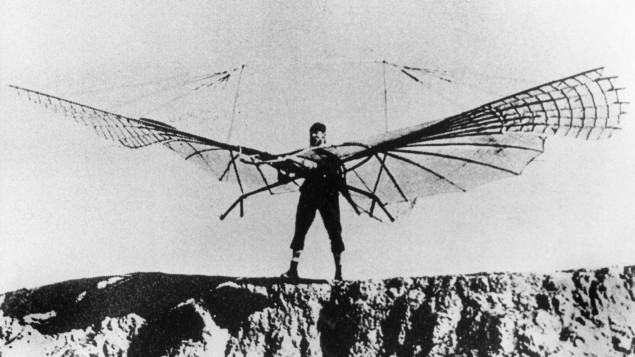
\includegraphics{otto_lilienthal}
    \caption[]{leaky ReLu activation function with $\alpha = 0.2$}
    \labfig{lrelu}
\end{marginfigure}


%move on from step function as activation
%Activation functions have already been used to describe the perceptron and the artificial neuron by McCulloch and Pitts.
%In both cases (as well as the binary linear classifier) the inputs are weighted and summed up to something called a \textbf{pre-activation} \cite[p.~6]{GrosseNotes}.
%The pre-activation is then checked against a threshold which is often $0$ if there is a bias term involved.
%In all previously given cases this decides whether a unit becomes active or which class the input is allocated to.
%\begin{align}
%    \sigma(z) = \frac{1}{1 + e^{-z}}
%\end{align}
%
%There are many more activation functions with different properties such as the \textbf{sigmoid activation} $\sigma$.
%\begin{align}
%    \sigma(z) = \frac{1}{1 + e^{-z}}
%\end{align}
%$\sigma$ is also inspired by nature as a neuron can fire at different rates according to its input.
%Even though this is very much simplified, the main idea is, that a strong input ('mentioning 'weightloss' hundreds of times) should lead to a strong output ('this mail is definitley spam').
%
%\reffig{sigmoid} shows that the output $\sigma(z)$ scales with the input $z$ but saturates for both very large and very small $z$.


%inability to solve XOR problem
%thus stack multiple 
%non-linearity is important 

%hiddenlayers

%After motivating the perceptron, this section will focus on combining multiple layers of perceptrons, which make up the \textbf{multi layer perceptron (MLP)}.
%The MLP combines several perceptron layers in series which is the first step towards what is described as deep neural networks.
%In a first thought experiment the original input layer and the output layer shall be separated by an additional layer that works quite simialrly to the input layer.
%Instead of receiving a signal 'from outside' the added layer takes the input layer's activations as a new input signal ....

%two or more hidden layers -> deep neural network
Deep neural networks repeat the step from the previous section over and over again which results in a \textbf{deep} architecture, where deep refers to the number of layers....


\section[Convolutional NNs]{Convolutional Neural Networks}
\subsection{Convolutions}
%advantage of convolutions as they use fewer weights
%unified behavior over space -> invariance


%process information hierarchically
%each layer is a collection of image filters

%mathematical explanation of what a convolution does
\subsection{Normalization}
%Motivate by facilitating training or look into book
Ioffe and Szegedy introduced BN to ease training of feed-forward networks.
affine parameters $\gamma$ and $\beta$

\subsection{Regularization}
%addition to loss but just keep training on track


\setchapterpreamble[u]{\margintoc}
\chapter{Optimization \& Gradient Descent}
\labch{Optim}

Optimzers have played a very important role for the development of neural networks and their comeback after the so-called 'AI winter'.

The very early implementations of networks like the perceptron, had very straight forward rules for tuning the weights within the network.

These networks were inspired by nature and so was training them.
In accordance to observations made on neurons, weights were 
%what fires together wires together (Hebb's rule)

\section{Optimization Problems}
%optimization
%lagrangian for SVM

\section{Gradient Descent}
%hwo does gradient descent work?

\section{Backpropagation}
%backpropagation finally allowed to train neural networks efficiently

%forward pass
%reverse pass
%gradient descent step
%vanishing gradient problem

\section{Optimization Algorithms}
\subsection{Momentum}
\subsection{Stochastic Gradient Descent}
\subsection{AdaM}
\subsection{Other Algorithms}


\setchapterpreamble[u]{\margintoc}
\chapter{Generative Models}
\labch{GenModels}
\todo{think about including htis into previous chapter as well as optimization -> save some space?}
After the previous two chapters focused the basic ideas and mathematics behind neural networks, this chapter will introduce basic architectures and building blocks of many recent neural networks.
Not every new publication reinvents the wheel
most works nowadays rely on established architectures and losses and only change parts of these
introduce some common language and concepts in CV

\section{Discriminators \& Classifiers}
Discriminators and Classifiers are some of the most basic structures
Discriminators often act as binary classifier
also as critiques, how well does this fit?

classifiers tend to classify mutliple classes
one-hot encoding
softmax loss

both structures are subject to challenges such as imagenet
perform better than humans nowadays \cite{something}
one very popular structure is that of VGG with ImageNet weights
many classes and lots of natural images
other architecture is resnet with its residual blocks

\section{Generators \& Decoders}
given some low-level input, decoders/generators 
words are often used interchangebly, sometimes generators generate content from noise see next section, decoders specifically decode low-level information into specific high-level representation 1-to-1 pairing exists.

very often use inverted VGG architecture
hard to train if paired data is not available

\section{Autoencoders}
Autoencoders are combiantion of encoders which are very simialr to classifiers and decoders in row
main goal is reconstoruction 
other goal is feature space which should have some nice properties
E.G change somehting in feature space and look at reconstruction what happens
position in feature space should represent something in image space as well
have some specific losses for this -> metric learning(jsut reference it)

\section{Generative Adversarial Networks}
GANs \citeauthor{GAN} \cite{GAN} are a combination of generator and discriminator
\marginnote{SChmidhuber claims its his idea, cite him to be on the safe side}
generate sample from noise
discrimiantor judges sample (does it fit into the distribuion that the discrimiantor has been shown so far/expects)
equillibrium problem

got the Turing award and is one of THE major gamechangers in the last decade
many applications such as AIs driving or alpha Go more or less are based on this principle

\subsection{RS- \& RA-GAN}
is used in this paper thus explain it


\subsection{Flavors of GANS}
condition genration on some input liek decoder cGAN
improve loss funciton WGAN
combine with autoencoder AEGAN
MSGGAN and ProGAN
jsut some ideas...



\setchapterpreamble[u]{\margintoc}
\chapter{Artistic Computer Vision}
\labch{ACV}
This chapter shall dive into existing and related work that combines computer vision with artistic content.

Applying computer vision techniques to images with artistic content has been interesting and challenging at the same time.
Due to the often observed change in appearance that can be observed for many artistic images, existing CV pipelines for \ie classification usually do not work as intended.
This makes it all the more interesting to see, how these pipelines are affected by this domain gap.

At the same time artistic images bring something into the mix which 

%in SBR stroke is the basic unit texture synthesis fills each pixel individually.

%non-photorealistic rendering vs. photrealism
%clesly realted to texture synthesis and transfer
%games and movies benefit from this
%since the 1990's starting with artistic rendering of images (paint by numbers)

%with neural network more practical applicatin of style transfer have become popular:
% - funny iphone filters
% - translating images between other domains (google maps, satelites etc.) -> many possible applications
% quantitative style (materials used, color shoice etc.)
% qualitative style (how are people drawn etc.)

% historically there have been many different approaches
%try to group these approaches on the problem formulation and the approach

%color choice
%how to display something (is it unnaturally large or small ...)
%direction of brush strokes
%choice of material
%which details are kept which details are lost?

%all of this together makes style

%usually style transfer formulates this much simpler (maybe see gatys formulation?):
%create something that maintains the orginal content to some  degree but people would categorize together with other works of that 'style'
% style is rather something by what art can be grouped together 'easily'


\section{Problem Formulation \& Approach}
The problem that style transfer might seem easy to capture at first, but it quickly becomes harder when trying to formulate it.
As 'style' is simply defined as "a typical way of doing something", it includes actually all aspects 

%style transfer
%create IMAGE that catches style as well a possible, doesn't rally matter how, the pixel should make sense in the end

%painterly rendering
%create something that looks like is has been drawn with a paint brush (or any other such tool, e.g. has some gloss to it etc.)
%don't really concentrate on deeper style but just the apprearance

%drawing networks
%do not care as much about the apprearance or the style but how to compose the image in a different parameter space, FAST

%brush stroke extraction and image analysis
%get more information about the image, that can help to classify it, or identify it. Do not get all brush strokes but those that are characteristic

%drawing networks and painterly rendering are really much of the same with different focus on what matters.


%this work would fall into painterly rendering territory paired with brush stroke extraction


%features of DNN have been used to classify paintings

\section{Brushstroke Extraction}
%no updates in recent years
%relatively small field
%shift towards creating art rather than analyzing it
%what to do with the data besides identifying forgeries?


\section{Painterly Rendering}
\labsec{PR}

%refer to painterly rendering review

Painterly rendering is a field of computer vision that focusses stylization of images on giving the impression that certain tools were used.
Most often this would be the looks of pencil drawings or brush stroke paintings as these looks are very distinctive.

The use of such techniques often comes with a layer of abstraction which painterly rendering approaches often enforce explicitly though parameters.
One could see this as a hard regularization.
This is the reason why painterly rendering is rarely compared to style transfer (see next section) as style transfer achieves this abstraction more implicitly.
For instance, an impressionistic style is often achieved by limiting the length and width of brush strokes.
Nonetheless, the focus really lies on explicitly formulating an algorithm to transform images to something that looks like a painting.

There are several different key approaches how to achieve this, which shall be presented chronologically.

The earliest approaches were stroke-based renderings, which artificially generated single strokes.
With such strokes at hand the challenge mainly was to either improve the quality of these strokes or improve the algorithm which aligns them.
This field is especially close to the approach of this thesis.

In filter-based rendering filters are used to give the impression of \ie paint on canvas.

Lastly, drawing networks revived stroke-based rendering with modern machine learning techniques.
The focus of this field is really to remove the tuning of parameters and imitate the way humans would draw.
%Along this discrepancy comes a shift in focus.
%Style transfer wants to create something that looks like a photo of a painting by a certain artist.
%At the same time painterly rendering focusses on imitating the real world and produce an output that looks like it has been drawn by hand.
%One could say, that style transfer is about the broader picture and painterly rendering cares more about the details.
%
%As the goal is always just reconstruction an image as good as possible with the regularization at hand the target style can only formulated very broadly, like 'pointillism' or 'painting'.
%Any control over the painting beyond that is really hard to realize.
%
%On the other side, the resulting representation can come in a parametrized form, such that the image can be brought into a different domain.



\subsection{Stroke-Based Rendering}
%FOCUS ON PLACING STROKES
%two step approach: approximate and render -> flawed since the rendering matter for reconstruction.
%SBR creates images by placing strokes according to some goals.
%the tricky part is to define an objective function because the reconstruction is always in there
%two approaches: greedy algorithms (genetic algos) and optimization alogrithms \cite{hertzman}

%early painterly renderign techniques basically try clustering pixels with different mehtods and then repcaling them with regular shapes like stipples and tiles.
%voronoi algorithms cannot really take color into account but just create and even spacing with some constriants.

%trial and error alogrithms perturb a given set of strokes repeatedly and revert the changes if they result in a worse image.
%Haeberli first introduced such an algorithm  (paint by numbers)


%greedy algorithms predict a stroke and then leave it
%greedy algorithm is optimiation based
%paint x numbers Haeberli was the first to leave placing brush strokes to the user/artist and details of the brush strokes ar determined automatically
%Other followed suit and automated this procedure.


%other review
%these properties are of interest position and density, path and orientiation, lenght and width, ordering, color, temporal coherence
%renderign abstract the input uniformly


%the orientation of strokes is really quite often just perpendicular to the gradient in the image
%- arbitrary for large homegneeous color fields -> use some tricks to tackle this problem

%length and width of style are often just a parameter that is loosely motivated as a style like impressionism
%longer strokes by hertzman are just joint shorter staight strokes
%superquadrics are used by COllomosse and Hall

%order
%hertzmann was first to order strokes according to their thickness -> start with thick background strokes and then come up with smaller foreground strokes
%standard procedure is using low-pass fitlers and then generating mutiple layers
%collomosse and hall ordered according to salience map

%color
%color is often just the average of the pixels or just the color at the centroid.
%others use predefined palettes or color datasets for artists

%some want temproal coherence for 'animated paintings'

Stroke-based rendering focuses on generating real-looking brush strokes and composing images with these.
Two aspects which shall be of importance in this thesis as well.

\citeauthor*{paintbynumbers} introduced stroke-based rendering with his seminal work \citetitle{paintbynumbers} \cite{paintbynumbers}.
In this work he presents two methods which would allow for reconstructing images in an abstracted representation.
His first approach is interactive and requires a user to click a certain points in an image to place a brush stroke there.
Then his software would automatically select a brush stroke color and size.
He proposed several ideas on how to align the brush strokes on the canvas.
Either users could do this on their own, or the orientation would be perpendicular to either the global gradient (uniform alignment) or local gradient (non-uniform alignment) of the image.
\begin{marginfigure}
    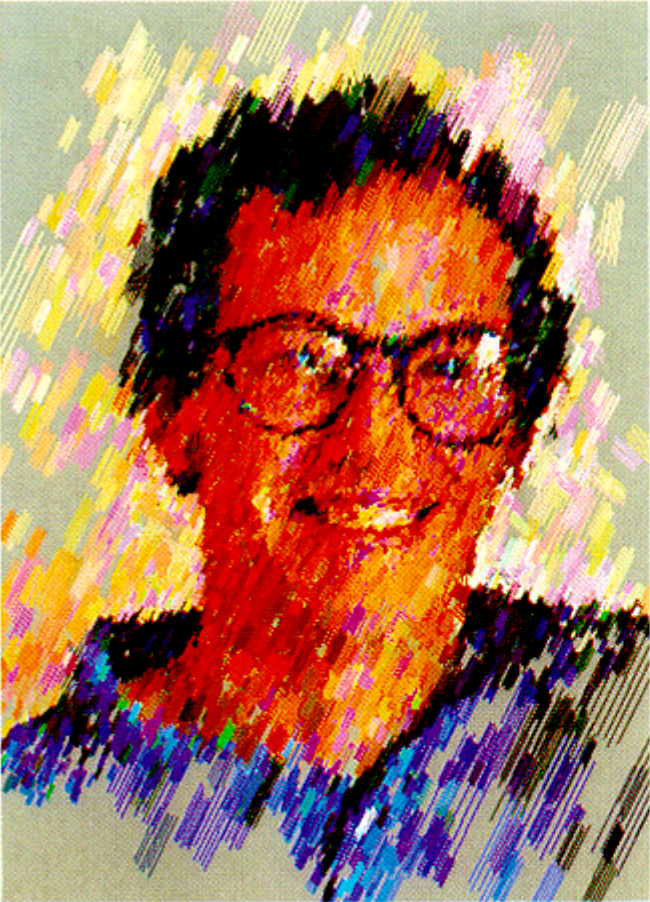
\includegraphics{haeberlihandcrafted}
    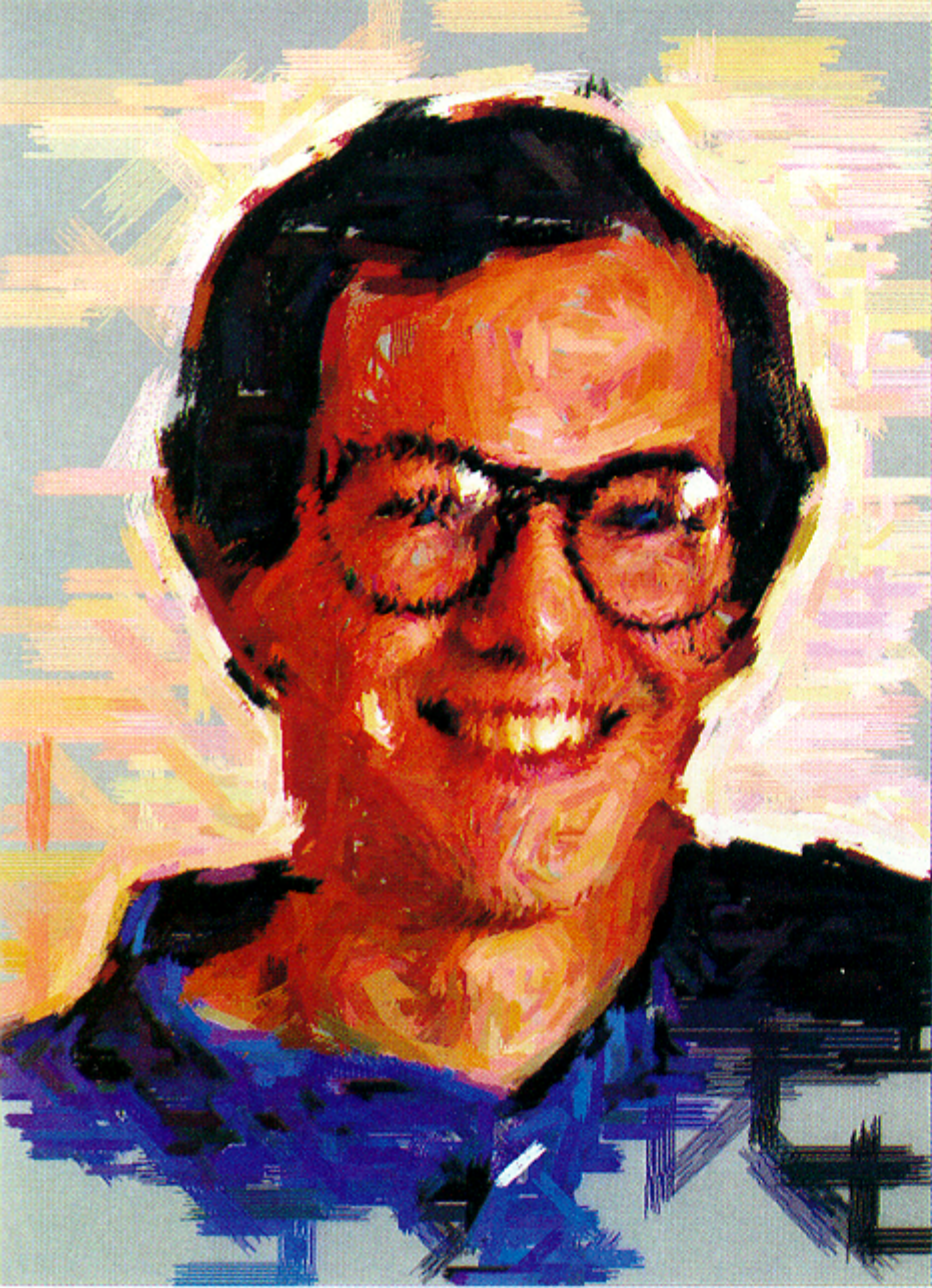
\includegraphics{haeberligradientdriven}
    \caption[]{Interactively painted images using \citeauthor*{paintbynumbers}'s method with a hand-selected orientation (\reffig{handselected}) and a gradient-driven orientation(\reffig{gradientdriven}).}
    \labfig{haeberliportrait}
\end{marginfigure}
\citeauthor*{paintbynumbers} even introduced the use of a scanned brush stroke texture in his algorithm.
\begin{marginfigure}
    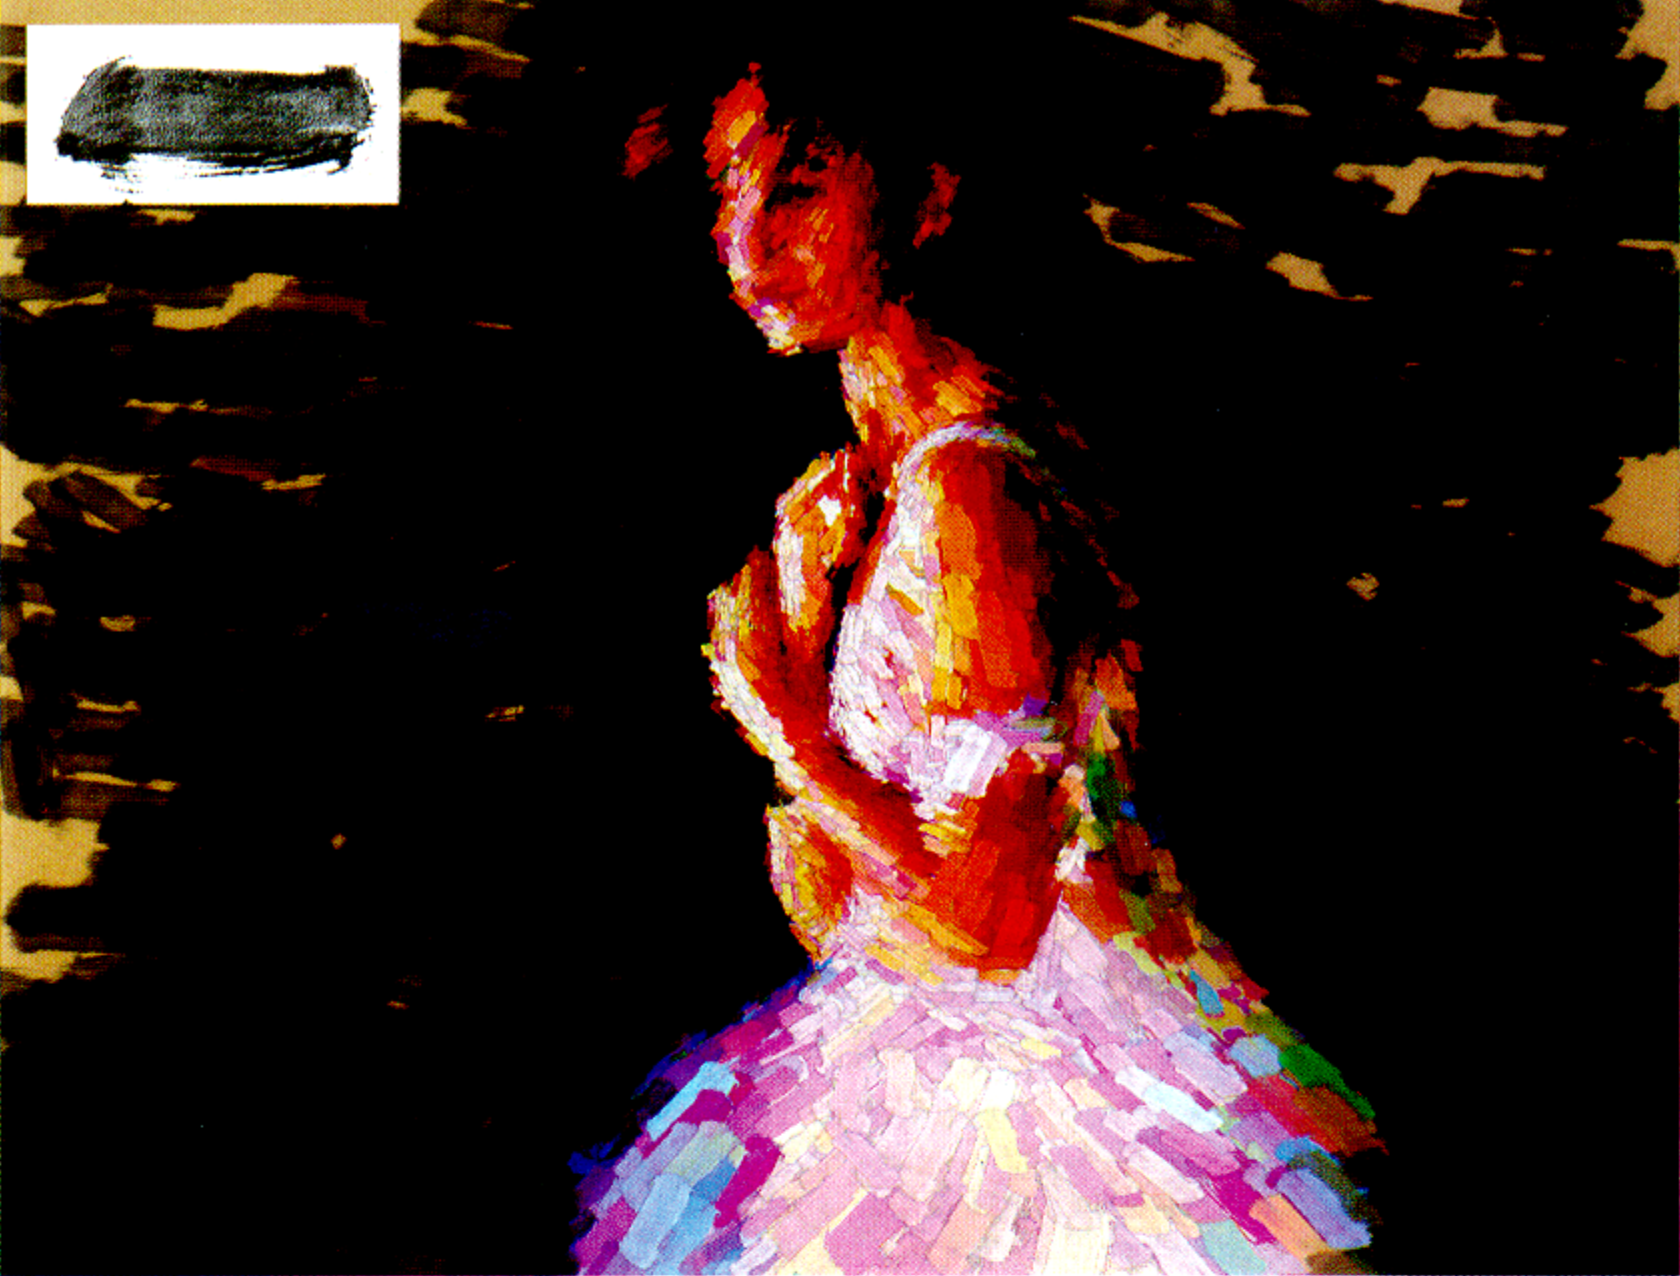
\includegraphics{haeberlibrushstroke}
    \caption[]{Rendered image with a brush stroke texture}
    \labfig{haeberlitexture}
\end{marginfigure}

Additionally to his interaction-based approach, \citeauthor*{paintbynumbers} also introduced a relaxation based approach \cite{paintbynumbers}.
In this approach a given set of 100 brush strokes is iteratively perturbed.
If the perturbation minimizes the energy function (L2-distance), the perturbation is kept.
If not, another perturbation is applied.
\begin{marginfigure}
    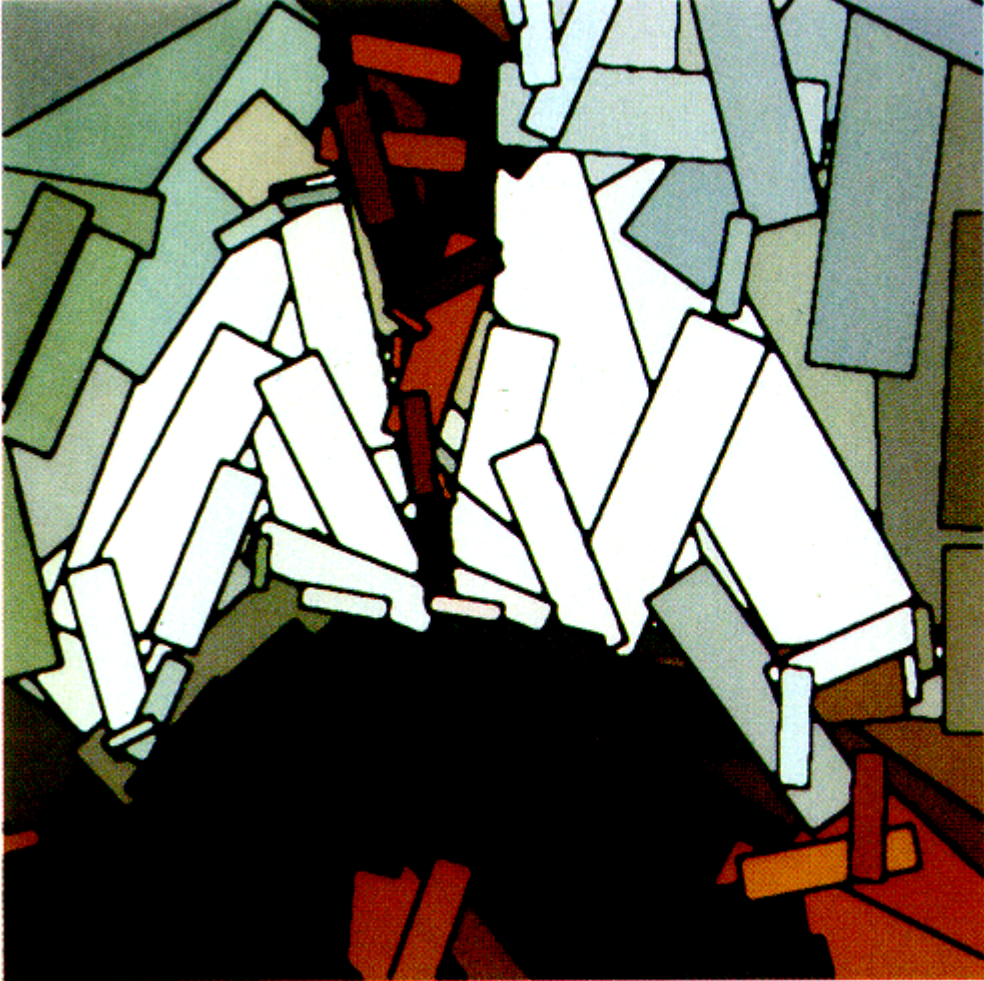
\includegraphics{haeberlirelaxation}
    \caption[]{Image approximated by relaxation.}
    \labfig{haeberlirelaxation}
\end{marginfigure}
This is described by \citeauthor*{hertzmannreview} as trial-and-error algorithm and very similar to genetic algorithms which shall be explained later \cite{hertzmannreview}.

Based on \citeauthor*{paintbynumbers}'s work, other authors automated the process of stroke positioning.
At the same they improved various aspect of brush strokes which were well categorized in a review by \citeauthor*{PRreview}.
The relevant categories are position, path and orientation, length and width, ordering, and color \cite{PRveview}.

%litwinowicz
\citeauthor*{apple} proposed a straight-forward way of placing brush strokes evenly spaced over the entire image.
Parameters are then inferred similar to \citeauthor*{paintbynumbers}'s approach.
To give a more random feel to these brush strokes, the obtained parameters are randomly perturbed according to preset parameters.
Also, a weakness of orienting brush strokes perpendicular to the gradient is dealt with.
For large uniform areas with little to no gradient, the orientation could become arbitrary.
\citeauthor*{apple} proposes to refine the gradient field by interpolating between the boundaries of large uniformly colored areas.
Also, \citeauthor*{apple} introduced temporal coherence to brush strokes, which meant that brush strokes move with the optical flow between frame in a video.

%hertzmann
\citeauthor*{hertzmann} reformulated the problem as an energy minimization problem in two publications \cite{hertzmanreview, Hertzmann}.
\begin{align}
    E(R) & = E_{\text{recon}}(R) + E_{\text{area}}(R) + E_{\text{nstr}}(R) + E_{\text{cov}}(R) \\
    E_{\text{recon}}(R) & = \sum_{x \in W, y \in H} w_{\text{recon}}{}_{x, y} \norm{I_{x, y}(R) - I_{x, y}}^2_2 \\
    %E_{\text{area}}(R) & = w_{\text{area}} \sum_{r \in R} \text{area){r} \\
    %E_{\text{nstr}}(R) & = w_{\text{nstr}} (\text{\#R}) \\
    %E_{\text{cov}}(R) & = w_{\text{cov}} (\text{\#empty pixels in $I(R)$}) \\
\end{align}
where $R$ is a brush stroke representation, $I$ is the target image, and $I(R)$ is the rendered representation.
$x$ and $y$ are pixel positions.
By adjusting the different weights, properties of the rendering can be altered.
$w_{\text{recon}}$ can vary spatially and dictate how well the reconstruction must fit the original image in certain areas.

Additionally, he added long strokes as B-splines with arbitrary control points.
In contrast, \citeauthor*{paintbynumbers} and \citeauthor*{apple} argued that short straight brush strokes would aid the perception of impressionistic style.
Furthermore, \citeauthor*{Hertzmann} added advanced rendering for brush strokes with synthetic textures in his work \cite{Hertzmann}.

\citeauthor*{Hertzmann} combined all these aspects in his approach with advanced relaxation methods similar to \citeauthor*{paintbynumbers}.
Based on trial-and-error search, \citeauthor*{Hertzmann} samples a local region along the many dimensions that represent a single brush stroke.
The best set of parameters that minimizes the energy function $E$ is then picked as new parameters.

In order to achieve better visual quality \citeauthor*{Hertzmann} also employs a coarse-to-fine multi-layer rendering approach.
Hereby, he blurred the image in the early iterations of his method and fixed the brush size at a large value.
Blurring of the image would then be gradually reduced along with the brush size.
The final implementation is further optimized to accelerate the relaxation algorithm and allow for more brush strokes than \citeauthor*{paintbynumbers}'s approach.

Ultimately, \citeauthor*{Hertzmann} achieves respectable results with his approach and many ideas of this thesis can be found in his works as well.

\subsubsection{Stroke Rendering}

%FOCUS ON QUALITY OF STROKES
%physical simulations
%Lee et al, baxter et al focused on 3D version of bristle

%there are papers which focus on the material i.e. paper etc.

%later



\subsection{Filter-Based Rendering}
%IMAGE PROCESSING BASED TECHNIQUES
Parallel to his works in stroke-based rendering, \citeauthor*{imageanalogies} proposed a way of stylizing images much faster by using trainable filters.
They call their technique 'image analogies' since the transformation between two training images is analogously applied to a test image.

Basically, for creating the impression of brush strokes a photograph $A$ and a painting of that photograph $A'$ is needed.
As this is rarely the case, \citeauthor*{iamgeanalogies} showed that using anisotropic diffusion works also reasonably well to generate $A$ from $A'$.
Then their algorithm searches locally for the best filter parameters $F(p)$ that transform $A(p)$ into $A'(p)$.
$p$ is an arbitrary position in the image.
By using another search algorithm to match similar regions $B(p)$ and $A(p)$, $F(p)$ can be used to transform $B(p)$ into $B'(p)$.
Thus $B'$ a stylized version of $B$ can be obtained by transforming it analogously to $A \rightarrow A'$.
%Hertzmann et al 2010 smooth a painting and optimize filter parameters for the inverse transformation -> apply the filters to photos
    %similar to superresolution and texture synthesis
%first approach is just grouping pixels simialrly to super-pixels
Other works like \citeauthor*{texturetransfer}~\cite{texturetransfer} have built on this principle idea which has led to a fast texture transfer algorithm \cite{fasttexturetransfer}.
Besides only matching local region according to their pixel values, \citeauthor*{texturetransfer} obtain a flow map (which they call 'directions'), that is based on the content image's gradient.
This flow is then also matched against the style image.
\begin{figure}
    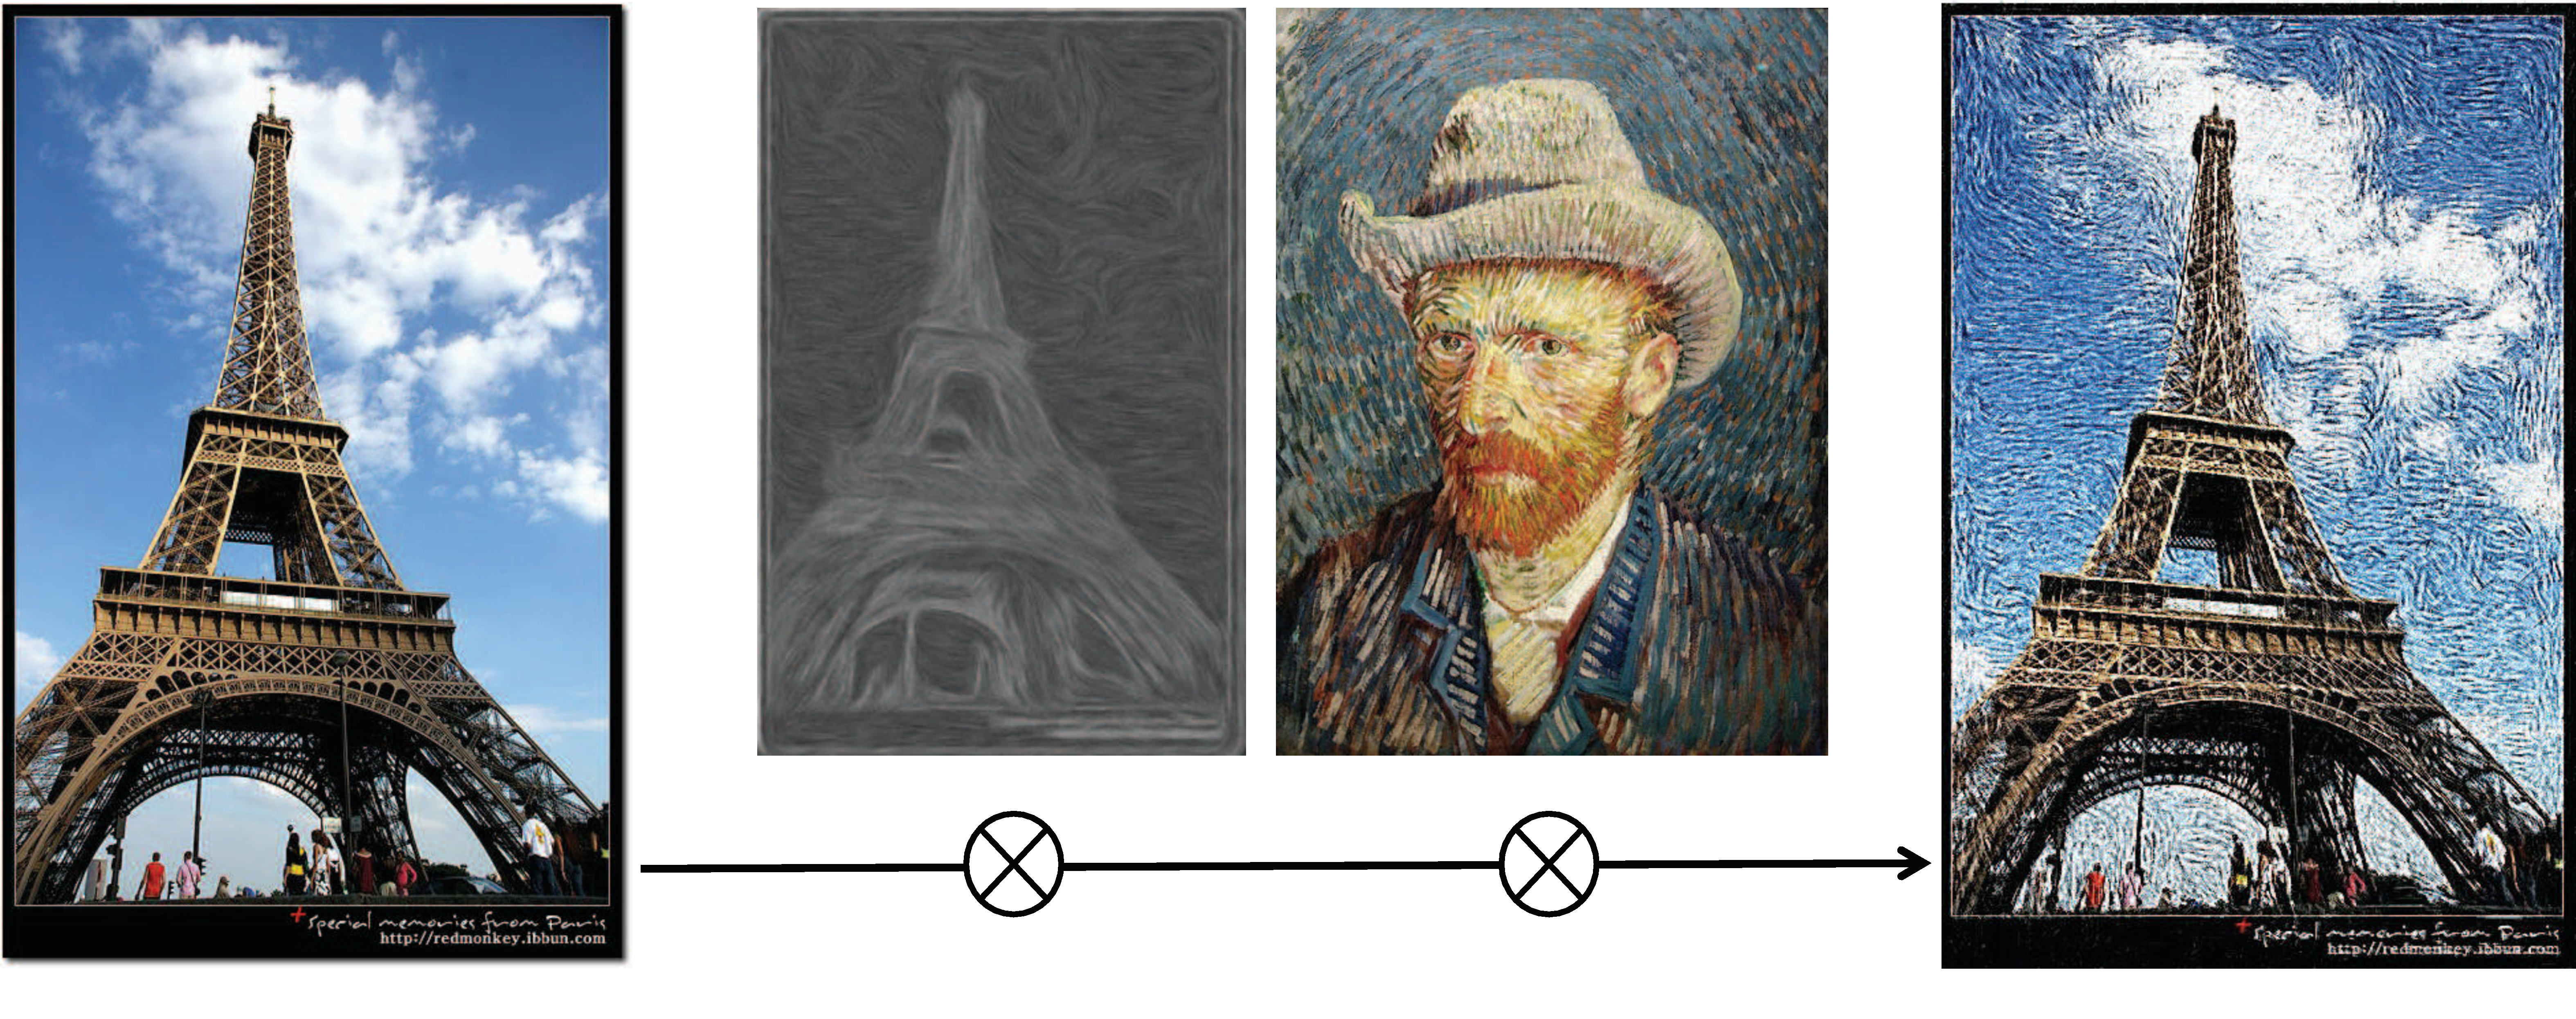
\includegraphics{texturetransfer}
    \caption[]{Target image $T$ is combined with a dictional map specially obtained from $T$ and a style image  $S$. The result maintains the direction's flow while presenting the texture from $S$.}
    \labfig{texturetransfer}
\end{figure}

%Lee et al 2010 transfer the texture of brush stroke onto an image much like style transfer (this is the intersection)


\subsection{Drawing Networks}
%gaining traction

%were described by hertzmann as greedy algorithms.

%learning2Paint
%SPIRAL
%DrawNet
%PaintNet


%image transofrmation tasks denoising, colorization, super-resolution, semantic-segmentation, depth estimation, 

\subsection{Genetic Algorithms}
Genetic algorithms are typically not closely associated with painterly rendering, even though they represent just a different approach to algorithms for this problem.

Genetic algorithms already perform a similar task in order to approximate images by other geometric shapes or even smaller photos (also known as the popular photo mosaic effect).
Starting with a random set of circles that are parameterized by their position, radius, and color, it then chooses the most successful samples and resamples in a region around these.
This process is repeated until a certain level of convergence is reached.

%refer to neural style transfer: a review

\begin{marginfigure}
    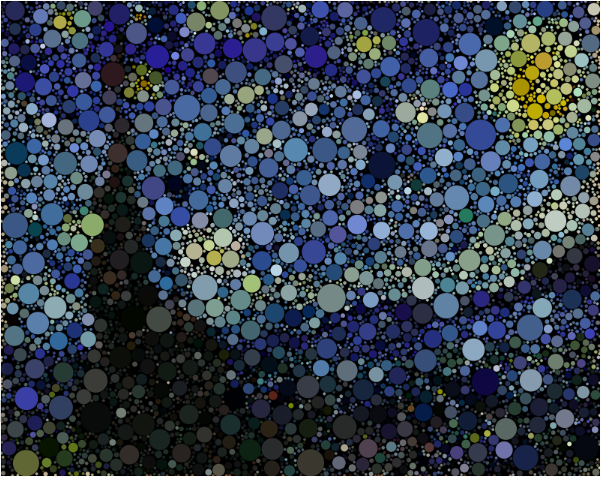
\includegraphics{genetic_starry_night}
    \caption[]{Starry Night approximated by a genetic algorithm using only circles. \url{https://effyfan.com/2018/03/02/w6-van-gogh-flowfield/}}
    \labfig{genetic}
\end{marginfigure}

As well as this does work, it is very much computationally expensive as most samples will not fit the image, thus searching for the small set of fitting shapes requires to evaluate all the wrong shapes as well.
Considering artworks, brushstrokes have many more degrees of freedom, and artworks usually consist of upwards of a few thousand brushstrokes.
Consequently, it would be considerably more challenging to apply to this problem until computational resources have become a few magnitudes more powerful.

\begin{figure}
    \includegraphics{photomosaic_starry_night}
    \caption[]{Photo mosaic of Starry Night using only images by the Hubble Space Telescope. \url{http://www.astro.uvic.ca/~alexhp/new/figures/starrynight_HST.001.jpg}}
    \labfig{photomosaic}
\end{figure}

\section{Style Transfer}
\labsec{ST}

This field of style transfer has its origins 
%most active field
%style and texture are similar problem

\subsection{Early Approaches}
Earliest approaches
%painterly rendering is some kind of style transfer but shall be dealt with explicitly
%focus is on approaches that work only with pixels
%filters
%texton based approaches

%Some early approaches include histogram matching on linear filter responses [19] and non-parametric sampling [12, 15].
%       . Pyramid-based texture analysis/synthesis
%       Split and match: example-based adaptive patch sampling for unsupervised style transfer
%       Image quilting for texture synthesis and transfe
%low-level statistics and fail to perceive semantic structures



\subsection{Neural Style Transfer}
%A bit similar to transfer learning -> utilize the pretrained features especially of the early layers.
The field of style transfer has really gained traction in 2015 with the publication of \textbf{A Neural Algorithm for Artistic Style} by \citeauthor*{gatys}.
It was the first approach to transfer the style of one image to another and at the same time maintaining a high contextual fidelity.
In retrospective, this work really kicked off neural style transfer as a field.

\citeauthor*{gatys} themselves pinpoint the novelty of their approach as 'manipulations in feature spaces' as opposed to previous approaches that 'directly manipulate the pixel representation of an image'\cite{gatys}.
They use existing neural architectures and extract information in two separate ways, such that content and style can be separated.

Previous works already used \textbf{perceptual loss} to accumulate information on the content in an image \cite{percep_loss}, or check whether two images have the same content \cite{other_percep_loss}.
%networks trained on object recognition increasingly care about the content with every layer
Perceptual loss is based on the VGG-19 architecture \cite{VGG} which is a deep CCN trained for object classification on ImageNet \cite{imagenet}.
By arguing that the network's layer activations increasingly respond to the content when following the networks' hierarchy.
Some much even, that it is possible to reconstruct the content of an image by using the activations of one such layer.

For reconstruction of an image's content, gradient descent is performed on a white noise image.
The gradient descent aims to minimize the perceptual distance between the reconstruction and the target image.
Perceptual distance is defined as the L2-distance between the activations of two images in deep layer of the VGG-network.

For image vector $\vec{x}$ with $\vec{x} \in = \R^{M_0}, M_0 = H_x \dot W_x $, a layer $l$ of the network has $N_l$ feature maps of size $M_l$.
In this case $M_l$ is equal to the height times the width of the feature map of the $l$-th layer.
The activations of the $i$-th filter ($i \in N_l$) at position $j$ ($j \in M_l$) at layer $l$ can then be represented by matrix $F(\vec{x})_{ij}^l \in \R^{N_l \times M_l}$.
The perceptual distance is then defined as
\begin{align}
    d_{\text{percep}}(\vec{x}, \vec{y}) = \sum_{i, j} (F(\vec{x})_{ij}^l - F(\vec{y})_{ij}^l)^2 = \norm{\tensor{F(\vec{x})}^l - \tensor{F(\vec{y})}^l}_2^2
\end{align}
, which allows to define the perceptual loss or content loss as 
\begin{align}
    \L_{\text{content}} = \frac{1}{2} \sum_{i, j} (F(\vec{x})_{ij}^l - F(\vec{y})_{ij}^l)^2 = \frac{1}{2} \norm{\tensor{F(\vec{x})}^l - \tensor{F(\vec{y})}^l}_2^2
\end{align}

\marginnote{The factor $\frac{1}{2}$ will cancel out when deriving $\L_{\text{content}}$ with respect to $F(\vec{x})_{ij}^l$.}

Minimizing the content loss between two images, by using gradient descent the content of an image can be restored (see \reffig{content_style_loss}).

\begin{figure*}
    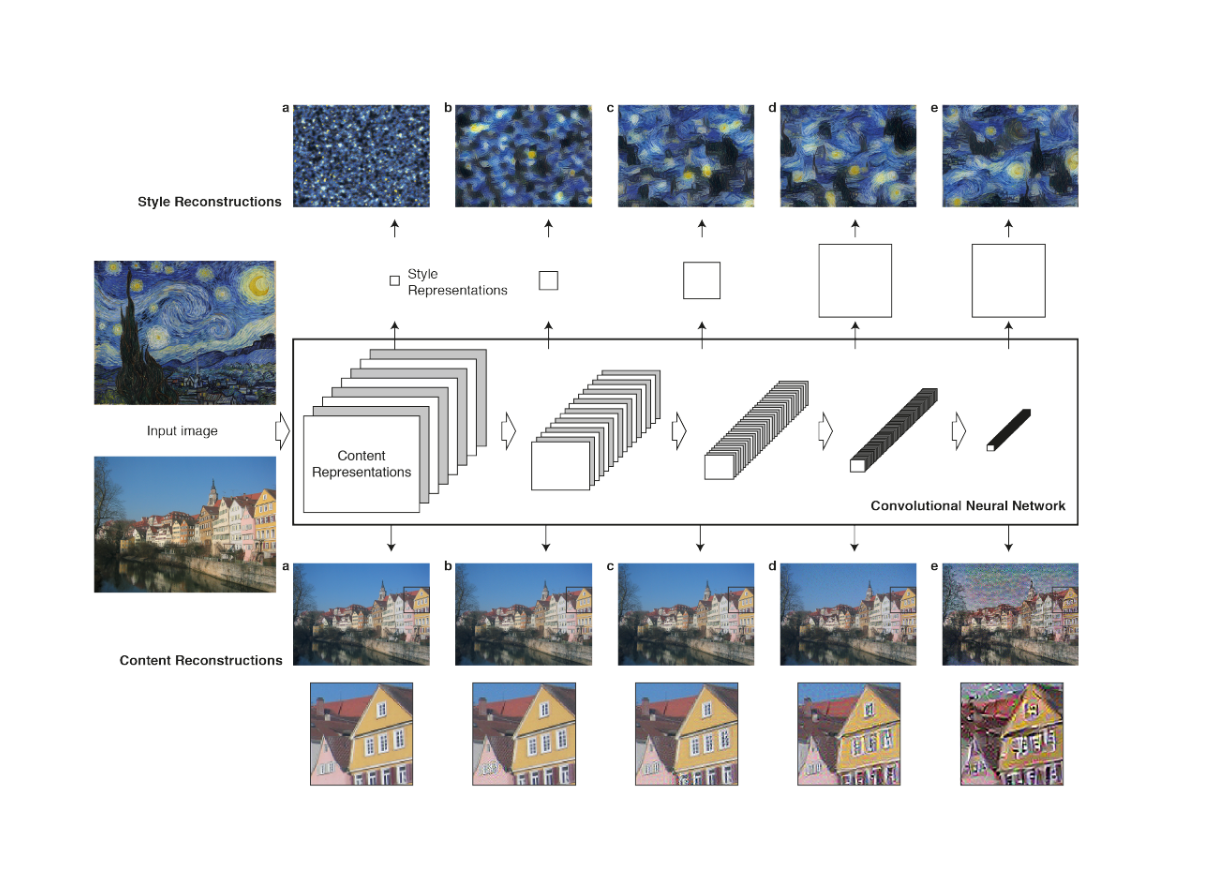
\includegraphics{content_style_loss}
    \caption[]{Reconstructions of content(bottom) and style(top) using different layers. \cite{gatys}}
    \labfig{content_style_loss}
\end{figure*}

As approximating the content of an image has now become possible, the question is whether this is possible with style as well.
\citeauthor*{gatys} again turned to the pre-trained VGG network for this.
They explicitly reduce style to texture for this reason and thus search for a feature space that captures \textbf{texture} rather than content.
Subsequently, \citeauthor*{gatys} propose the use of \textbf{Gram matrices} as they capture the correlations of feature-activations over their spatial extent.

The Gram matrix of a given matrix $\tensor{A}$ is the inner product of all column vectors in $\tensor{A}$.
\begin{align}
    G = \langle a_{i}, a_{j} \rangle = \tensor{A}^T \tensor{A} \text{ if $a_1$...$a_j$ are column vectors of $\tensor{A}$}
\end{align}
The resulting Gram matrix G now has the form $j \times j$ and captures texture information but no longer the global content.

\refsec{problem} already mentioned that style is very complex and exists at various scales at the same time which \citeauthor*{gatys} address by using many layers.
As these layers sit at different depths their field of view varies and each layer captures information at a different scale.
Early layers will tend to hold small scale information, later layers will hold larger scale information with every layer.

\citeauthor*{gatys} first compute the Gram matrices each layer $l$ for both the target style image and the current image.
Then they use the L2 distance metric to measure the discrepancy between them.
\begin{align}
    G(\vec{x})^l & = \frac{1}{(2 N_x^l M_x^l)^2} F(\vec{x})^l{}^T F(\vec{x})^l \\
    G(\vec{y})^l & = \frac{1}{(2 N_y^l M_y^l)^2} F(\vec{y})^l{}^T F(\vec{y})^l \\
    d_{\text{style}}^l(\vec{x}, \vec{y}) & = \norm{G(\vec{x})^l - G(\vec{y})^l}^2_2 \\
\end{align}

\marginnote{The denominator of $\frac{1}{4 N_x^l{}^2 M_x^l{}^2}$ is squared since the Gram matrix is the product of a matrix with itself transposed.}

The style distances at each layer are then weighted and summed up to make up the style loss:

\begin{align}
    \L_{\text{style}} = \sum_{l} w_l d_{\text{style}}^l(\vec{x}, \vec{y})
\end{align}

%again one can visualize the style/texture that is perceived
This style loss can again by used together with gradient descent in order to check whether it is possible to reconstruct the texture of an image much like the content of an image.
\reffig{content_style_loss} shows that it is in fact possible to reconstruct the texture of the image at various scales.
Specifically the local consistency of each texture becomes larger, the deeper the layer sits.

%mix content and style
\citeauthor*{gatys} now combine the losses for one content image $\vec{c}$ with a style image $\vec{s}$ and optimize $\vec{x}$ in the same way the reconstructions have been obtained.

\begin{align}
    \L_{\text{total}} = \lambda_{\text{content}} \L_{\text{content}}(\vec{x}, \vec{c}) + \lambda_{\text{style}} \L_{\text{style}}(\vec{x}, \vec{s})
\end{align}

\begin{marginfigure}
    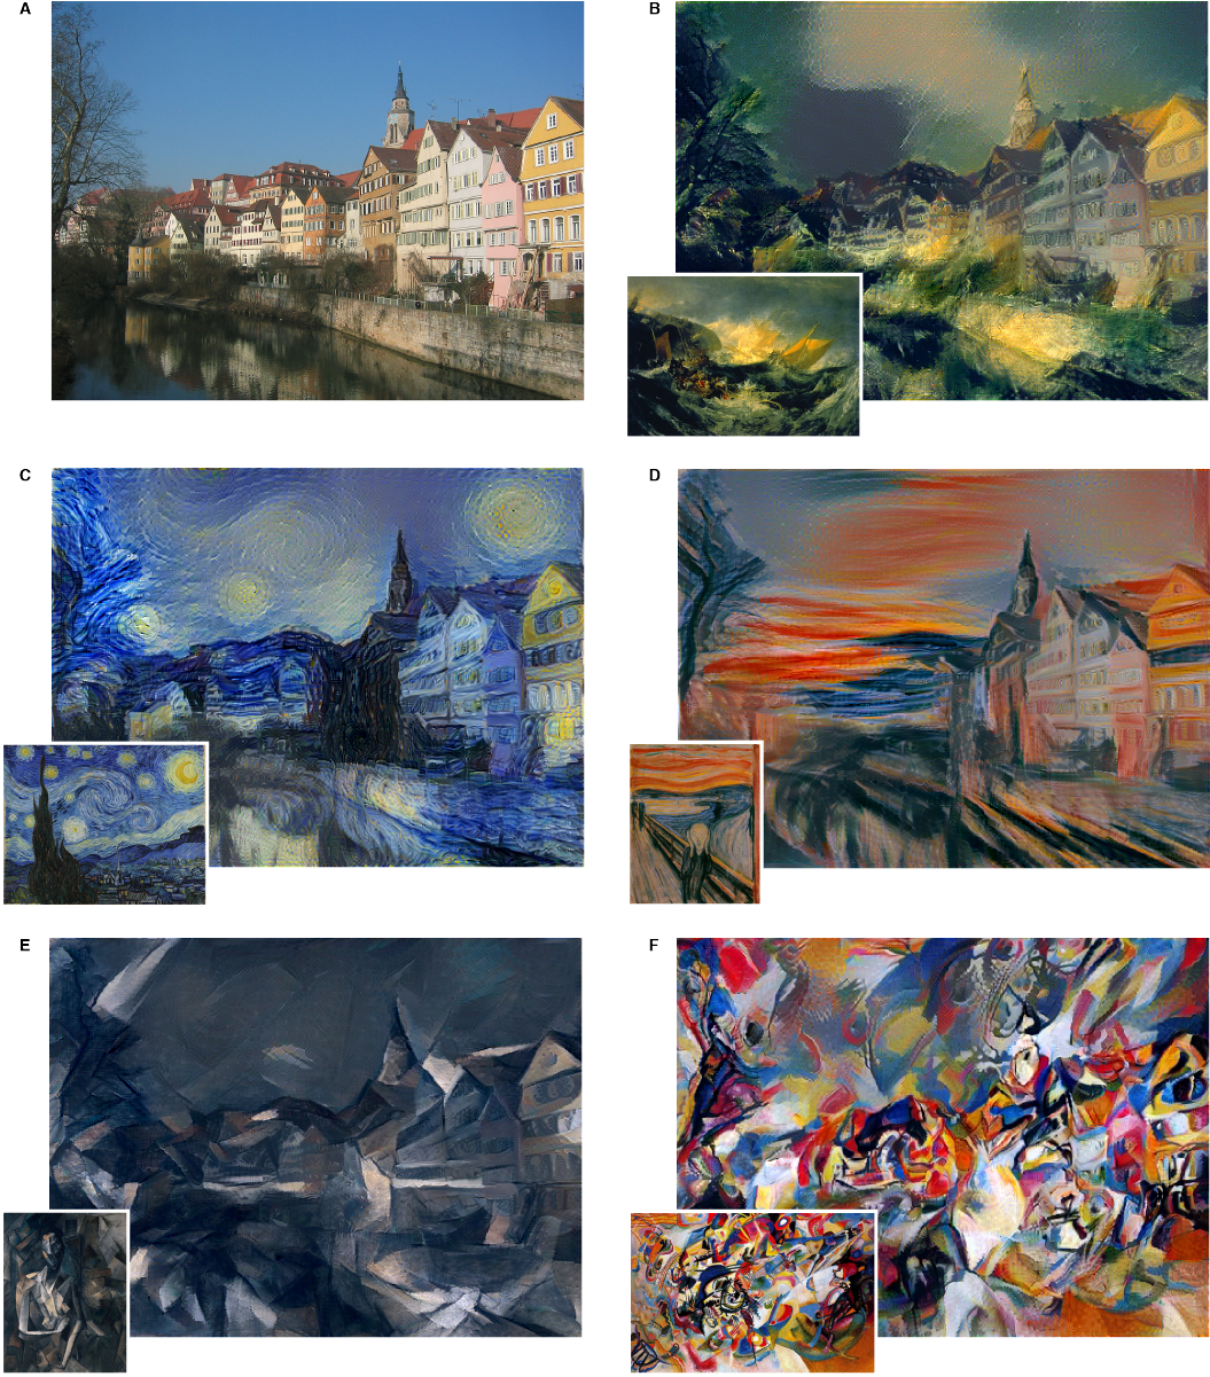
\includegraphics{gatys_ST}
    \caption[]{Style transfer examples by \citeauthor*{gatys}. \cite{gatys}}
    \labfig{content_style_loss}
\end{marginfigure}

The result of this can be seen in \reffig{gatys_ST}

\subsubsection{Follow-Up Research}
There has been some follow-up research on \citeauthor*{gatys}'s work which addresses mainly how the style loss works.

\citeauthor*{MMD} have shown that the style loss is equivalent to calculating the \textbf{maximum mean discrepancy (MMD)} between the features of each layer \cite{MMD}.
MMD is a test-statistic for a null hypothesis $p=q$ with the data $X = \{x_i\}^n_{i=1}$, sampled from $p$, and $Y = \{y_i\}^n_{i=1}$, sampled from q, at hand.
It can be used as a difference measure as well and vanishes only if $p=q$.
\begin{align}
    \text{MMD}^2[X, Y] & = \frac{1}{n^2} \sum^n_{i=1} \sum^n_{i'=1} k(\vec{x}_i, \vec{x}_{i'}) \\
    & + \frac{1}{m^2} \sum^m_{j=1} \sum^m_{j'=1} k(\vec{y}_j, \vec{y}_{j'}) \\
    & - \frac{2}{nm} \sum^n_{i=1} \sum^m_{j=1} k(\vec{x}_i, \vec{y}_{j})
\end{align}

MMD can be based on different kernel functions $k$ and \citeauthor*{MMD} have shown that the style loss is equivalent to the squared MMD with a polynomial kernel.
Consequently they were able to show, that style transfer work with different kernel functions as well and even by explicitly matching the batch statistics (see \reffig{MMD}):
\begin{align}
    d_{\text{style}}^l(\vec{x}, \vec{y}) & = \frac{1}{N_l} \sum_{i = 1}^{N_l} \left( (\mu^i_{F(\vec{x})^l} - \mu^i_{F(\vec{y})^l}) + (\sigma^i_{F(\vec{x})^l} - \sigma^i_{F(\vec{y})^l}) \right)
\end{align}

\begin{figure}
    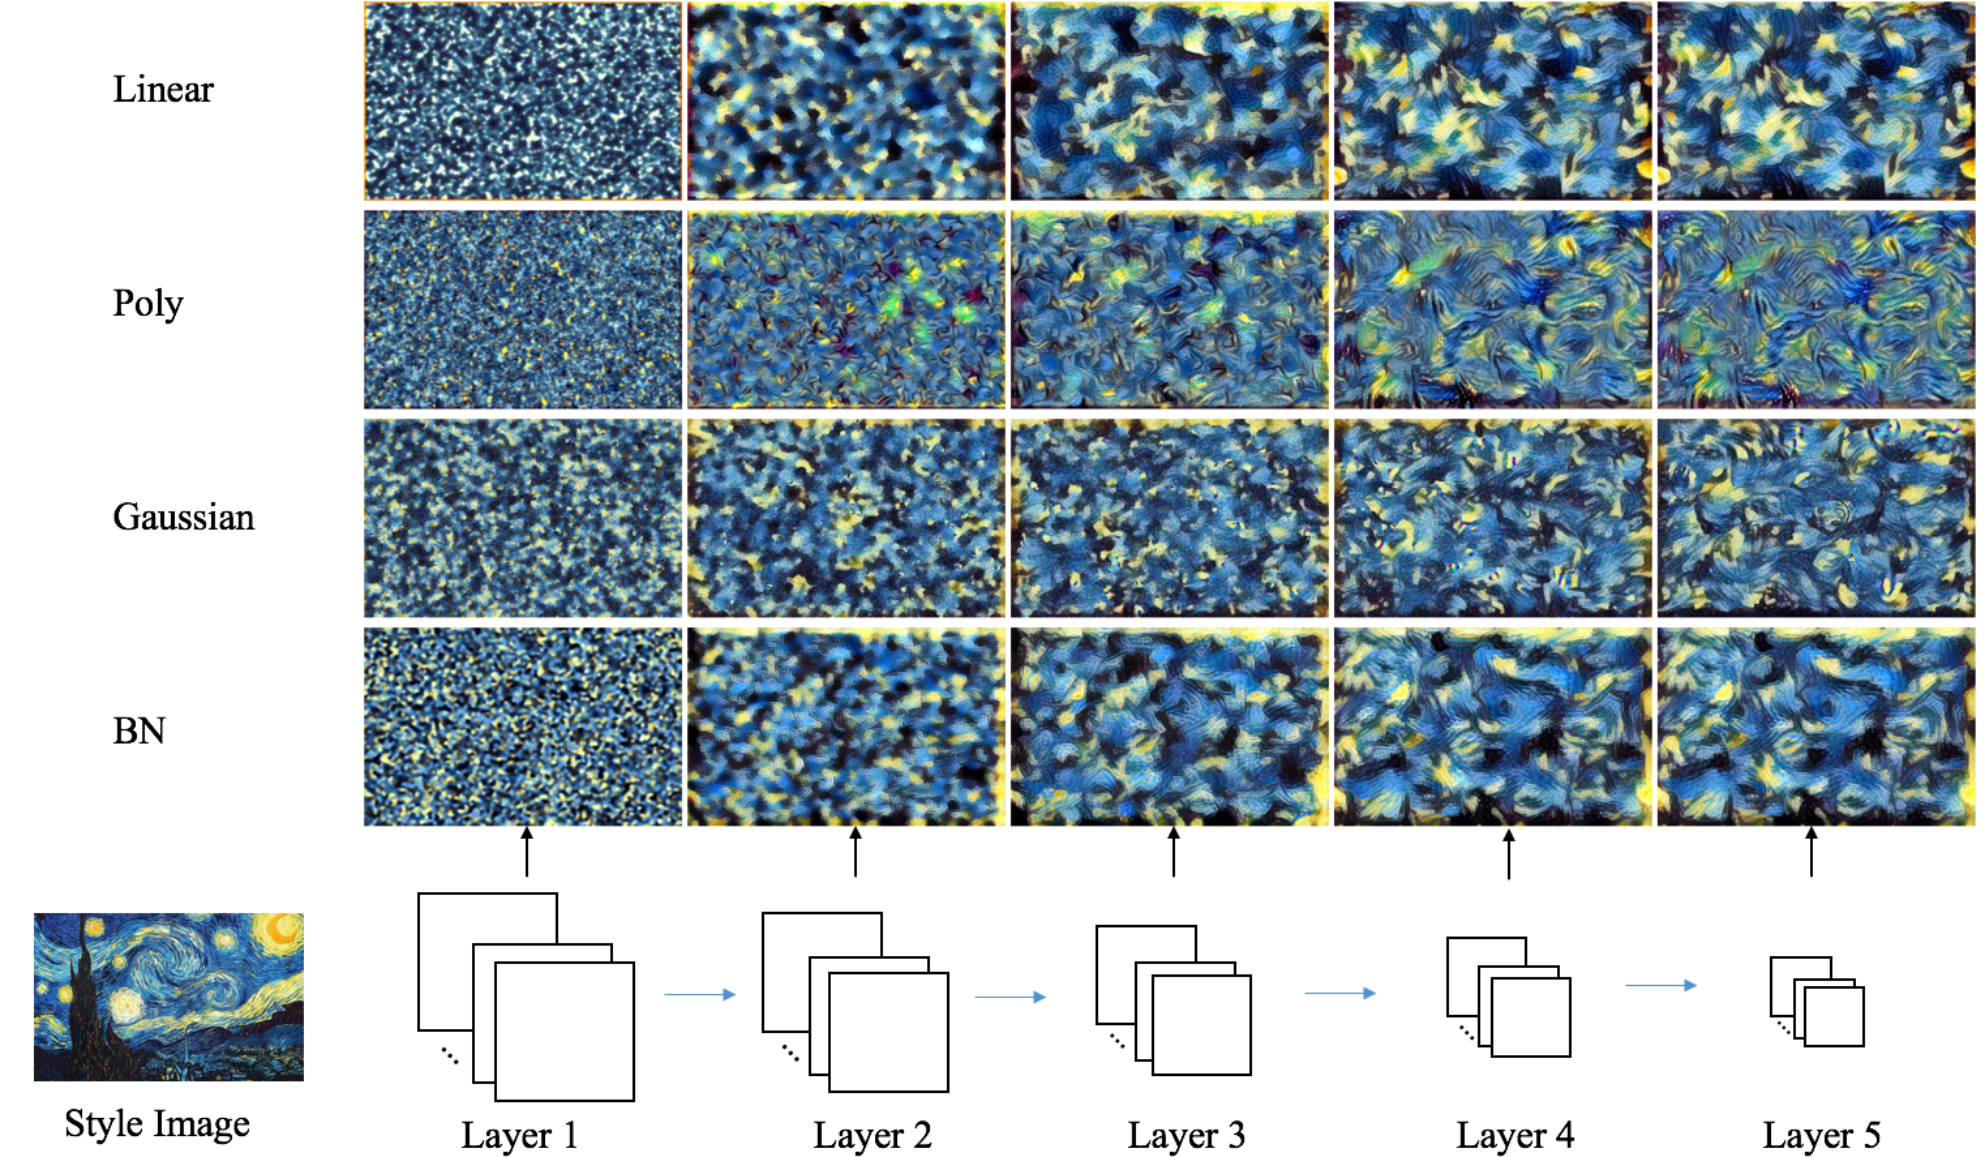
\includegraphics{MMD}
    \caption[]{Reconstructed textures for Starry Night using different kernel functions $k$ \cite{MMD}}
    \labfig{MMD}
\end{figure}


\citeauthor*{LenDu} tested whether pre-trained weights play an important role when performing style transfer.
He was able to show basic style transfer even with random initialized networks, but results vary wisely depending on the random initialization.
Ultimately, it is possible so obtain some style transfer with this technique but the pre-trained weights seem to play an important role in stablizing the reconstruction process.

\subsection{State of the Art}

\subsubsection{Real-Time Style Transfer}
%johnson
Following \citeauthor*{gatys} seminal work, other have followed suit in trying to stylize images with neural networks.
\citeauthor*{Johnson} were the first to use the same losses but train a feed-forward architecture with it \cite{johnson}.
They were able to significantly speed up the stylization process like this as stylization was performed in a single feed-forward pass instead of a lengthy gradient descent optimization.
Ultimately, this enabled them to generate stylized images in real-time from a given content image, using a deep residual convolutional neural network.
\begin{figure*}
    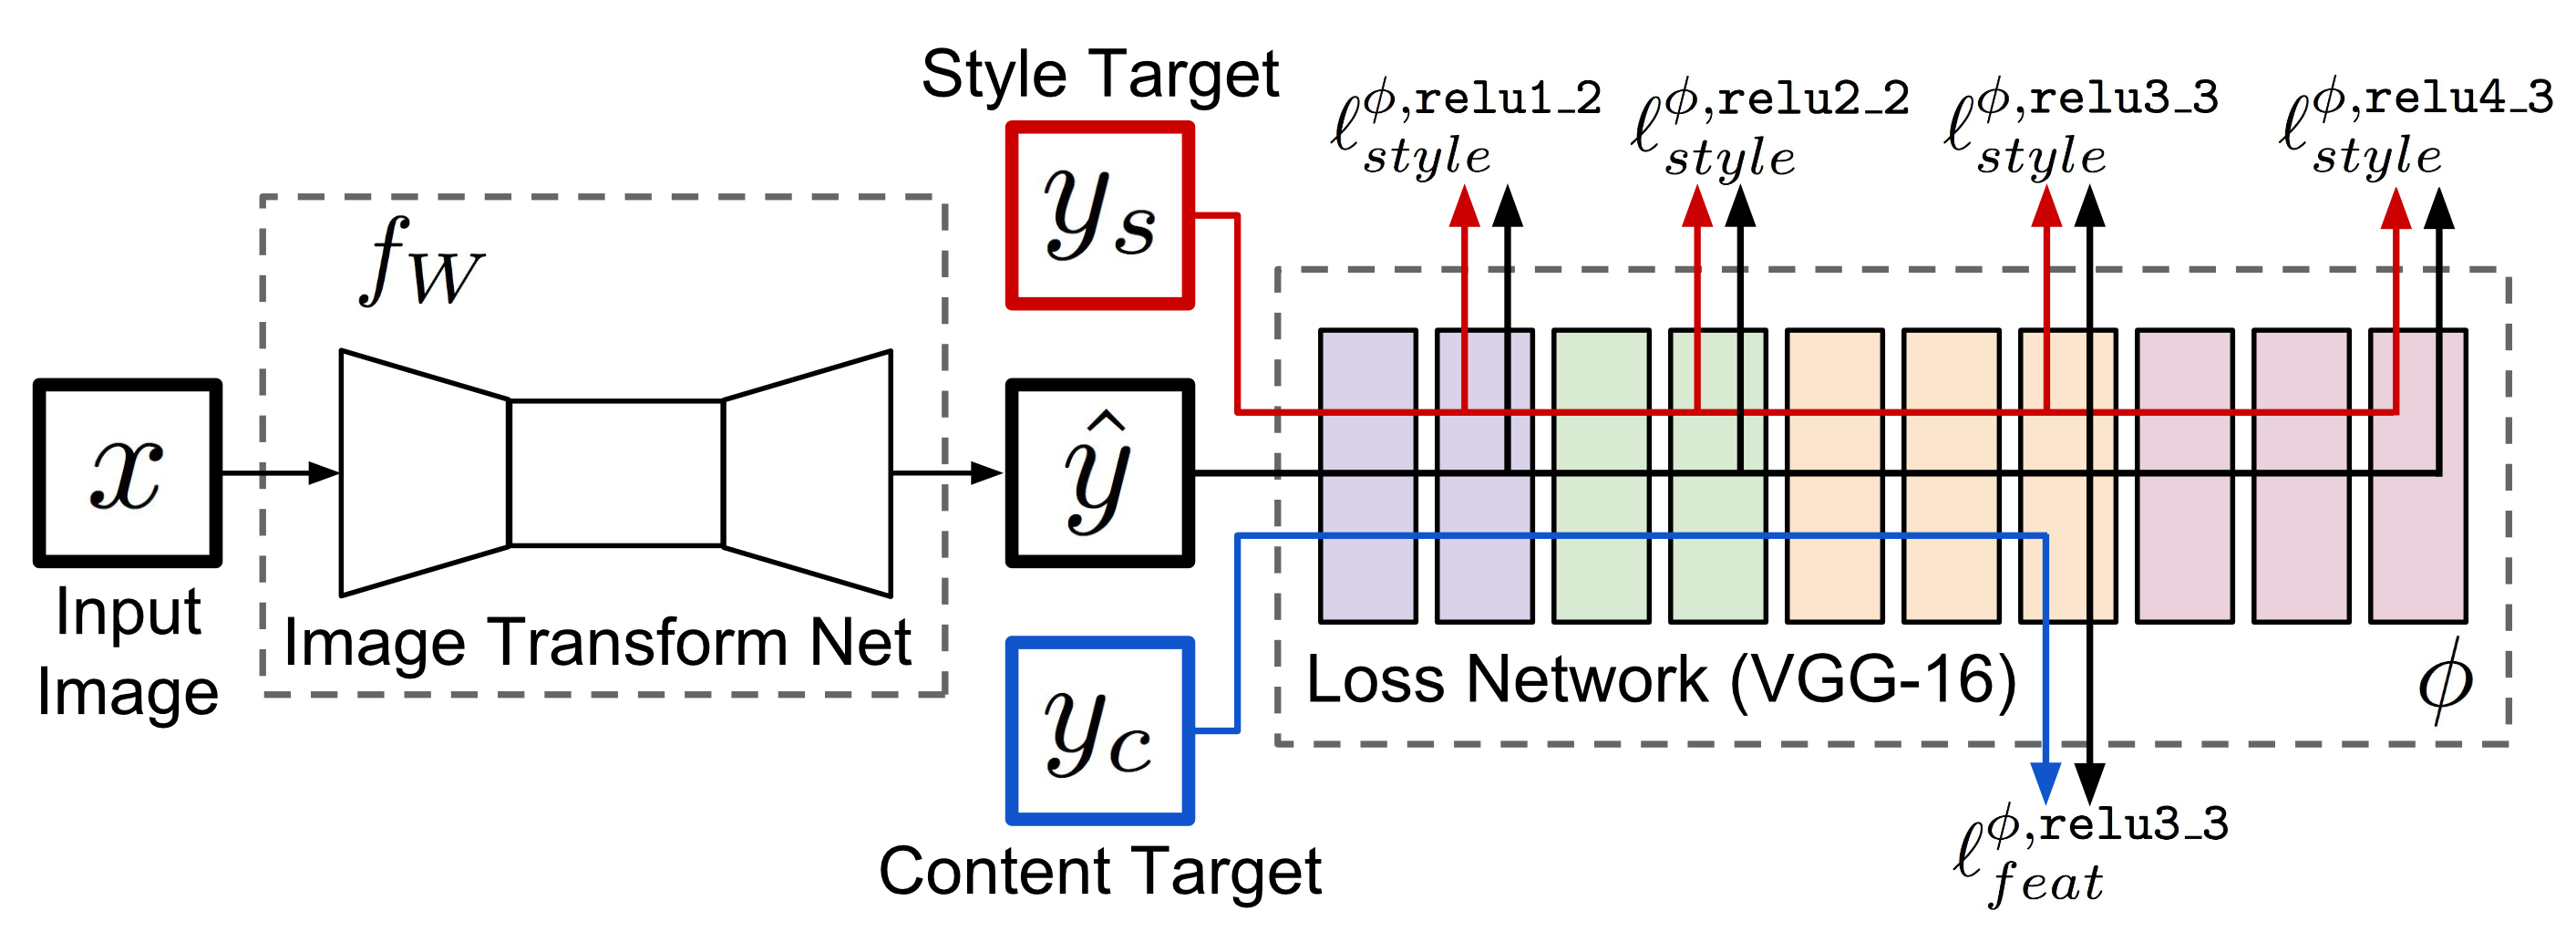
\includegraphics{johnson_net}
    \caption[]{Training set-up by \citeauthor*{johnson}. \cite{johnson}}
    \labfig{johnson_net}
\end{figure*}

%markov random field ansatz?

%adain
\subsubsection{Arbitrary \& Universal Style Transfer}
\citeauthor*{AdaIN} used a different feed-forward approach for arbitrary style.
They first encode an arbitrary style image $\vec{s}$ as well as a content image $\vec{c}$ using a pre-trained VGG network.
This allows them to obtain the activations at a very deep layer of the network $F^l(\vec{s})$ and $F^l(\vec{c})$.
Then they compute the second order statistics for both $\mu_F^l(\vec{s}), \sigma_F^l(\vec{s})$ and $\mu_F^l(\vec{c}), \sigma_F^l(\vec{c})$.
Using adaptive instance normalization (AdaIN), they rescale the content activations such that they match the statistics of the style activations.
\begin{align}
    F'^l = \sigma_F^l(\vec{s}) \frac{F^l(\vec{c} - \mu_F^l(\vec{c})}{\sigma_F^l(\vec{c})} + \mu_F^l(\vec{s}) 
\end{align}
Finally, they train a decoder that minimizes the style and content loss, as they have been proposed by \citeauthor*{gatys}.
They achieve comparable results to other style transfer approaches at a similar speed to \citeauthor*{johnson} while allowing for any target style eventhough only training only once.
\begin{figure*}
    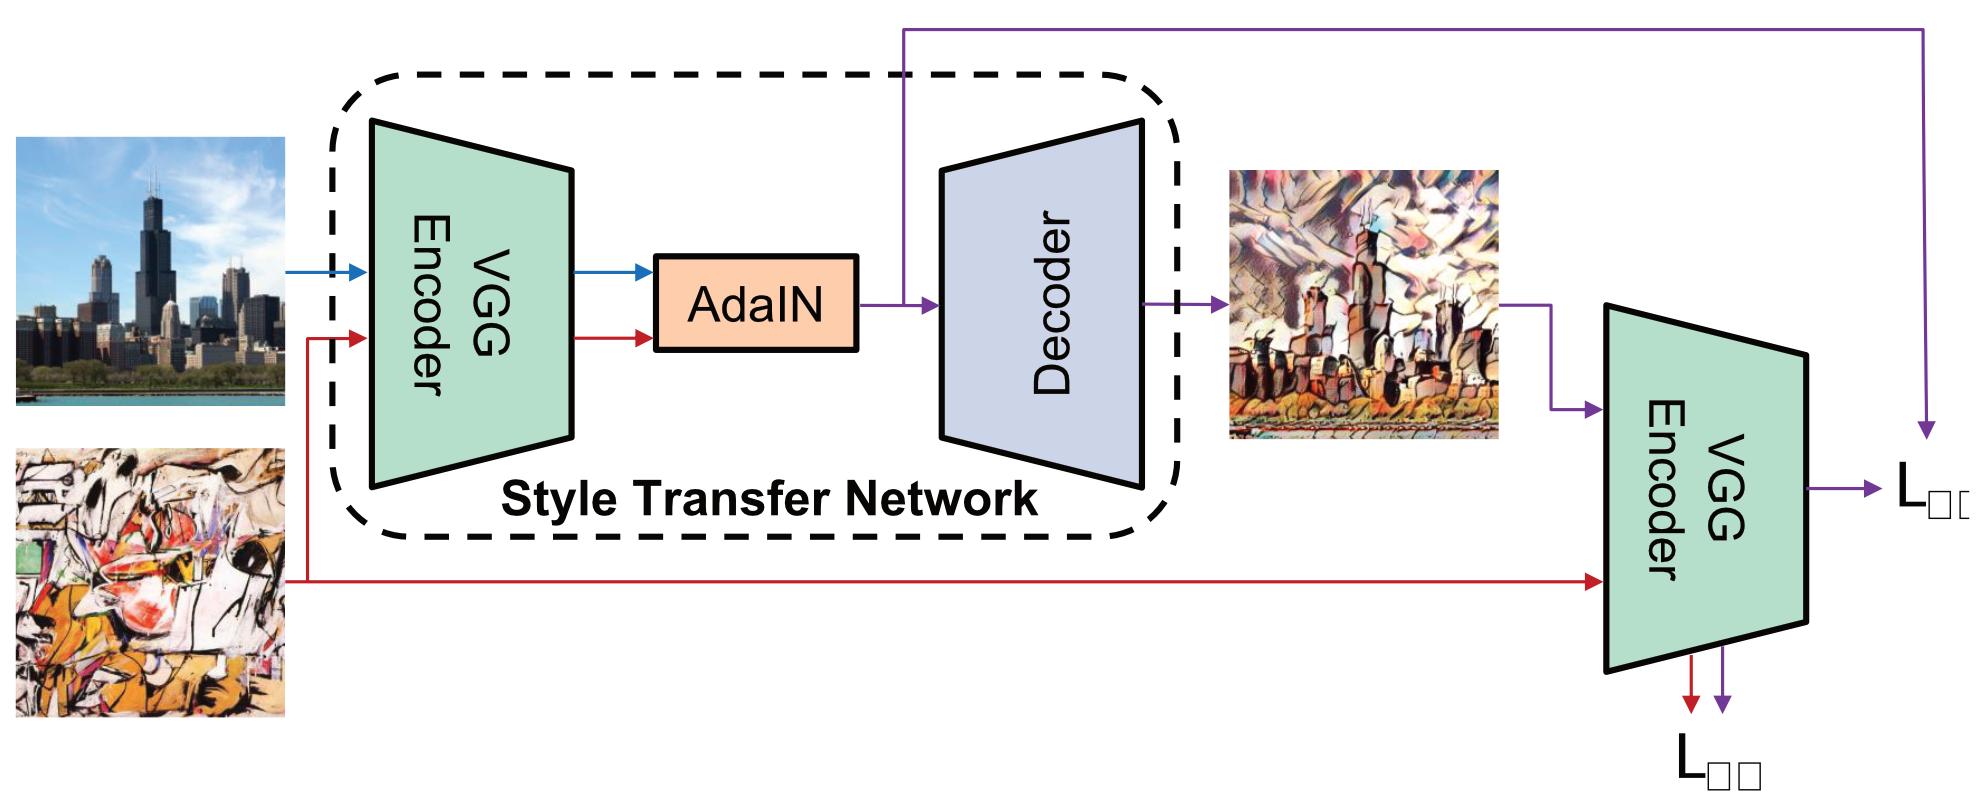
\includegraphics{adain_net}
    \caption[]{Training set-up by \citeauthor*{AdaIN}. \cite{AdaIN}}
    \labfig{johnson_net}
\end{figure*}

%wct
\todo{this is actually just PCA decompsition to a certain degree}
A similar approach by \citeauthor*{WCT} relies on matching the covariance and the mean of content and style activations.
They do that through what they call 'whitening and coloring transform' \cite{WCT}.
First they whiten $F^l(\vec{c})$ into $\hat{F}^l$ such that $\hat{F}^l \hat{F}^l{}^T = I$
\begin{align}
    \hat{F}^l = E_c D_c^{-\frac{1}{2}} E_c^T (F^l(\vec{c}) - \mu_c)
\end{align}
Where $D_c$ is the diagonal matrix of eigenvalues of the covariance matrix and $E_c$ is the respective orthogonal matrix of eigenvectors.
such that
\begin{align}
    F^l(\vec{c}) F^l(\vec{c})^T = E_c D_c E_c^T
\end{align}

Then coloring is performed by rescaling the whitened representation $\hat{F}^l$ into $\tilde{F}^l$
\begin{align}
    \tilde{F}^l = E_s D_s^{\frac{1}{2}} E_s^T \hat{F}^l + \mu_s \\
    F^l(\vec{s}) F^l(\vec{s})^T = E_s D_s E_s^T
\end{align}

The resulting $\tilde{F}^l$ is then decoded with a pre-trained decoder to render the final stylized result.
\citeauthor*{WCT} use pre-train the decoder solely on natural images and perceptual loss and reconstruction loss as objective.
Additionally, they introduce a pipeline that performs style transfer on multiple scales sequentially.
They achieve good results in real-time with just training the decoder once.

\subsubsection{Bidirectional Style Transfer}
%cyclegan
\citeauthor*{CycleGAN} went a different way on style transfer and rely on a generative adversarial objective to identify style in an image.
Specifically, they transform images between any two domains $x \in \mathcal{X}$ and $y \in mathcal{Y}$, not just photos and artworks.
For this, they use two discriminators ($D_X$ and $D_Y$, one for each domain) as well as two transformation networks ($G: X \rightarrow Y$ and $H: Y \rightarrow X$).
Each translation network then transforms a given sample from one domain into the other and the discriminator assesses the result.

\begin{align}
    \L_{\text{adv}} = \log D_Y(y) + \log(1 - D_Y(G(x)))
\end{align}

Additionally, the transformed image is then transformed \textit{again} and compared to the original input, in what they call \textbf{cycle loss}.

\begin{align}
    \L_{\text{cycle}} = \norm{F(G(x)) - x}^2_2
\end{align}

In the end, \citeauthor*{CycleGAN} are able to stylize and de-stylize images with their networks $G$ and $H$.
The main novelty here though is the good stylization quality they achieve without any of the previously introduces style losses.
They have also shown one way, in which GANs are also capable of performing style transfer reasonably well.
Other notable efforts were \todo{list GAN-based style transfer efforts}.

\subsubsection{Adversarial Style Transfer}
Building on these GAN-based approaches, \citeauthor*{artsiom} improved the quality of adversarial style transfer and extended it to abstract styles as well.
They argue that ImageNet-based approaches inherently favor photorealistic styles through the data set that ImageNet has been trained on \cite{artsiom}.
Furthermore, approaches like cycleGAN suffer a similar fate as the back-transformation with cycle consistency opposes loss of detail in more abstract styles.

In order to retain content and global structure of an image, they introduce a fixed-point loss, which requires the stylized image to stay as-is when being re-stylized.
\begin{align}
    \L_{\text{content}} = \norm{E(G(E(x))) - E(x)}^2_2
\end{align}
To minimize this loss, the encoder must understand original content and stylized content.
They also implement a transformed reconstruction loss for better visual quality of the stylized image
\begin{align}
    \L_{\text{transformed}} = \norm{T(x) - T(G(E(x)))}^2_2
\end{align}
The results show good visual quality, especially concerning the details and loss of details for abstract styles.
Also this approach focusses on stylizing not only for a single image but the style of an artist in general.

\citeauthor*{dima} take this further and focus on stylizing different content specifically.
This means, a person is differently depicted than a tree, considering level of detail, colorscheme \etc. , which holds with real-world experience.
They achieve this by using the same fixed-point loss that \citeauthor*{artsiom} but combine it with a second update step.
In this second update step they require similar scenes to be placed closely in feature space and dissimilar scene to lie further apart.
They add a transformation block between encoder and decoder shape the feature space accordingly.

\subsubsection{Others}
There exist many other approaches that are capable of transferring style.
Some focus very heavily on stylization of portraits using self-attention modules \cite{ugatit}.
Others choose an approach similar to cycleGAN but add a shared encoding space for content and separate attribute spaces where style is encoded \cite{unit, munit, drit, drit++}.
With the latter ones mainly focussing on separating shape and appearance of images and recombining them arbitrarily.
One such example is taking the posture of a person in one image and combining it with the clothes and appearance of a person in another image.

The lines between these the applications and style transfer as it has been presented are blurry with many approaches that are capable of performing both.




\pagelayout{wide} % No margins
\addpart{Contribution and Experiments}
\pagelayout{margin} % Restore margins

%\include{chapters/NeuralRenderer}
%\setchapterpreamble[u]{\margintoc}
\chapter{Stroke Approximation}
\labch{StrokeApprox}

\include{chapters/Approach}
\setchapterpreamble[u]{\margintoc}
\chapter{Ablation Experiments}
\labch{Ablations}


\pagelayout{wide} % No margins
\addpart{Conclusion}
\pagelayout{margin} % Restore margins

\setchapterpreamble[u]{\margintoc}
\chapter{Discussion}
\labch{Discussion}

This thesis's original goal was to come up with a feed-forward architecture, which can predict brushstrokes in a painting.
This architecture should be built around a differentiable renderer, which renders brushstrokes from parameters.
Such an approach would have two use-cases:
\begin{enumerate}
    \item Generate 'brushstroke representations' of input paintings, which describes paintings as brushstrokes instead of pixels.
    \item Render images as paintings if the input is a photograph.
\end{enumerate}

Especially the aspiration of achieving this with a single feed-forward approach has been proven difficult.
For once, existing approaches either restrict themselves to very low image resolutions or iteratively predict brushstrokes.
As both these compromises ought to be avoided, an orthogonal approach has been chosen.
This approach places many brushstrokes on a virtual canvas.
Then the brushstroke parameters are iteratively optimized through backpropagation.
It was possible to show that a target image with a resolution of $\approx 1$ megapixel can be approximated with such a set-up.

Nevertheless, this approach features some weaknesses.
First of all, it takes approximately one hour per image to obtain a brushstroke representation.
Then, the approach struggles with large uniformly colored regions in images.
The best approximations could be gathered if single brushstrokes are visible and set themselves apart from the background.
Furthermore, the optimization requires many constraints, and lots of compromises are necessary to keep the computational burden low.
The limited data set with only a single control-point, which was used to train the renderer, is a good example of this.

Still, the results could be compared to what others have previously achieved.
The closest approaches to this thesis are those by \citeauthor*{LpaintB} and \citeauthor*{neuralpainters}.\\
\citeauthor*{LpaintB} were able to recreate a painting by sliding a window over it for which brushstrokes are predicted in a feed-forward manner.
The network is trained explicitly for a single image and shows style transfer-like behavior if applied to other images.
It takes about an hour to train the network per 1 MP image, as the author claim.\\
\citeauthor*{neuralpainters} focused his work on training a recurrent approach to predict brushstrokes.
However, he showed a first approach which recreated content in an image by optimizing the brushstroke parameters directly.\\
Both approaches presented a differentiable renderer as a key-element, much like this thesis.

Compared to both of these approaches, this thesis put more effort into building a suitable renderer.
It seems to have paid off when looking at the details in the image.
Brushstrokes show fading and narrowing towards their ends which lines up with real-world observations.\\
When rendering images of van Gogh paintings, it seems as if a majority of brushstrokes aligns with the 'flow' of the original painting.
Especially brushstrokes in 'The Starry Night would follow the curly flow, which can be seen in the original.
Compared to \citeauthor*{LpaintB} the visual quality seems to have improved while a similar amount of time is necessary to approximate a single painting.\\
When considering the stylization of photos, this thesis could only offer a single oil painting-like style.
\citeauthor*{LpaintB} offer more styles (\eg watercolor).
Comparing stylizations is highly subjective.
Thus, readers are encouraged to look at the provided stylizations of the same image and build their verdict (see \reffig{final_stylization}).
A noteworthy aspect is how well this thesis' approach aligns brushstrokes with edges in the stylization, much like artists presumably would choose to do.

\citeauthor*{neuralpainters} presented a stylization approach very close to the approach of this thesis.
Arguably, it comes up with a very nice level of abstraction.
As this thesis focused harder on being closer to the original image, these two approaches are hard to compare.
Nonetheless, it would be desirable to achieve similar levels of abstraction by tweaking the approach of this thesis.


Another comparison has was made to brushstroke extraction.
\citeauthor*{lamberti} presented an approach aimed specifically at extracting brushstroke properties from painting images.
This thesis also aimed at extracting brushstrokes from images.
Up until now, there has not been a known neural network-based approach to do so.
Comparisons showed that \citeauthor*{lamberti} were able to extract single brushstrokes more precisely.
Still, the rendering based approach of this thesis was able to cover the whole image area better.
Also, it seems that this thesis' approach is able to capture group dynamics broadly.
This could be seen as a first step towards accurately parametrizing paintings with a neural network.


%Verdict
Ultimately, it was indeed possible to generate a brushstroke parametrization for images of paintings.
Although it was not possible to achieve this with a feed-forward approach, the subsequent optimization-based approach still fares well against state-of-the-art counter-parts.
It could even be argued that such an optimization-based approach scales easier than other approaches and enables high-resolution image sizes.
The image resolution of up to one megapixel is especially noteworthy and probably a key factor in generating such detailed renderings.
%%goal achieved?
%%nice image resolution

Surprisingly, the stylization of photographs, which was initially a byproduct of the approach, gave relatively good results.
It could be argued that it is comparable in quality to the best approaches as of mid-2020.
%%is probably a state of the art painterly rendering approach in terms of quality
The other actual goal of generating accurate brushstroke representations of images has not been quite so successful.
The comparison to brushstroke extraction algorithms showed that brushstrokes are not captured as accurately as hoped.
Especially when comparing the details to the original paintings, it becomes evident that the rendered brushstrokes still look significantly different.
Thus the results seem relatively appealing from afar, but less so when getting closer.

It raises the question of whether the extensive work that went into the renderer was worth it.
It seems that the goal of generating real-looking brushstrokes may clash with having a versatile and more efficient renderer.
Future approaches should definitely ask whether the renderer should focus even more on realism or rather tend towards a more simplistic approach. 
%was it worth putting that much effort into the renderer?
This is maybe also a question which could have been dealt with in the course of this thesis.
Other ways could have been thought of, how brushstrokes are parameterized, and it would have been interesting which differences it had made.
%more testing with regard to the brushstrokes could have been performed
%Other approaches to the brushstroke renderer, use paths instead of predefined and paired samples

Another aspect would have been testing different optimizers (\eg L-BGFS) besides the standard AdaM-optimizer.
%different optimizers should have been tested (L-BGFS)

At last, the question arises whether this work will be relevant for the future.
As artistic style transfer is more of a niche than a mainstream field in computer vision, it seems at first as if there is little relevance in this work.
Nevertheless, it was possible to show that state-of-the-art results in painterly rendering can be achieved by employing an approach that could be called dated.
Also, it is imaginable that the resulting brushstroke parametrization could be used for other purposes, such as style transfer on a brushstroke level.
%Is this something that will be used in the future? / relevance?
% parametrized representation is interesting for GNNs and other emerging techniques.
Other possible improvements and future ideas based on this thesis will be explained in the next chapter.

All-in-all, the results are two-faced.
Stylization works reasonably well, but parametrizing paintings leaves much to wish for.
Still, the approach and its results could be seen as a proof-of-concept for simple optimization-based approximation.


\setchapterpreamble[u]{\margintoc}
\chapter{Outlook}
\labch{Outlook}


\appendix % From here onwards, chapters are numbered with letters, as is the appendix convention

\pagelayout{wide} % No margins
\addpart{Appendix}
\pagelayout{margin} % Restore margins

\include{chapters/Appendix}
%----------------------------------------------------------------------------------------

\backmatter % Denotes the end of the main document content
\setchapterstyle{plain} % Output plain chapters from this point onwards

%----------------------------------------------------------------------------------------
%	BIBLIOGRAPHY
%----------------------------------------------------------------------------------------

% The bibliography needs to be compiled with biber using your LaTeX editor, or on the command line with 'biber main' from the template directory

\defbibnote{bibnote}{Here are the references in citation order.\par\bigskip} % Prepend this text to the bibliography
\printbibliography[heading=bibintoc, title=Bibliography, prenote=bibnote] % Add the bibliography heading to the ToC, set the title of the bibliography and output the bibliography note

%----------------------------------------------------------------------------------------
%	LISTS
%----------------------------------------------------------------------------------------

\listoffigures % Output the list of figures

% Comment both of the following lines to have the LOF and the LOT on different pages
\let\cleardoublepage\bigskip
\let\clearpage\bigskip

\listoftables % Output the list of tables

%----------------------------------------------------------------------------------------
%	NOMENCLATURE
%----------------------------------------------------------------------------------------

% The nomenclature needs to be compiled on the command line with 'makeindex main.nlo -s nomencl.ist -o main.nls' from the template directory

\nomenclature{$c$}{Speed of light in a vacuum inertial frame}
\nomenclature{$h$}{Planck constant}

\renewcommand{\nomname}{Notation} % Rename the default 'Nomenclature'
\renewcommand{\nompreamble}{The next list describes several symbols that will be later used within the body of the document.} % Prepend this text to the nomenclature


\printnomenclature % Output the nomenclature

%----------------------------------------------------------------------------------------
%	BACK COVER
%----------------------------------------------------------------------------------------

% If you have a PDF/image file that you want to use as a back cover, uncomment the following lines

%\clearpage
%\thispagestyle{empty}
%\null%
%\clearpage
%\includepdf{cover-back.pdf}

%----------------------------------------------------------------------------------------

\end{document}
